%!TEX encoding = UTF-8 Unicode

%% Projeto em Engenharia Aeroespacial 2023/24
%% Template para relattórios preliminar e final 
%%
%% Based on the example.tex file provided by Tomás Oliveira e Silva
%%
%% Modified by João Paulo Barraca <jpbarraca@ua.pt>
%% Modified by Filipe Manco <filipe.manco@ua.pt>
%% Modified by Pedro Casau <pcasau@ua.pt>

% Add 'final' parameter to remove "Relatório Intermédio" from cover page
\documentclass[11pt,twoside,a4paper,final]{report}
\usepackage[
    a4paper,
    inner=3cm,
    outer=2.5cm,
    top=2.6cm,
    bottom=2.3cm
]{geometry}

\usepackage[engineering,deti]{uaThesisTemplate}

%% Optional packages for utf8 encoding and T1 fonts
\usepackage[utf8]{inputenc}
\usepackage[T1]{fontenc}

%% For prettier pages
\usepackage[numbers,sort&compress]{natbib}
\usepackage{lmodern}
\usepackage{amsmath}
\usepackage{booktabs}
\usepackage{makecell}
\usepackage{xurl}
\usepackage{subcaption}
\usepackage{float}
%\usepackage{graphicx}


%% We will use english and portuguese
\usepackage[english,portuguese]{babel}

\usepackage{xspace}% used by \sigla

\usepackage[version=4]{mhchem}
\usepackage{siunitx}
\DeclareSIUnit\angstrom{\text{\AA}}
\DeclareSIUnit\molar{M}


%%%%%%%%%%%%%%%%%%%%%%%%%%%%%%%%%%%%%%%%%%%%%%%%%%
%%       DEFINE COVER FIELDS
%%                  START
%%%%%%%%%%%%%%%%%%%%%%%%%%%%%%%%%%%%%%%%%%%%%%%%%%


%%% Edit author's name
%% Author's full name
\Author{ALEXANDRE DE BRITO SALVADOR CAUVEL}

%%% Edit title in Portuguese
\TitlePT{Corrosion protection of complex shapes aluminium alloys via conversion coatings}

%%% OPTIONAL: you can write your title in
%%%  other languages. You can repeat the following
%%%  line as many times as you want, or remove it
%%%  if you only want the portuguese title.
%% Optional Titles in additional languages.
%\TitleEN{TITLE (MAX 70 CHARACTERS)}

%%% OPTIONAL: edit grant support texts where
%%%  appropriate. Maximum two.
%%%
%%% \GrantText{grant1}{grant2}
%% Optional Grant support texts
%\GrantText{Texto Apoio financeiro do POCTI no âmbito do III Quadro Comunitário de Apoio.}
%          {Texto Apoio financeiro da FCT e do FSE no âmbito do III Quadro Comunitário de Apoio.}

%%% OPTIONAL: Add a dedication text.
%% Optional Dedication text
%\Dedication{Dedico este trabalho à minha esposa e filho pelo incansável apoio.}

%%% OPTIONAL: Add an acknowledgement text
%% Optional Acknowledgement text
%\Acknowledgements{Agradeço toda a ajuda a todos os meus colegas e companheiros.}

%%% Edit the keywords and abstract in Portuguese
%%  Keywords and Abstract in Portuguese
\Abstract{Palavras Chave}{texto livro, arquitetura, história, construção, materiais de construção, saber tradicional.}
         {Resumo}{\selectlanguage{portuguese}Um resumo é um pequeno apanhado de um trabalho mais longo (como uma tese, dissertação ou trabalho de pesquisa). O resumo relata de forma concisa os objetivos e resultados da sua pesquisa, para que os leitores saibam exatamente o que se aborda no seu documento.\\Embora a estrutura possa variar um pouco dependendo da sua área de estudo, o seu resumo deve descrever o propósito do seu trabalho, os métodos que você usou e as conclusões a que chegou.\\Uma maneira comum de estruturar um resumo é usar a estrutura IMRaD. Isso significa: \begin{itemize} \item Introdução \item Métodos \item Resultados \item Discussão \end{itemize} Veja mais pormenores aqui:\\\texttt{https://www.scribbr.com/dissertation/abstract/}}

%%% OPTIONAL: you can write the keywords and
%%%  abstract in other languages. You can repeat
%%%  the following lines as many times as you want
%%%  or remove them if you only want portuguese.
%%% Don't remove the \selectlanguage statement or you will end with incorrect hyphenation.
%%% You can modify the language to any other supported by Latex
%% Optional Keywords and Abstract in additional languages.
\Abstract{Keywords}{layered double hydroxides, corrosion protection, aluminium alloys, AC46000, intermetallic particles, anion exchange, corrosion inhibitors, electrochemical impedance spectroscopy, ZnAl--LDH}
         {Abstract}{\selectlanguage{english}This work investigates the development and optimisation of a ZnAl--LDH conversion coating system loaded with corrosion inhibitors on the AC46000 die-cast aluminium alloy, as a chromate-free alternative for aerospace corrosion protection applicable to geometrically complex components.\newline
         A pre-selection of seven inhibitor candidates via EIS identified MBT, \ce{NaVO3}, and L-cysteine as the best-performing systems. SEM-EDS and XRD characterisation confirmed successful ZnAl--LDH formation across all pre-treatment conditions, with comparable film density regardless of substrate condition. \ce{NaVO3} intercalation was confirmed by a systematic shift in the (003) basal reflection, with subsequent chloride exchange during immersion demonstrating active inhibitor release. Both MBT and L-cysteine caused dissolution of the LDH crystalline structure due to thiol-mediated \ce{Zn^{2+}} chelation.\newline
         Corrosion performance evaluation revealed that an aggressive industrial pre-treatment, despite removing surface intermetallics, exposed subsurface cathodic sites during LDH synthesis, resulting in inferior performance relative to the uncoated control. Switching to a milder chemical pre-treatment with extended LDH growth time yielded improved results: MBT-intercalated specimens demonstrated superior early-stage protection while \ce{NaVO3} provided intermediate performance with evidence of active repassivation. Potentiodynamic polarisation confirmed that while neither inhibitor suppressed cathodic activity at Fe--Mn intermetallic sites, both reduced anodic dissolution. The persistence of Fe--Mn particles was identified as the primary limiting factor for overall corrosion protection performance.\newline
         Finally, a polyurethane topcoat applied via anodic electrodeposition confirmed uniform coverage and good adhesion on both planar and geometrically complex substrates, validating the complete multilayer system under industrially representative conditions.}


%%%%%%%%%%%%%%%%%%%%%%%%%%%%%%%%%%%%%%%%%%%%%%%%%%
%%       DEFINE COVER FIELDS
%%                  END
%%%%%%%%%%%%%%%%%%%%%%%%%%%%%%%%%%%%%%%%%%%%%%%%%%
\raggedbottom

\begin{document}

%%% By default we consider portuguese to be the
%%%  main language (the last one in the usepackage
%%%  declaration). If you're writing your document
%%%  in english uncomment the following line.
%%% Set the proper language or you will end with incorrect hyphenation!
\selectlanguage{english}

\MakeCover

% Disable addition of ToC, LoF and LoT to the table of contents
\addtocontents{toc}{\protect\setcounter{tocdepth}{-1}}

\tableofcontents

\listoffigures
\listoftables

\newpage

% Restore the default value (chapter-level)
\addtocontents{toc}{\protect\setcounter{tocdepth}{2}}

\chapter{Introduction}
\section{Background}
Modern aerospace structures rely heavily on high-performance aluminium alloys, especially the 2xxx and 7xxx series, due to their exceptional strength-to-weight ratio and ease of manufacturability. However, under the harsh conditions of the aerospace environment, these materials are highly susceptible to localized corrosion \cite{MartinezViademonte2020,Garg2025}. This degradation is accelerated by intermetallic particles dispersed within the alloy that form micro-galvanic sites, which can significantly shorten a component's lifespan \cite{MartinezViademonte2020,Becker2019,Garg2025}.

Traditionally, this challenge has been managed using multilayer coatings based on hexavalent chromium (Cr(VI)) \cite{MartinezViademonte2020,BoualiReview2020}. These coatings offered strong adhesion, long-term durability, and, most importantly, a self-healing capability \cite{MartinezViademonte2020,Becker2019,BoualiReview2020}. However, due to the carcinogenic nature of Cr(VI), strict regulatory restrictions have demanded an immediate ban, creating a need for safe, high-performance alternatives that can match the protection offered by chromium-based systems \cite{MartinezViademonte2020,Becker2019,Bouali2020}.

Recently, Layered Double Hydroxides (LDH) have emerged as a particularly promising alternative \cite{Cao2022,Becker2019,Bouali2020,Zhou2017,Iuzviuk2020,BoualiReview2020}. Their layered structure allows them to store and release corrosion inhibitors in response to changes in the environment, providing a combination of barrier protection and active self-healing that aligns well with the industry's long-term needs.

Much of the recent research on LDH coatings has focused on common wrought alloys such as AA2024, usually tested on simple flat samples \cite{Tedim2014,Tedim2011,He2020,Bouali2020}. While these studies have demonstrated excellent potential, there is a distinct lack of data on how LDH coatings perform on cast alloys like AC46000. Cast alloys make it possible to manufacture complex, highly detailed geometries that are becoming more common in modern aerospace assemblies. But these components also introduce new challenges such as an uneven surface roughness, restricted accessibility, distinct microstructural features, and higher silicon content. All of these factors can significantly influence LDH growth, inhibitor incorporation, and overall coating uniformity, integrity and performance.

By successfully applying and testing the optimized environmentally-friendly LDH system on geometrically complex components, this work validates the limited existing research. More importantly, it draws a path for future work, especially in complex geometry which continues to grow rapidly in aerospace industry, while complying with safety and health regulations.

\section{Objectives}
This work follows four central objectives defined in the project plan:
\begin{itemize}
    \item \textbf{O1. Synthesis and Optimization:} Synthesize a, Layered Double Hydroxide (LDH) conversion pre-treatment capable of forming a uniform coating layer on both flat and geometrically complex aluminium alloy substrates.
    
    \item \textbf{O2. Inhibitor Integration:} Intercalate established and novel corrosion inhibitors into the optimized LDH structure.
    
    \item \textbf{O3. Performance Benchmarking:} Compare LDH performance against established reference systems, such as anodizing and Cr(III)/Ce(IV) conversion coatings.
    
    \item \textbf{O4. Applicability to complex shapes:} Validate the protective system on complex geometric shapes, including application of an organic top-coating.
\end{itemize}

\section{Scope}
\begin{itemize}
    \item \textbf{Coating System:} Hydrothermal synthesis and optimization of ZnAl-LDH conversion layers on AC46000 alloy via immersion in a metal-containing solution at high temperatures.
    
    \item \textbf{Inhibitor chemistry:} A targeted screening of environmentally friendly candidates, including vanadates, molybdates and MBT, will be performed at a standard concentration of 0.005 M.
    
    \item \textbf{Characterization Techniques:} Physical Characterization will use XRD to evaluate inhibition intercalation efficiency, FTIR/Raman to confirm chemical presence of inhibitor molecules within the LDH galleries, and SEM/EDS to analyse coating and substrate morphology.
    
    \item \textbf{Electrochemical Assessment:} Corrosion performance is evaluated through long-term EIS (up to 168 hours of immersion in 0.05 M NaCl) and localized SVET for self-healing monitoring.
    
    \item \textbf{Multilayer Configuration:} The final validation phase employs an anaphoretic polyurethane-based organic coating applied over the optimized LDH pre-treatment.
\end{itemize}

\chapter{Literature Review}

\section{Thermodynamic Basis for Corrosion}

Corrosion is a spontaneous thermodynamic process driven by the tendency of metals to revert to more stable oxidised states, such as oxides or sulfides \cite{Sastri2007, Revie2008, Vargel2020}. This is quantified by a negative Gibbs free energy change ($\Delta G = -nFE$), confirming that oxidation is energetically favoured over the metallic state for most engineering alloys \cite{Sastri2007, Ghali2010}.

\section{Notion of Potential and Passivity}
\label{sec:potential}

In practice, the electrochemical behaviour of a metal is characterised by its open-circuit potential (OCP), defined as the potential difference between the metal and a reference electrode in the absence of external current \cite{Vargel2020, Roberge2000}. For aluminium, the standard electrode potential is $E^\circ = -1.66$~V vs. SHE; however, the OCP measured in aqueous environments typically falls in the range of $-0.5$ to $-0.7$~V vs. SHE \cite{Vargel2020, Revie2008}, owing to the rapid formation of a thin, adherent alumina film that passivates the surface and shifts the potential in the noble direction \cite{Vargel2020}. The stability of this passive film is strongly dependent on pH, temperature, and the presence of aggressive anions such as chloride \cite{Vargel2020, Sastri2007, Ghali2010, Revie2008}.

\section{Pourbaix Diagrams}
\label{sec:pourbaix}

Pourbaix diagrams (Figure~\ref{fig:pourbaix}) map the thermodynamic stability of a metal as a function of potential and pH, delineating three domains: \textbf{corrosion} (soluble products), \textbf{passivation} (insoluble protective oxides/hydroxides), and \textbf{immunity} (thermodynamically stable metal) \cite{Revie2008, Ghali2010}. For aluminium, the diagram confirms its amphoteric nature: passivation is maintained only in an intermediate pH range of approximately 4 to 8.5, while both acidic and alkaline media promote active dissolution \cite{Vargel2020, Ghali2010, Revie2008}. Importantly, Pourbaix diagrams are equilibrium constructs and provide no information on corrosion kinetics \cite{Revie2008, Ghali2010}; a metal within the passivation domain may still corrode if the passive film is locally disrupted, as occurs in chloride-containing environments \cite{Vargel2020, Sastri2007}.

\begin{figure}[htbp]
    \centering
    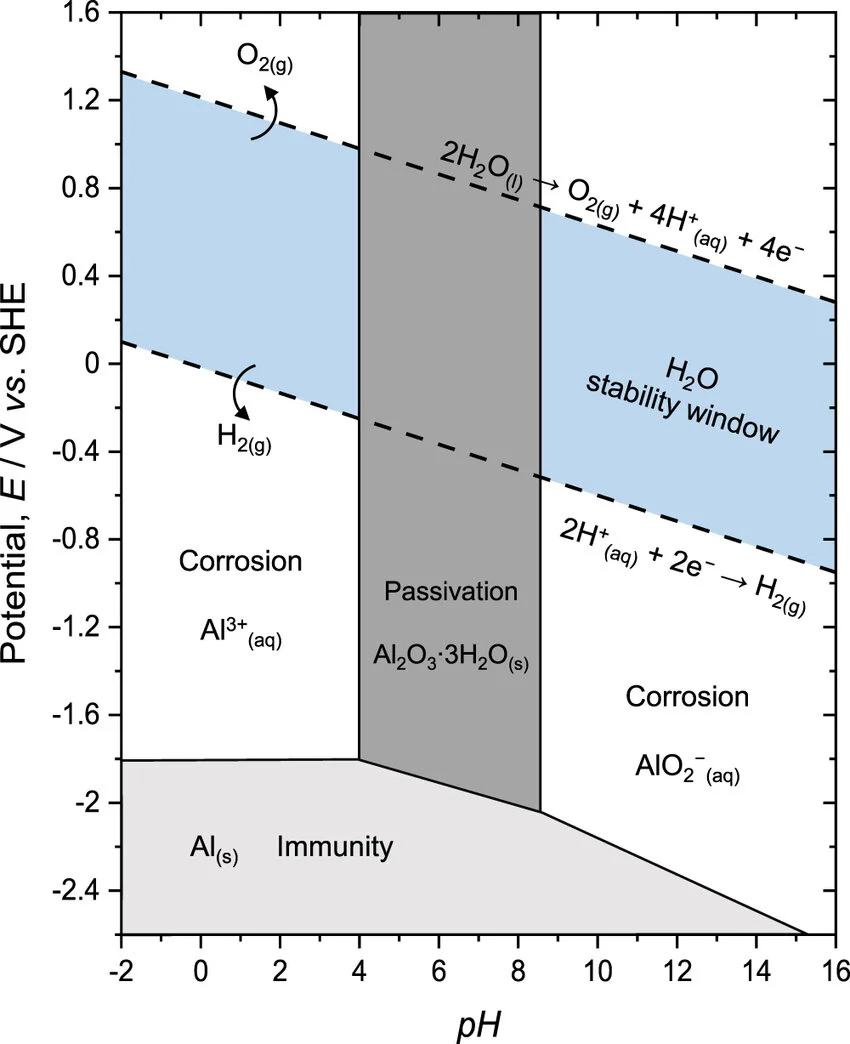
\includegraphics[width=0.35\textwidth]{figs/pourbaix.png} 
    \caption{Pourbaix diagram of aluminium.}
    \label{fig:pourbaix}
\end{figure}


\section{Breakdown of Passivity by Chloride} %% PENDING REVIEW (DONE)
\label{sec:chloride}

Although the native alumina film confers effective passivation across a broad pH range, it is particularly vulnerable to localised breakdown in the presence of chloride ions \cite{Vargel2020, Sastri2007}. Due to their small ionic radius and low hydration energy, chloride ions readily shed their hydration shell and adsorb directly onto the oxide surface, competing with hydroxyl ions for adsorption sites at surface defects, grain boundaries, and IMP/matrix interfaces \cite{Vargel2020, Zhang2018, McCafferty2010}:

\begin{equation}
    \mathrm{Al(OH)_{ads}} + \mathrm{Cl^{-}} \rightarrow \mathrm{AlCl_{ads}} + 
    \mathrm{OH^{-}}
    \label{eq:cl_adsorption}
\end{equation}

Once a critical local chloride concentration is reached, the passive film ruptures and the exposed aluminium undergoes accelerated anodic dissolution, generating soluble chloride complexes that hydrolyse to produce a locally acidic environment, further accelerating dissolution and inhibiting repassivation \cite{Vargel2020, Ghali2010}. This transition is characterised by the pitting potential ($E_{\text{pit}}$), above which localised attack proceeds spontaneously and the autocatalytic pit growth mechanism described in Section~\ref{sec:pitting} is activated \cite{Revie2008, Ghali2010}. This underscores the need for active corrosion protection systems capable of suppressing film breakdown and restoring passivity at localised defects \cite{MartinezViademonte2020, BoualiReview2020}.


\section{Kinetics of Corrosion}
\label{sec:kinetics}

The kinetics of corrosion are fundamentally governed by the rate of charge transfer at the interface between a metal and its surrounding aqueous environment \cite{Vargel2020}. During corrosion, metal atoms are oxidised at anodic sites, releasing electrons into the metal lattice, while electroactive species in solution simultaneously capture these electrons at cathodic sites \cite{Vargel2020}. These two partial reactions are spatially and electrically coupled, and their relative rates determine the overall corrosion rate.

This charge exchange is confined to a highly structured interfacial region, approximately 10~nm in thickness, known as the electrical double layer (Figure~\ref{fig:double_layer}) \cite{Vargel2020}. Upon immersion of a metal in an electrolyte, the perturbation of the local molecular and ionic arrangement gives rise to a charge separation at the interface, which is sustained to maintain overall electroneutrality \cite{Vargel2020, Sastri2007}. The resulting double layer is structurally described by a combination of the Helmholtz, Stern, and Gouy--Chapman models, which together delineate three regions of decreasing order moving away from the surface \cite{Vargel2020, Sastri2007}. The innermost compact Stern layer contains oriented water molecules and specifically adsorbed species; of particular relevance is the adsorption of chloride ions, which --- owing to their small ionic radius and low hydration energy --- readily shed their hydration shell to adsorb directly onto the metal surface, locally disrupting the passive oxide film and rendering them the primary initiator of pitting corrosion \cite{Vargel2020, Sastri2007}. Beyond this lies the outer Helmholtz plane, marking the closest approach of solvated ionic species that retain their hydration shell \cite{Vargel2020, Sastri2007}. Further out, the diffuse Gouy--Chapman layer extends into the bulk electrolyte, consisting of a loosely organised ionic distribution whose thickness decreases with increasing electrolyte concentration \cite{Vargel2020, Sastri2007}.

The architecture of the double layer directly controls corrosion kinetics by imposing physical and electrostatic barriers to ionic transport and charge transfer \cite{Sastri2007}.

\begin{figure}[htbp]
    \centering
    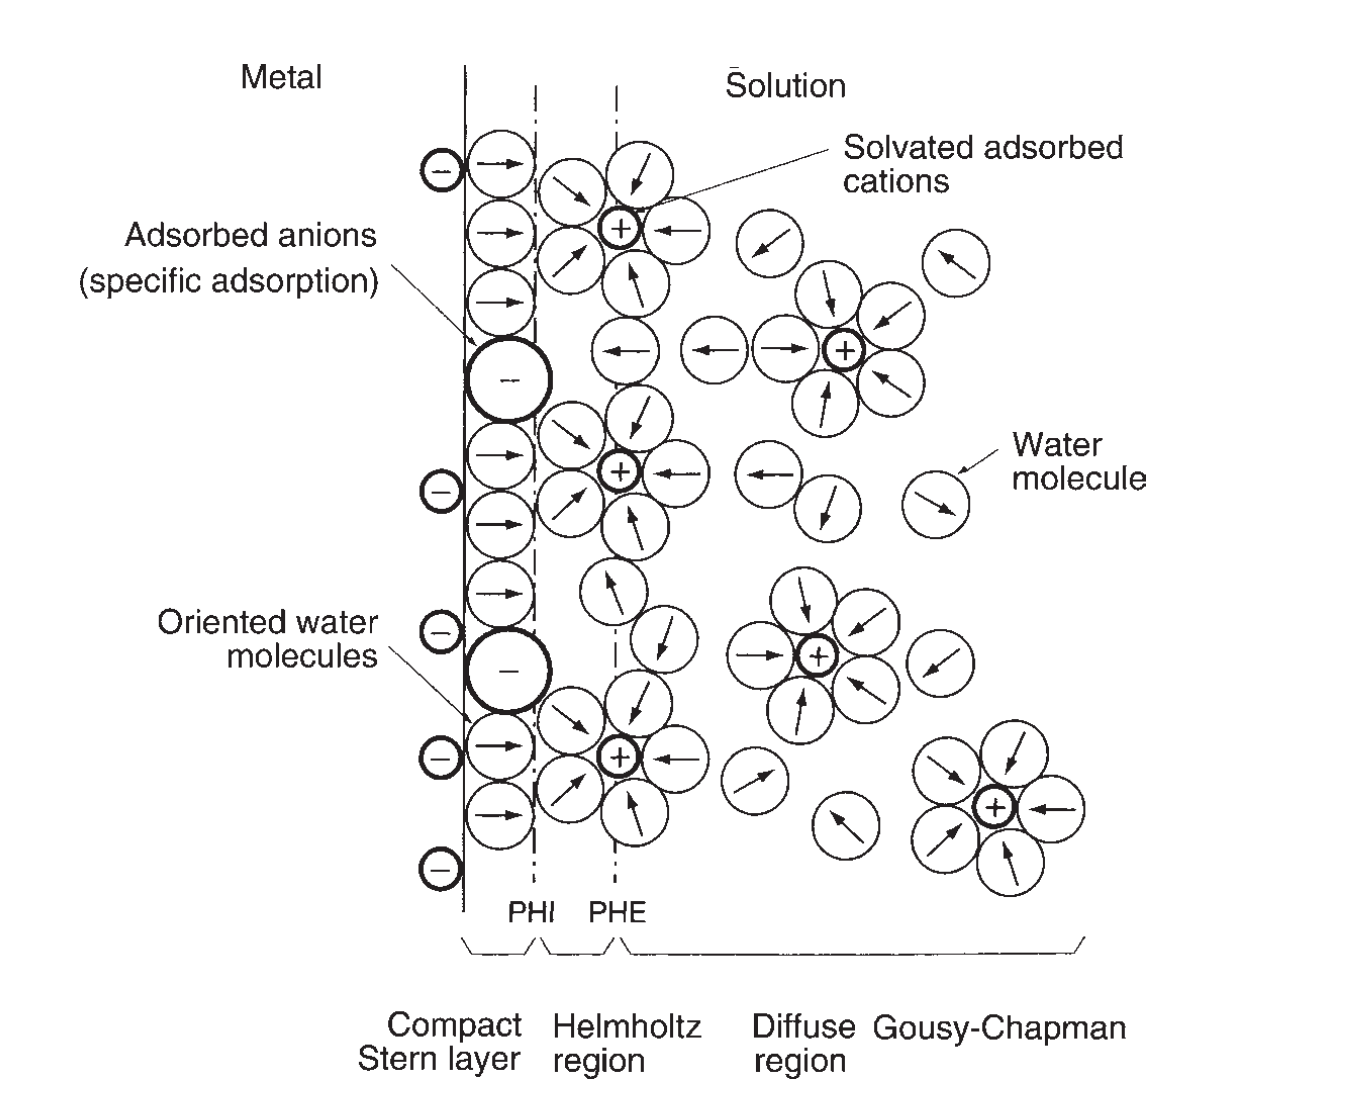
\includegraphics[width=0.4\textwidth]{figs/double_layer.png} 
    \caption{Metal--solution interface: double layer.}
    \label{fig:double_layer}
\end{figure}

\section{Pitting Corrosion of Aluminium Alloys} %%PENDING REVIEW (DONE)
\label{sec:pitting}

While the passive oxide film that forms spontaneously on aluminium provides effective protection across a broad range of conditions, it is susceptible to localised breakdown in the presence of aggressive anions, most notably chloride \cite{Vargel2020, Revie2008}. This breakdown initiates pitting corrosion, a highly localised form of attack in which small, discrete cavities propagate into the metal while the surrounding surface remains nominally passive \cite{Vargel2020, Sastri2007}.

Pit initiation is strongly associated with the presence of IMPs at the alloy surface. As described in Section~\ref{sec:kinetics}, chloride ions preferentially adsorb at defect sites or at boundaries between IMPs and the aluminium matrix, where they locally displace oxygen and hydroxide ions from the passive film \cite{Vargel2020,Zhang2018,Ghali2010, McCafferty2010} (Figure~\ref{fig:pitting}). Once a critical chloride concentration is reached at these sites, the passive film ruptures and active dissolution of the underlying metal commences \cite{Vargel2020,Revie2008}. This breakdown is characterised by a transition from passive to active behaviour at a potential known as the pitting potential ($E_{\text{pit}}$), below which the passive film is stable \cite{Revie2008, Ghali2010}.

\begin{figure}[htbp]
    \centering
    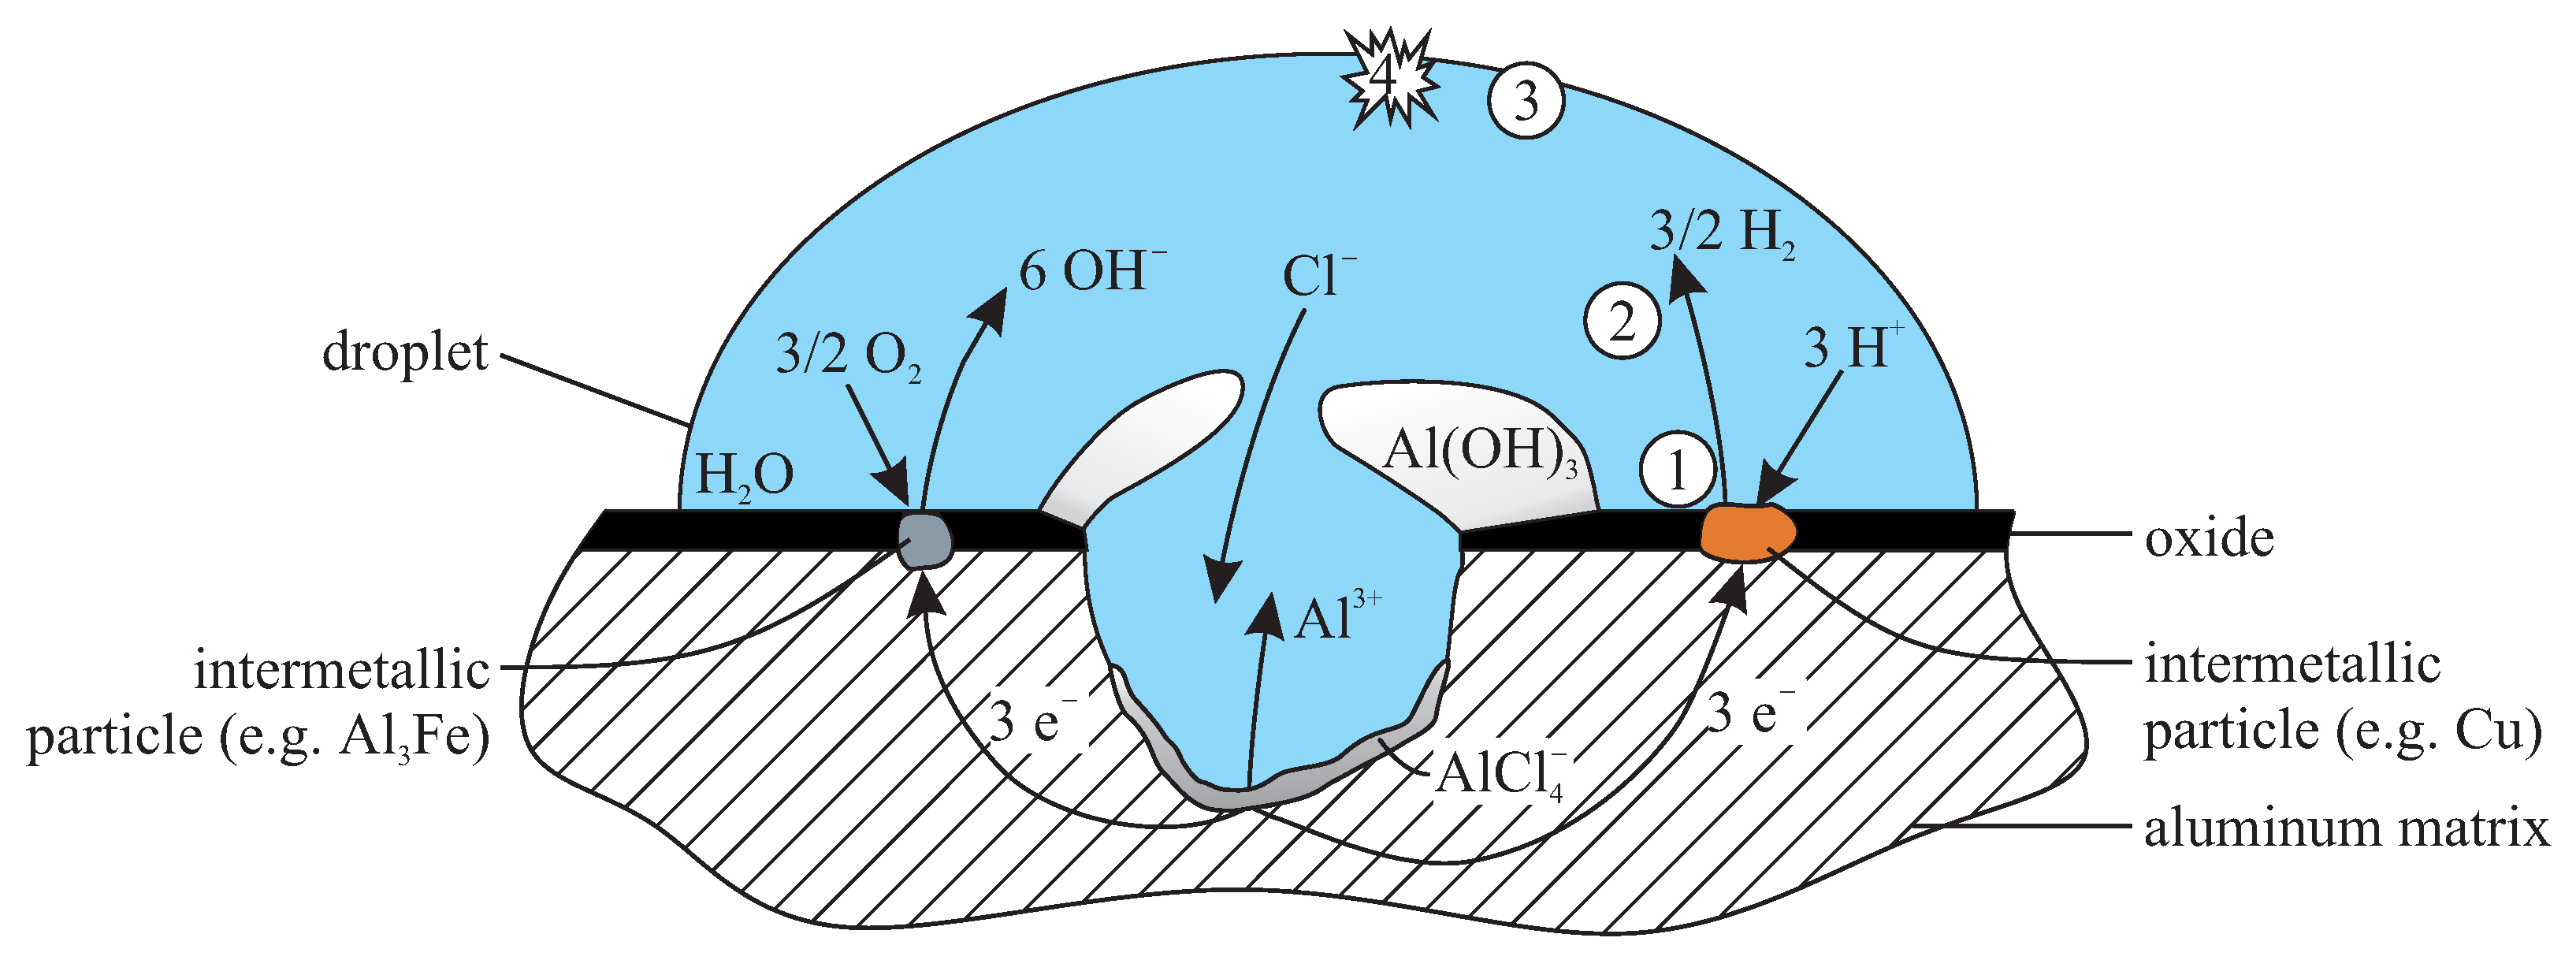
\includegraphics[width=0.5\textwidth]{figs/pitting.png} 
    \caption{Pitting mechanism of cathodic intermetallics in aluminium.}
    \label{fig:pitting}
\end{figure}

Following initiation, pit growth is sustained by an autocatalytic mechanism \cite{Sastri2007,Ghali2010}. Metal dissolution within the pit generates a local excess of cations, which attracts additional chloride ions to maintain charge balance \cite{Vargel2020,Ghali2010,Sastri2007}. The resulting accumulation of metal chloride salts undergoes hydrolysis, acidifying the pit interior and further accelerating dissolution \cite{Revie2008, Sastri2007,Ghali2010,Vargel2020}. The surrounding cathodic regions support the oxygen reduction reaction, maintaining the electrochemical driving force for continued pit growth \cite{Revie2008, Sastri2007,Ghali2010,Vargel2020}. Prior to reaching a stable propagating state, pits may repeatedly initiate and repassivate, a phenomenon known as metastable pitting, which is observable electrochemically as transient current fluctuations at potentials below $E_{\text{pit}}$ \cite{Sastri2007, Ghali2010}.

From a protective coating perspective, the critical objective is therefore not only to provide a barrier against electrolyte ingress, but also to supply active inhibition that can suppress these autocatalytic processes should the barrier be locally breached \cite{MartinezViademonte2020, BoualiReview2020}.

\section{Conventional Corrosion Protection Methods}
\label{sec:conventional}

Conventional corrosion protection systems for aluminium alloys, particularly in aerospace applications, typically consist of a multilayer structure comprising an anodic oxide or conversion coating, followed by a corrosion-inhibited primer and an organic topcoat \cite{MartinezViademonte2020}. These systems are designed to provide both passive barrier protection and active corrosion inhibition, and their general architecture is illustrated in Figure~\ref{fig:multilayer}.

\begin{figure}[htbp]
    \centering
    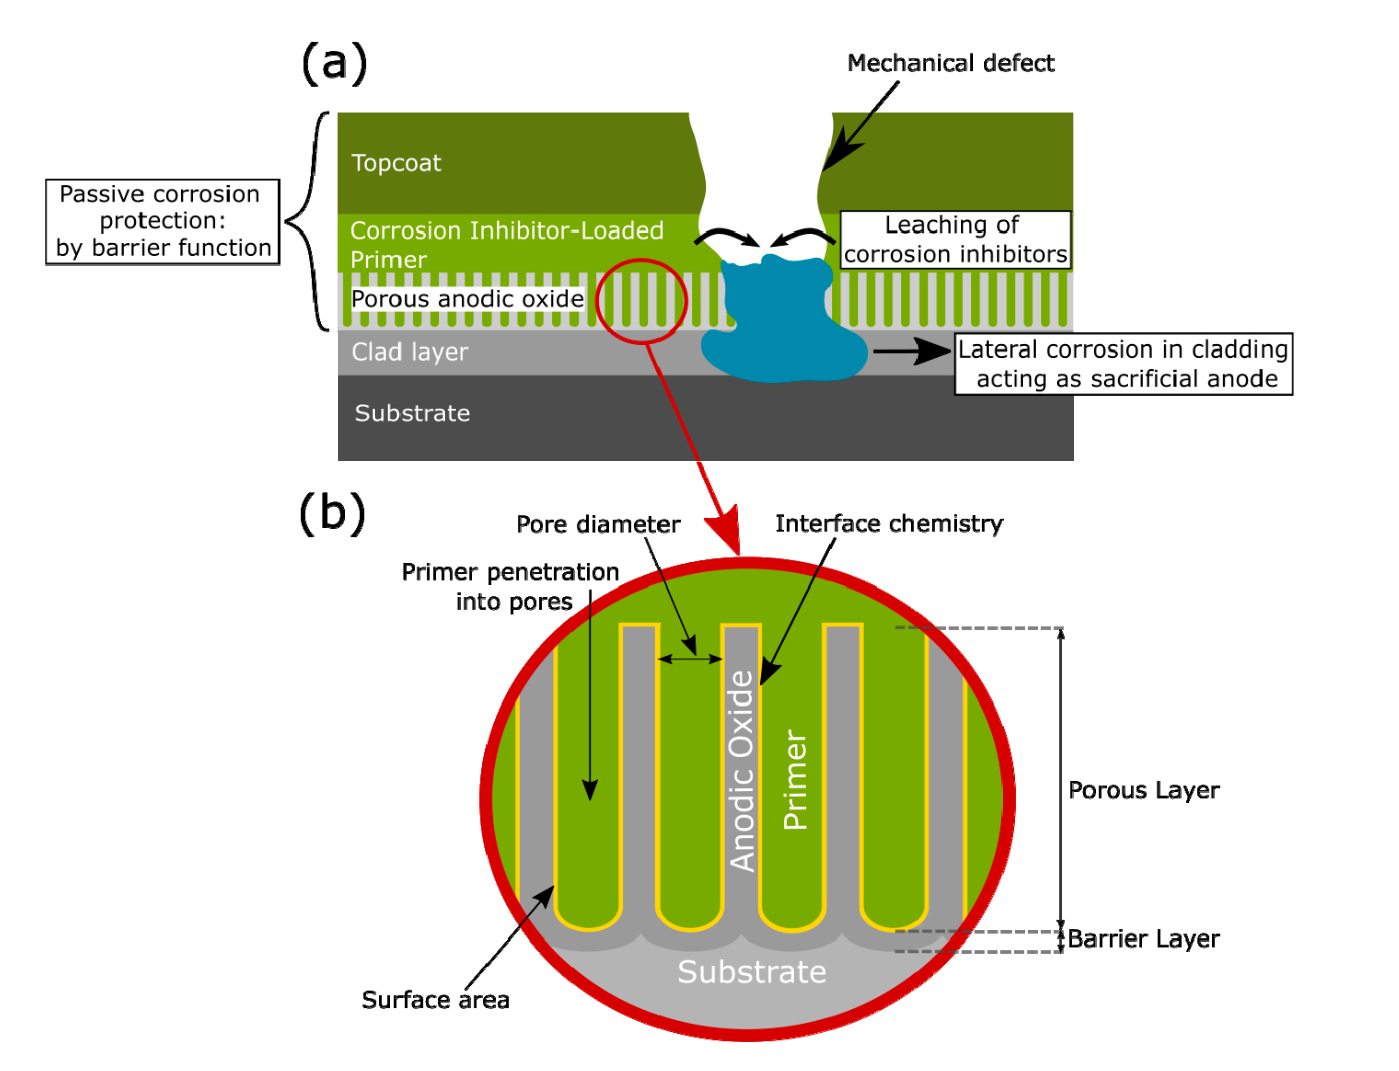
\includegraphics[width=0.5\textwidth]{figs/multilayer.png} 
    \caption{Typical multilayer coating system for corrosion protection of 
    aluminium alloys.}
    \label{fig:multilayer}
\end{figure}

Passive protection is provided by the coating layers themselves, which act as a physical barrier against electrolyte ingress, while active protection is achieved through corrosion inhibitors incorporated into the primer that become mobilised when coating defects allow electrolyte contact with the substrate \cite{MartinezViademonte2020}. Anodising is an electrochemical process in which the aluminium surface is oxidised under an applied anodic potential in an acidic electrolyte, forming a thick, porous aluminium oxide layer that provides significantly enhanced corrosion and wear resistance relative to the native passive film \cite{MartinezViademonte2020}. The resulting oxide consists of a thin, compact barrier layer at the metal/oxide interface and a thicker porous outer layer, whose characteristics are governed by the electrolyte composition, applied voltage, and treatment duration \cite{MartinezViademonte2020}. Although anodised aluminium alloys generally exhibit superior corrosion and wear resistance, conversion coatings (CCs) are often preferred in industrial practice due to their lower cost, simpler processing, and greater application flexibility \cite{Becker2019}.

Historically, hexavalent chromium has played a central role in these protection systems, both as the basis of chromate conversion coatings (CCCs) and as a leachable inhibitor within primers, owing to its well-documented self-healing capability \cite{Beneke2016, BoualiReview2020}. However, Cr(VI) compounds are classified as highly toxic and carcinogenic, and their use is now subject to severe regulatory restrictions, creating an urgent need for environmentally benign alternatives \cite{MartinezViademonte2020, BoualiReview2020}.

Among the proposed replacements, trivalent chromium process (TCP) coatings have gained industrial acceptance but exhibit reduced effectiveness with non-chromium primers and raise concerns over trace Cr(VI) formation during processing \cite{Becker2019, Qi2015, BoualiReview2020}. Rare earth conversion coatings (RECCs), particularly cerium-based systems, have also been investigated, offering lower toxicity and comparable performance to CCCs \cite{Becker2019, Hughes2009}; however, their lack of robust self-healing and sensitivity to substrate chemistry have limited industrial adoption \cite{Becker2019}. 

%%ADD ANODISING HERE BUT INCORPORATE WITH THE REST OF THE TEXT

\section{Layered Double Hydroxides as a Chromate-Free Alternative}
\label{sec:LDH}

More recently, layered double hydroxides (LDHs) have emerged as a promising chromate-free alternative for corrosion protection. LDHs belong to a class of lamellar materials with brucite-like structures (Figure~\ref{fig:ldh_strucutre}), consisting of positively charged metal hydroxide host layers with exchangeable anions located in the interlayer galleries to maintain charge balance \cite{Bouali2020, Zhou2017, He2020, Iuzviuk2020, Cao2022}. Their general chemical formula is:

\begin{equation}
    [\mathrm{M}^{2+}_{1-x}\mathrm{M}^{3+}_{x}(\mathrm{OH})_{2}]^{x+}
    (\mathrm{A}^{n-})_{x/n} \cdot m\mathrm{H}_{2}\mathrm{O}
    \label{eq:LDH}
\end{equation}

where $\mathrm{M}^{2+}$ and $\mathrm{M}^{3+}$ represent the divalent and trivalent metal cations, $\mathrm{A}^{n-}$ the $n$-valent interlayer anions, $x$ the molar ratio $\mathrm{M}^{3+}/(\mathrm{M}^{2+} + \mathrm{M}^{3+})$ (typically 0.2--0.33), and $m$ the number of interlayer water molecules \cite{He2020, Cao2022}. The cation composition is highly tuneable, provided the ionic radii are compatible with octahedral coordination in the hydroxide layer \cite{He2020}. The relatively weak electrostatic and hydrogen bonding interactions between the layers and interlayer anions confer LDHs with their most technologically relevant property: facile anion exchange, whereby inhibiting anions pre-loaded into the interlayer galleries are released in exchange for aggressive species such as chloride upon electrolyte ingress \cite{Bouali2020, BoualiReview2020} (Figure~\ref{fig:ldh_mechanism}). This ion-exchange mechanism provides an active, self-healing corrosion inhibition capability analogous to chromate-based systems but without the associated toxicity, and has been demonstrated on aluminium, zinc, and magnesium alloys, as well as anodised surfaces and galvanised steels \cite{Iuzviuk2020, Buchheit2003}.

\begin{figure}[htbp]
    \centering
    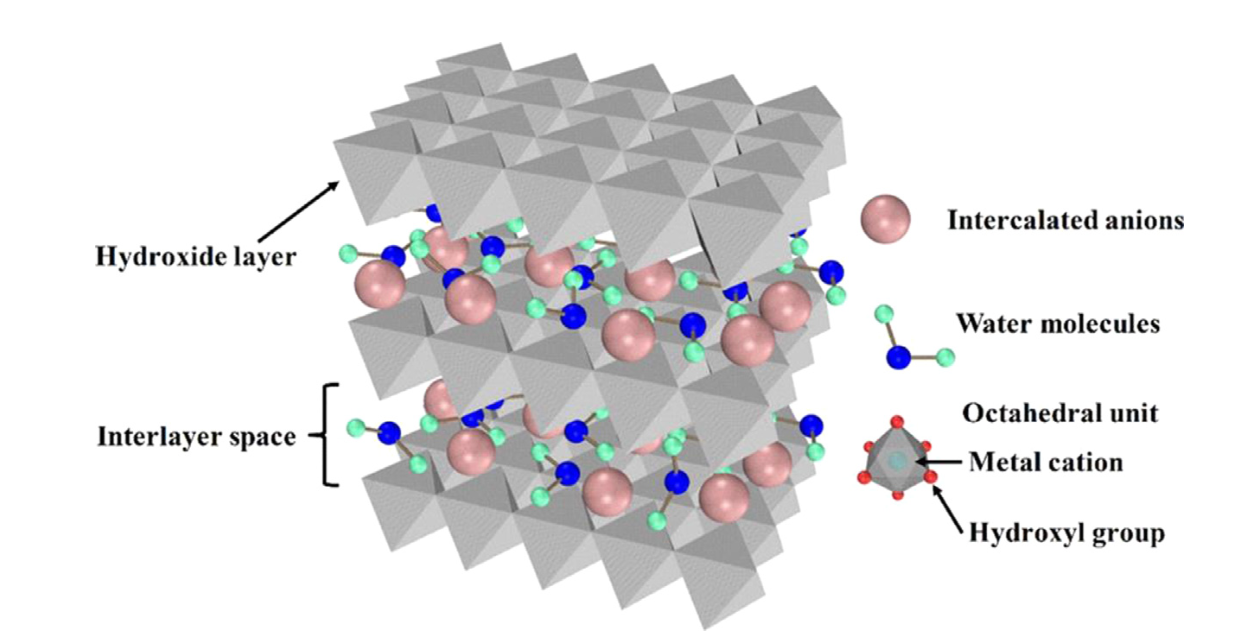
\includegraphics[width=0.5\textwidth]{figs/ldh_structure.png} 
    \caption{Schematic structure of LDH.}
    \label{fig:ldh_strucutre}
\end{figure}

\begin{figure}[htbp]
    \centering
    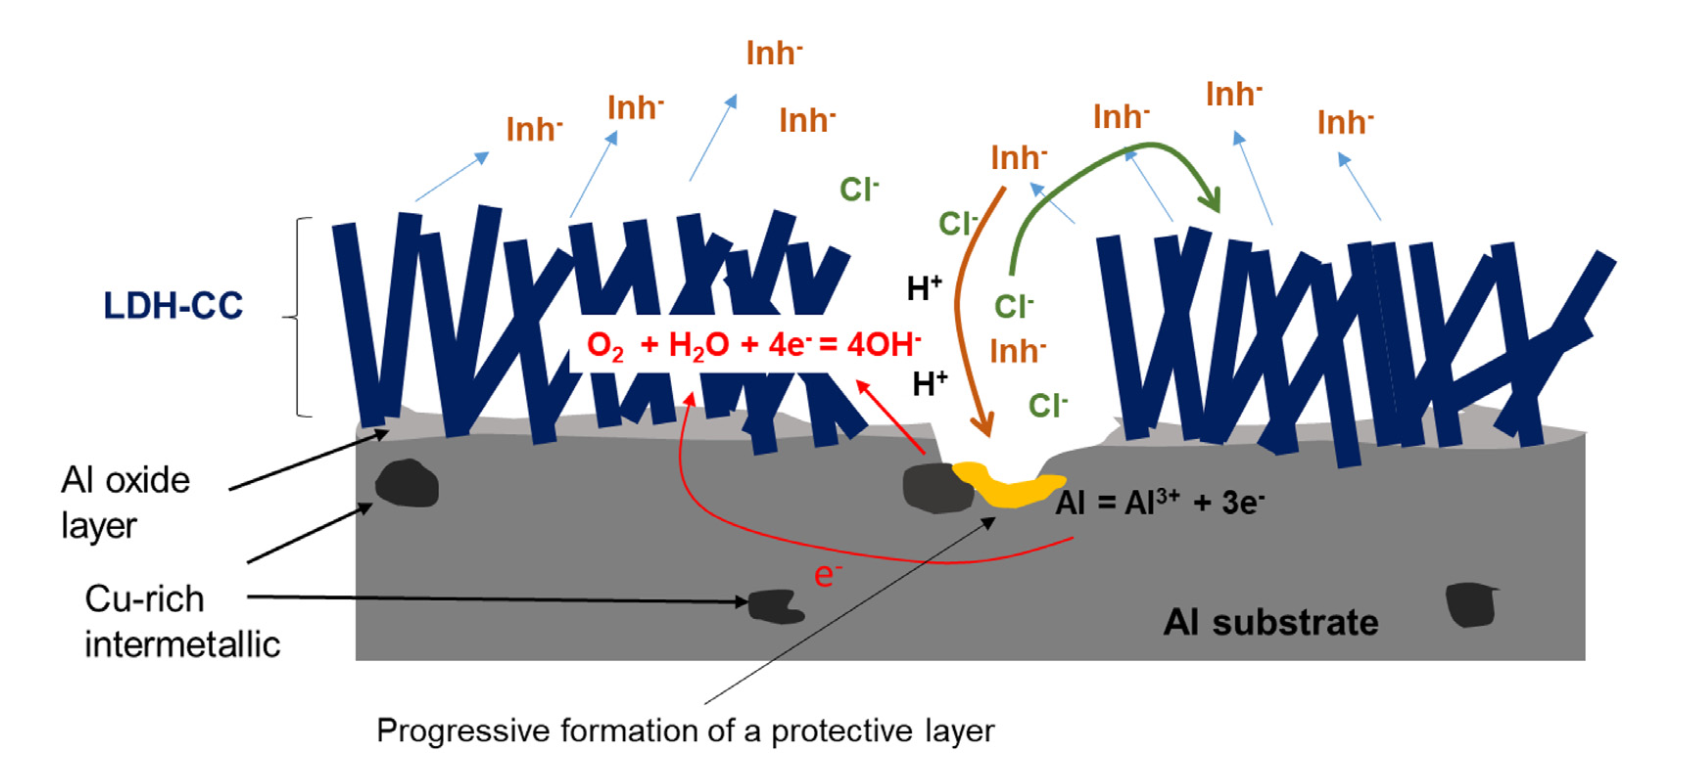
\includegraphics[width=0.5\textwidth]{figs/ldh_mechanism.png} 
    \caption{Scheme describing the corrosion protection mechanism of LDH conversion coating on an Al substrate.}
    \label{fig:ldh_mechanism}
\end{figure}

\subsection{Advantages of LDH}
\label{subsec:LDH_advantages}

The anion exchange capability of LDHs can be exploited in two complementary ways for corrosion protection \cite{Iuzviuk2020, He2020, Cao2022, Zhou2017, Bouali2020}:

\begin{enumerate}
    \item \textbf{Controlled release of corrosion inhibitors:} LDHs act as hosts for anionic inhibitors pre-loaded into their interlayer galleries, releasing them on demand in response to local pH changes or the ingress of aggressive anions (e.g.\ $\mathrm{Cl}^{-}$, $\mathrm{SO}_4^{2-}$), achieving self-healing performance comparable to Cr(VI)-based systems \cite{Bouali2020, BoualiReview2020};

    \item \textbf{Trapping of aggressive species:} LDHs simultaneously capture harmful anions --- most notably chloride --- within their interlayer galleries, reducing the local concentration of corrosive species at the metal surface \cite{Iuzviuk2020, He2020}.
\end{enumerate}

Beyond anion exchange, LDHs are capable of local dissolution and recrystallisation at coating defects, restoring barrier integrity and reinforcing self-healing behaviour \cite{Cao2022}. Synergistic effects between multiple protection mechanisms can further enhance overall performance beyond the sum of individual contributions \cite{Cao2022}.

\subsection{Synthesis of LDH}
\label{subsec:LDH_synthesis}

LDHs can be fabricated either ex situ as powders or in situ as films grown directly on metal substrates. Ex situ LDH powders are most commonly synthesised by co-precipitation, which can be carried out under variable or constant pH conditions \cite{BoualiReview2020}. Once synthesised, LDH powders can be dispersed within single-layer coating systems, such as sol--gel hybrid coatings \cite{Yasakau2014, Alvarez2010}, or distributed across multilayer coating architectures, which is a common approach in industrial applications such as the automotive sector \cite{BoualiReview2020}.

Despite this versatility, in situ LDH growth is generally considered more advantageous for corrosion protection, as it promotes the formation of chemical bonds between the LDH film and the substrate, resulting in stronger interfacial adhesion \cite{BoualiReview2020, Cao2022, Guo2009}. Furthermore, in situ film formation is a single-step process that is largely independent of substrate geometry, making it well suited for large-area and complex-geometry applications \cite{Guo2009, BoualiReview2020}.

The most widely adopted in situ method is hydrothermal treatment, also referred to as in situ co-precipitation by some authors \cite{BoualiReview2020}, which can be regarded as an extension of the ex situ co-precipitation approach. In this work, the approach described by \citet{BoualiReview2020} is adopted, in which the substrate itself serves as one of the metal precursors. For aluminium substrates, LDH films are grown by immersing the substrate in a solution containing divalent or monovalent metal cations (such as $\mathrm{Zn}^{2+}$, $\mathrm{Mg}^{2+}$, or $\mathrm{Li}^{+}$) under controlled pH, temperature, and concentration conditions, while $\mathrm{Al}^{3+}$ ions are supplied through partial dissolution of the substrate. This approach produces strong interfacial bonding between the LDH film and the substrate \cite{Cao2022, Guo2009}, and has been employed in numerous corrosion protection studies \cite{Iuzviuk2020, Tedim2014, Tedim2011}.

Beyond hydrothermal treatment, alternative in situ fabrication routes have been explored, including electrodeposition, which offers shorter processing times but generally yields weaker adhesion \cite{He2020, Cao2022}, and steam coating, which combines good bonding strength with an environmentally benign process \cite{Pan2023, Cao2022}.

\subsection{Rationale for ZnAl--LDH on Aluminium Substrates} %% PENDING REVIEW (DONE)
\label{subsec:ZnAl}

Among the many possible LDH compositions, ZnAl--LDH has emerged as one of the most studied systems for in situ corrosion protection of aluminium alloys. This preference is grounded in both chemical compatibility and processing considerations. As describedin Section~\ref{subsec:LDH_synthesis}, in situ hydrothermal synthesis on aluminium substrates relies on the partial dissolution of the substrate to supply the trivalent$\mathrm{Al}^{3+}$ cation, while the divalent cation is provided externally through the synthesis solution \cite{BoualiReview2020,Cao2022}. Among the candidate divalent cations, $\mathrm{Zn}^{2+}$ is particularly well suited: its ionic radius is compatible with octahedral coordination in the brucite-like layer, and zinc-based LDH systems have consistently demonstrated effective anion exchange kinetics and strong inhibitor release behaviour in chloride-containing environments \cite{Bouali2020, Tedim2011, BoualiReview2020,Cao2022}. The combination of established synthesis protocols, well-documented inhibitor intercalation behaviour, and demonstrated performance on aluminium alloys therefore makes ZnAl--LDH the most appropriate system for the present study.

\subsection{Corrosion Inhibitors}
\label{subsec:inhibitors}

LDHs are typically synthesised with nitrate ions as the initial interlayer anions, owing to their weak affinity for the LDH structure and consequently high exchangeability. Carbonate anions, by contrast, exhibit a significantly stronger affinity and therefore resist subsequent exchange, making them unsuitable as precursor anions \cite{Cao2022}. Once synthesised, the LDH undergoes an anion-exchange step to intercalate the desired corrosion inhibiting species. Unlike inorganic inhibitors such as vanadate, thiol-containing organic inhibitors such as MBT require deprotonation into their anionic form prior to intercalation, as their neutral forms exhibit insufficient aqueous solubility and lack the negative charge required for electrostatic uptake into the positively charged LDH interlayer galleries. This is achieved by adjusting the solution pH with \ce{NaOH}, which converts the neutral molecule into its soluble anionic form.

Vanadates are among the most extensively studied inhibitor systems, with active corrosion protection of AA2024 demonstrated by \citet{Tedim2011} and \citet{Yasakau2014}. \citet{Zhang2015} further showed that vanadate-intercalated ZnAl--LDH provides superior corrosion resistance relative to nitrate-intercalated LDH on the same alloy, while \citet{Zhou2017} reported analogous protective behaviour for AZ91 magnesium alloy. Other inhibitors, including MBT and molybdate, have also been investigated \cite{Cao2022, Tedim2010, Zhang2015}; however, for AA2024 these were found to offer inferior corrosion protection relative to vanadates \cite{Zhang2015, Tedim2010}. The relative performance of inhibitors is strongly dependent on both the LDH composition and the substrate chemistry: \citet{Matsui2025} reported that molybdate-intercalated Mg--Al LDH provided superior corrosion resistance compared to vanadate-based systems on ADC-12, an Al--Si--Cu die-cast alloy, underscoring the importance of tailoring inhibitor selection to the specific alloy system under investigation.

\section{Influence of IMPs on LDH growth}

AC46000 contains a diverse range of intermetallic particles (IMPs), including copper-rich phases such as \ce{Al2Cu} and \ce{Al7Cu2Fe}, iron-rich phases such as \ce{Al5FeSi} and \ce{Al15(Fe,Mn)3Si2}, and eutectic silicon particles. To assess the influence of these IMPs on LDH growth and corrosion behavior, it is important to consider their electrochemical potential relative to the aluminium matrix \cite{Gudic2024,Kasinska2020}.

The copper-rich phases are strongly cathodic relative to the Al matrix, with \ce{Al2Cu} exhibiting a potential difference of approximately +400 mV \cite{Gudic2024}. This drives intense localized micro-galvanic coupling, promoting rapid oxygen reduction and a sharp rise in local pH. In the context of LDH growth, these conditions trigger the preferential and rapid precipitation of thick, "flower-like" LDH islands directly over the cathodic sites \cite{Cao2026} (Figure~\ref{fig:ldh_nucleation}). This localized growth is sustained by the anodic dissolution of the surrounding aluminium matrix, commonly referred to as trenching \cite{Bouali2022}. The trenching process generates voids at the periphery of the intermetallic particles where LDH flakes fail to nucleate \cite{Bouali2022}. These uncoated gaps compromise the corrosion resistance of the substrate, as chloride ions and other aggressive species can readily penetrate the exposed defects and initiate pitting corrosion \cite{Bouali2022}. The resulting inhomogeneous LDH film also reduces the adhesion of subsequently applied polymer coatings or paints \cite{Bouali2022}, and in severe cases extensive trenching can render the intermetallic particles prone to detachment, further undermining the integrity of overlying layers \cite{Bouali2022}.

\begin{figure}[htbp]
    \centering
    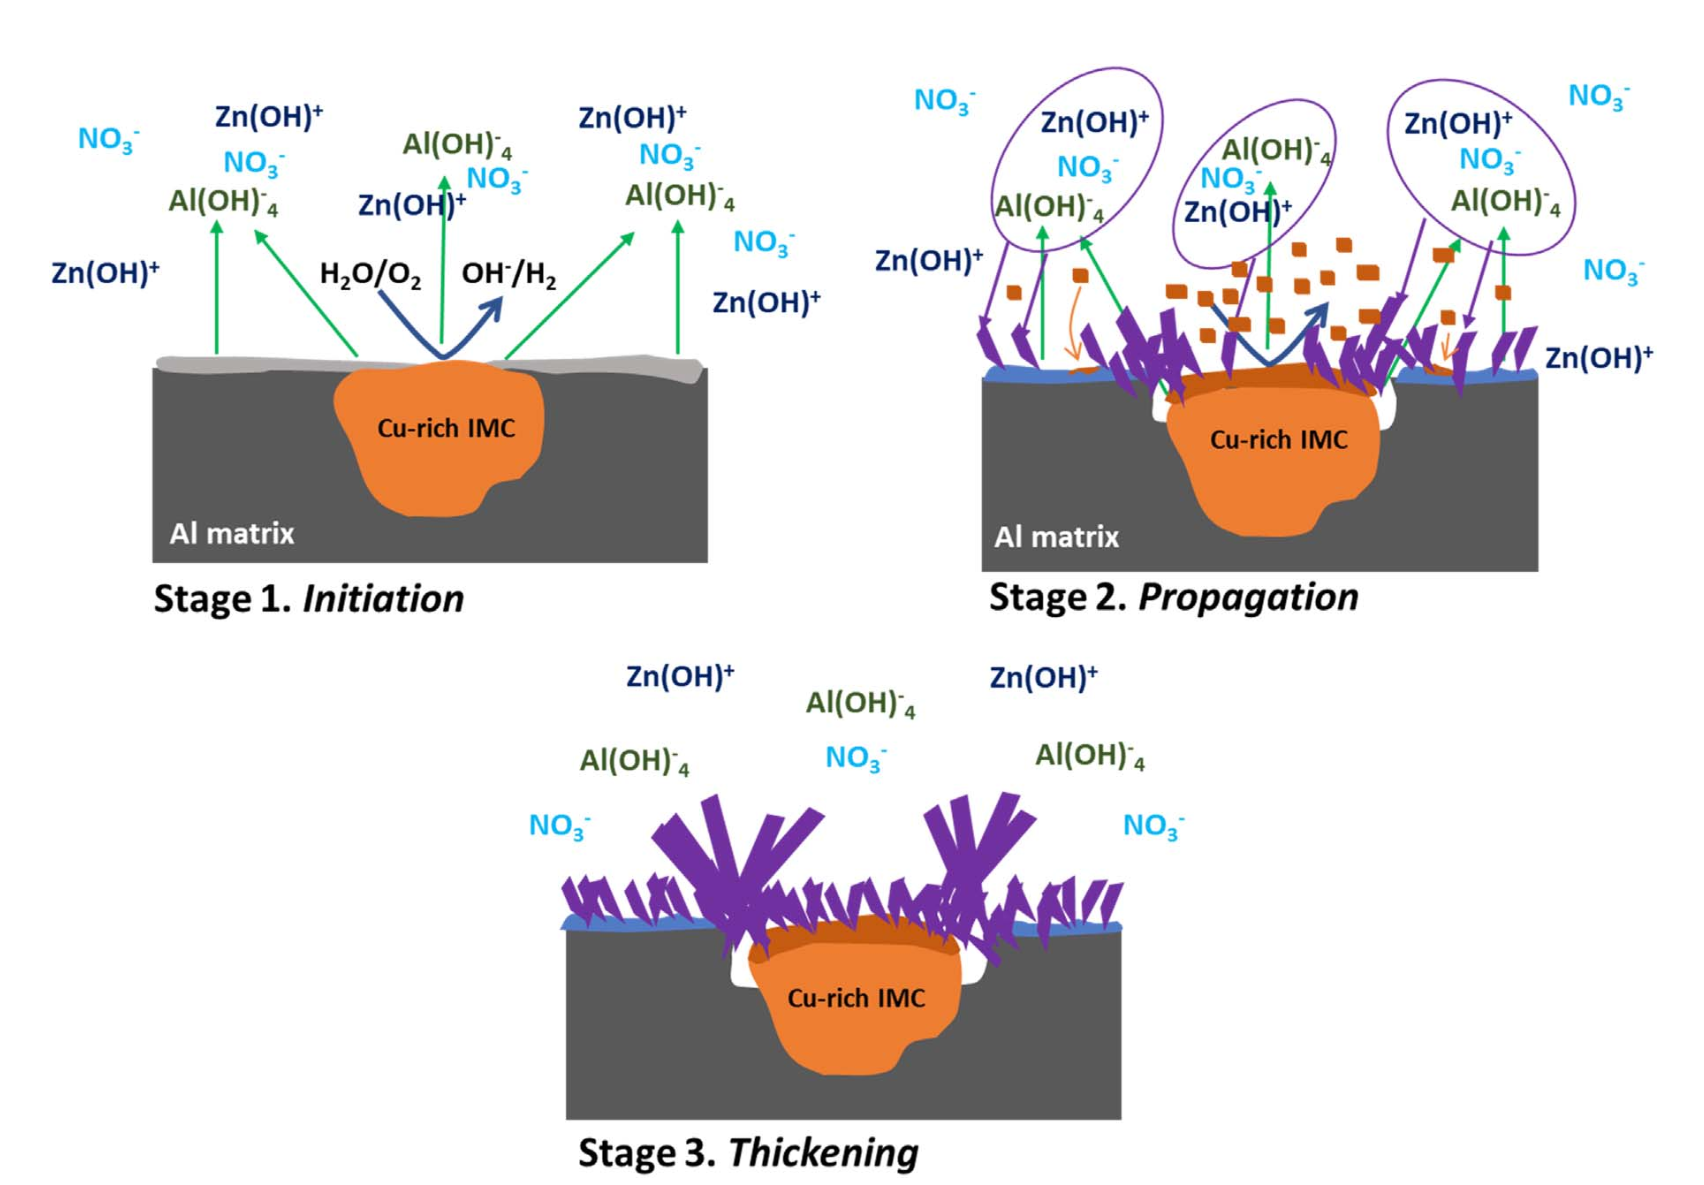
\includegraphics[width=0.65\textwidth]{figs/ldh_nucleation.png} 
    \caption{Generalized mechanism of LDH growth on a Cu-rich IMC in aluminium alloy.}
    \label{fig:ldh_nucleation}
\end{figure}

The iron-rich phases are also strongly cathodic, approximately +300 mV above the aluminium matrix \cite{Gudic2024}, and the galvanic coupling they generate similarly leads to inhomogeneous LDH growth and increased susceptibility to corrosion.

Although eutectic silicon particles are likewise cathodic, with a potential difference of approximately +250 mV relative to the Al matrix, they are electrochemically inert and do not act as nucleation sites for LDH. Since they provide no source of the metal cations (\ce{Al^2+/Al^3+}, \ce{Mg^2+}) required for LDH formation, as was explained in section \ref{subsec:LDH_synthesis}, no coating growth is triggered at these sites \cite{Gudic2024,DelOlmo2025}.

\subsection{Pre-Treatment}

Given the detrimental influence of these IMPs on LDH growth homogeneity and overall coating quality, their removal from the alloy surface prior to conversion coating is essential. To this end, various pre-treatment strategies have been developed, but the most widely adopted approach consists of a multistep procedure comprising degreasing, alkaline etching, and acid pickling, applied sequentially \cite{MartinezViademonte2020}.

Degreasing constitutes the first pre-treatment step, with the primary objective of removing surface contamination, most notably oils and lubricants introduced during the manufacturing process. This step is critical to ensure full surface wettability, thereby guaranteeing that subsequent processing stages act uniformly across the substrate \cite{MartinezViademonte2020}. 

The second step, alkaline etching, is aimed at dissolving the native oxide layer that forms spontaneously on aluminium surfaces, as well as removing surface-exposed intermetallic particles. The cathodic IMPs act as highly active sites for oxygen reduction, generating a localised rise in pH at their immediate vicinity. This accelerates the anodic dissolution of the surrounding aluminium matrix, progressively undermining the mechanical support of the particles \cite{Nelson2001}. As the matrix recedes, scallop-shaped voids form at the particle periphery, eventually causing the IMPs to detach from the surface, a process known as selective dealloying \cite{Nelson2001,Jin2020}. Since many of the constituent alloying elements released during this process are insoluble in alkaline media, they accumulate on the surface as a loosely adherent residue known as smut, the removal of which necessitates a subsequent acid pickling step \cite{MartinezViademonte2020,Nelson2001,Jin2020}.

Nitric acid (\ce{HNO3}) is widely used for desmutting because it naturally passivates the aluminum matrix while acting as a powerful oxidant \cite{Jin2020}. It successfully targets and dissolves the dealloyed metallic smut, including copper, iron, and manganese residues. Despite this, Nitric acid alone is ineffective against silicon eutectic phases \cite{ASM1994}. To remove these, fluorides (such as hydrofluoric acid or ammonium bifluoride) must be added to the pickling bath \cite{Askin1995,Lee2008}. The fluoride ions dissolve the silica and complex the remaining silicon remnants so they can be washed away \cite{Askin1995,Lee2008}.

\section{Equivalent Circuit Models for EIS}
\subsection{Randles Equivalent Circuit (REC)}

Determining an appropriate equivalent circuit model (ECM) for electrochemical impedance spectroscopy (EIS) spectra is among the most critical steps in impedance analysis, as it enables the deconvolution of overlapping electrochemical processes and their quantification through physically meaningful parameters. One of the most widely used models is the Randles equivalent circuit, which consists of a solution resistance ($R_{\text{s}}$) in series with a parallel combination of a charge-transfer resistance ($R_{\text{ct}}$) and a double-layer capacitance ($C_{\text{dl}}$), as represented in Figure~\ref{fig:randles} \cite{Das2025, Lasia2014}.

\begin{figure}[htbp]
    \centering
    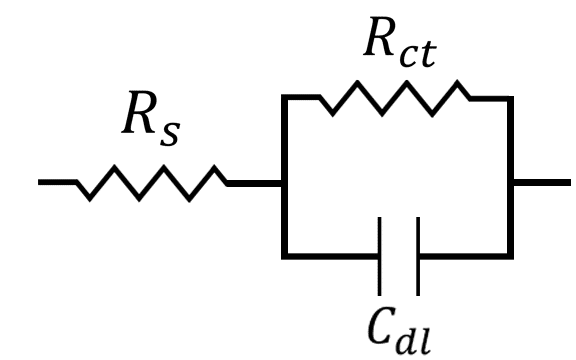
\includegraphics[width=0.25\textwidth]{figs/randles.png} 
    \caption{Randles equivalent circuit.}
    \label{fig:randles}
\end{figure}


\subsubsection{Solution Resistance}
$R_{\text{s}}$, also referred to as the ohmic or solution resistance, quantifies the resistive potential drop occurring between the working electrode and the reference electrode \cite{MetrohmEIS3, Lasia2014}. Its magnitude is governed by the specific conductivity of the bulk electrolyte and the cell geometry \cite{MetrohmEIS3}. In a Nyquist representation, $R_{\text{s}}$ is readily identified as the high-frequency intercept of the impedance data with the real axis, corresponding to the condition under which the reactive elements of the circuit are effectively short-circuited and the purely resistive contribution dominates the response.

\subsubsection{Charge-Transfer Resistance}
$R_{\text{ct}}$ is the real component of the Faradaic impedance governing the transfer of electrons across the electrode/electrolyte interface to or from electroactive species in solution \cite{Lasia2014}. As a strictly kinetic parameter, its value is inversely proportional to the heterogeneous rate constants of the electrode reactions, and it is sometimes referred to as polarisation resistance in the context of Faradaic processes \cite{Lasia2014, Das2025}. This inverse relationship extends directly to the corrosion rate: according to the Stern--Geary relationship, the instantaneous corrosion current density $i_{\text{corr}}$ is obtained by dividing a proportionality constant $B$ by $R_{\text{ct}}$ \cite{Kelly2002}:

\begin{equation}
    i_{\text{corr}} = \frac{B}{R_{\text{ct}}} \label{eq:icorr}
\end{equation}

Consequently, a higher $R_{\text{ct}}$ reflects slower interfacial kinetics, a lower corrosion current density, and therefore improved corrosion protection \cite{Kelly2002}. In the Nyquist plot, $R_{\text{ct}}$ manifests as the diameter of the semicircle observed in the high-frequency to mid-frequency range, a feature arising directly from its coupling with $C_{\text{dl}}$ to form the kinetic time constant $\tau_{k} = R_{\text{ct}} C_{\text{dl}}$ \cite{Das2025, Lasia2014}.

\subsubsection{Double Layer Capacitance}
\label{sec:double_layer}
$C_{\text{dl}}$ is the capacitance that inherently forms at the electrode/electrolyte interface as a consequence of the charge separation between ionic species in solution and charges within the electrode, as described in section \ref{sec:kinetics} \cite{Kelly2002, MetrohmEIS3}. While liquid electrodes can behave as nearly ideal capacitors, solid electrodes invariably exhibit frequency dispersion due to surface heterogeneities, roughness, porosity, and non-uniform current distributions \cite{Lasia2014, Das2025}. To account for this non-ideal behaviour, the double layer at solid electrodes is most accurately represented by a constant phase element (CPE) rather than an ideal capacitor \cite{Das2025, Lasia2014, MetrohmEIS3}.

From a corrosion monitoring perspective, $C_{\text{dl}}$ is a particularly sensitive indicator of coating degradation and the onset of localised pitting, often preceding any macroscopic visual evidence of corrosion \cite{Kelly2002}. As a protective coating degrades or delaminates, the electrolyte gains direct access to the underlying metal substrate, initiating underfilm corrosion \cite{Kelly2002}. The measured capacitance at defect sites scales directly with the delaminated area. Consequently, progressive coating breakdown exposes an increasingly large area of bare metal, driving $C_{\text{dl}}$ proportionally higher \cite{Kelly2002}. This area dependence is readily understood through the expression for a planar capacitor:

\begin{equation}
    C = \frac{\epsilon \epsilon_0 A}{d} \label{eq:capacitance}
\end{equation}

where $\epsilon$ is the relative permittivity of the interfacial medium, $\epsilon_0$ is the permittivity of free space, $A$ is the effective interfacial area, and $d$ is the charge separation distance. Additionally, as localised corrosion progresses, for instance through pitting, the electrode surface becomes increasingly rough and geometrically complex, further enlarging the effective interfacial area and driving $C_{\text{dl}}$ to higher values \cite{Lasia2014, Kelly2002}.


\subsection{More Advanced Circuits}
\label{subsec:advanced_circuits}

While the simple Randles circuit provides an adequate description of a bare metal undergoing a single-step charge transfer reaction, real-world systems --- such as coated metals or interfaces involving multi-step reactions --- exhibit multiple time constants that cannot be captured by a single RC network. To model these more complex responses, advanced equivalent circuits are constructed by combining multiple resistor--capacitor (RC) or resistor--constant phase element (R-CPE) sub-networks.

When a system displays two distinct time constants, which typically manifest as two partially or fully resolved semicircles in the Nyquist plot, the two most common topologies are the series (Voigt-type) configuration (Figure~\ref{fig:voigt}) and the nested (ladder) configuration (Figure~\ref{fig:nested}). In the series configuration, each RC sub-network represents a physically distinct and sequential process that operates independently of the others \cite{Lasia2014, Kelly2002}. The nested configuration, by contrast, is generally preferred in corrosion science for the description of defective or porous protective coatings, where simultaneous and spatially overlapping processes occur \cite{Kelly2002}. In this topology, the outer RC network represents the macroscopic response of the coating itself, characterised by the film capacitance ($C_{\text{film}}$) and film resistance ($R_{\text{film}}$), while the inner nested RC network describes the actively corroding metal/electrolyte interface at the base of the pores, represented by the double-layer capacitance ($C_{\text{dl}}$) and charge-transfer resistance ($R_{\text{ct}}$) \cite{Kelly2002}. It is important to note that despite their distinct physical interpretations, a series Voigt circuit and a nested ladder circuit can be mathematically equivalent, producing identical impedance spectra \cite{Lasia2014}. The selection of the nested topology must therefore be justified by the physical reality of the system rather than mathematical preference alone \cite{Lasia2014}.

\begin{figure}[htbp]
   \centering
   \begin{subfigure}[b]{0.48\textwidth}
       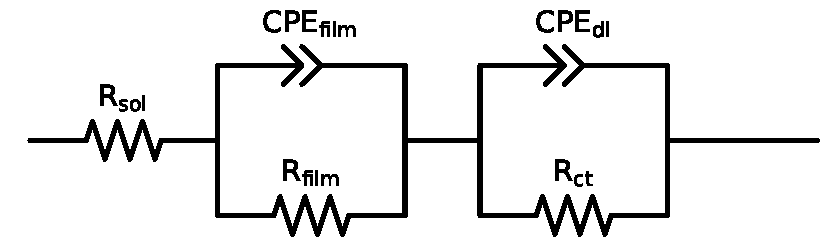
\includegraphics[width=\textwidth]{figs/2RC_voigt.pdf}
       \caption{Series configuration (Voigt) of 2RC system.}
       \label{fig:voigt}
   \end{subfigure}
   \begin{subfigure}[b]{0.48\textwidth}
       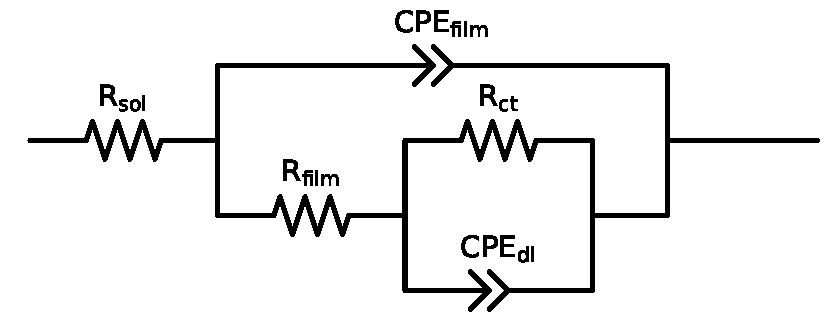
\includegraphics[width=\textwidth]{figs/2RC_nested.pdf}
       \caption{Nested configuration of 2RC system.}
       \label{fig:nested}
   \end{subfigure}
   \caption{Different configurations for 2RC systems.}
   \label{fig:2RC}
\end{figure}

$R_{\text{film}}$ plays an analogous role to $R_{\text{ct}}$ in the sense that both manifest as semicircle diameters in the Nyquist plot and both inversely reflect the degree of protection afforded at their respective interface. However, while $R_{\text{ct}}$ is a kinetic parameter governing the rate of electron transfer across the electrode/electrolyte interface, $R_{\text{film}}$ is an ionic transport parameter representing the resistance to ionic current flow both through the bulk of the film itself and through any microscopic pores and defects connecting the bulk electrolyte to the metal/film interface \cite{Kelly2002}. Just as a high $R_{\text{ct}}$ indicates sluggish interfacial reaction kinetics, a high $R_{\text{film}}$ restricts ionic transport across the film and is therefore directly associated with superior corrosion protection \cite{Lasia2014, Kelly2002}.

$C_{\text{film}}$ serves as a sensitive early indicator of coating degradation, often responding before any macroscopic evidence of corrosion becomes apparent. Its evolution is governed primarily by water uptake: upon immersion, water progressively penetrates the coating pores and, given its substantially higher dielectric constant ($\varepsilon_r \approx 80$) relative to that of a typical coating, causes a measurable increase in $C_{\text{film}}$ \cite{MetrohmEIS3, Lasia2014, Kelly2002}. A progressive increase in $C_{\text{film}}$ over time is therefore indicative of ongoing coating degradation and reduced protective performance.


\subsubsection{Warburg Element and Diffusion-Controlled Processes}

In electrochemical systems where the rate of an electrochemical reaction at the electrode surface exceeds the rate at which reactants can be supplied or products removed by diffusion, mass transport becomes the rate-limiting step \cite{Orazem2008, Barsoukov2005}. Under these conditions, a concentration gradient develops near the electrode surface, and the resulting diffusion impedance manifests in the Nyquist plot as a characteristic $45^\circ$ linear tail at low frequencies, known as the Warburg impedance \cite{Orazem2008}. In the context of aluminium alloy corrosion, this behaviour may arise at extended immersion times when diffusion of aggressive ionic species through a thickening corrosion product layer or defective coating becomes dominant \cite{Orazem2008}. In bounded systems where diffusion is confined to a finite-thickness layer, this contribution is represented by a finite-length Warburg element \cite{Barsoukov2005, Huang2018}.

\subsection{Inhibitor Efficiency from EIS Parameters} 
Electrochemical impedance spectroscopy provides a non-destructive means of quantifying the protective performance of corrosion inhibitors through the analysis of equivalent circuit parameters extracted from the impedance response \cite{Orazem2008, Lamaka2007}. The most direct indicator of inhibitor efficiency is the charge transfer resistance $R_{ct}$. Since it is inversely proportional to the corrosion current density through the Stern--Geary relation (Equation~\ref{eq:icorr}), an increase in $R_{ct}$ upon addition of an inhibitor directly reflects a reduction in the rate of anodic dissolution or cathodic reduction at active sites \cite{Revie2008, Orazem2008}. The inhibitor efficiency $\eta$ can therefore be expressed as:

\begin{equation}
    \eta = \left(1 - \frac{R_{ct,0}}{R_{ct,i}}\right) \times 100\,\%
    \label{eq:IE}
\end{equation}

where $R_{ct,0}$ and $R_{ct,i}$ are the charge transfer resistances measured in the absence and presence of the inhibitor, respectively \cite{Lamaka2007, Orazem2008}. Beyond $R_{ct}$, the double layer capacitance $C_{dl}$ provides complementary information: a decrease in $C_{dl}$ upon inhibitor addition is indicative of adsorption of inhibitor molecules at the electrode surface, which displaces the water molecules and ions previously occupying the double layer and reduces its effective dielectric permittivity \cite{Sastri2007, Orazem2008}. In systems where inhibitors are released from a reservoir such as an LDH coating, the evolution of both $R_{\text{film}}$ and $R_{ct}$ over immersion time provides a particularly informative picture: an initial decrease in $R_{\text{film}}$ due to electrolyte uptake followed by a recovery or stabilisation of $R_{ct}$ is the electrochemical signature of active inhibitor release compensating for barrier degradation \cite{BoualiReview2020, MartinezViademonte2020,Tedim2010}.

%% PERHAPS REMOVE SECTIONS RELATED TO MORE COMPLEX CIRCUITS - AT LEAST RELATED TO THE DESCRIPTION OF RFILM OR ROXIDE AND SO ON
%% ALSO REMOVE WARBURG? BUT PERHAPS IT IS IMPORTANT TO MENTION DIFFUSION AND MASS LIMIT PROCESSES?
%% DO WE NEED TO PUT INHIBITOR EFFICIENCY? ARE WE GOING TO CALCULATE IT?

\chapter{Methodology}

\section{Pre-selection of inhibitors}
\label{sec:inhibitor_selection}
As discussed in WP2, the first task of the project was to do a pre-selection of the inhibitors using electrochemical impedance spectroscopy (EIS). For this purpose bare metal substrates were sequentially polished using 120, 600, 1200 and 2500 grit sandpaper under water. After polishing, the samples were rinsed with deionized water and subsequently air-dried.

The selected corrosion inhibitors are listed in Table~\ref{tab:inhibitor}, with a standard concentration of 0.005 M, except for those with lower saturation limits. Sodium chloride (NaCl) at 0.05 M was used as the electrolyte. This concentration is commonly chosen because it provides high conductivity, resulting in low solution impedance, and allows easy comparison with existing studies. The pH of each solution was also measured prior to experimentation.

\begin{table}[htbp]
    \centering
    \small 
    \caption{Composition of the solutions for testing the effectiveness of the inhibitors and respective pH values}
    \label{tab:inhibitor}
    \begin{tabular}{@{} r l c S[table-format=1.2] @{}}
        \toprule
        No. & Solution Composition & \makecell{Concentration of\\ the reagent} & {pH} \\
        \midrule
        1 & NaCl 0.05 M                                & ---       & 7.38 \\
        2 & NaCl 0.05 M + \ce{NaVO3}                   & 0.005 M   & 7.41 \\
        3 & NaCl 0.05 M + \ce{Na2MoO4}                 & 0.005 M   & 6.70 \\
        4 & NaCl 0.05 M + 2-mercaptobenzothiazole      & Saturated & 5.67 \\
        5 & NaCl 0.05 M + benzotriazole                & 0.005 M   & 5.75 \\
        6 & NaCl 0.05 M + 8-hydroxyquinoline           & Saturated & 6.42 \\
        7 & NaCl 0.05 M + L-cysteine                   & 0.005 M   & 6.54 \\
        \bottomrule
    \end{tabular}
\end{table}

EIS measurements were then performed inside a Faraday cage using a Gamry Interface 1000 potentiostat linked to a computer and Gamry Framework v.6.33 and Echem Analyst v.6.33 software packages for data acquisition and analysis. Measurements were conducted at open circuit potential with a 10 mV sinusoidal perturbation over a frequency range of 100 kHz to 10 mHz, using 10 points per decade. For the initial measurement, the lower frequency limit was set to 100 mHz due to insufficient sample stability.

A conventional three-electrode configuration was used, comprising a saturated calomel electrode (SCE) as the RE, a platinum foil as the CE, and the exposed AC46000 substrate as the WE. The samples were immersed for a total duration of seven days, with EIS measurements collected at 0 h, 1 h, 4 h, 8 h, 24 h, 48 h, 72 h and 168 h. 

\section{Determine ECM for EIS}
\label{sec:fitting_software}
Determining an appropriate equivalent circuit model (ECM) for electrochemical impedance spectroscopy (EIS) spectra is among the most important steps in impedance analysis, as it enables the deconvolution of overlapping electrochemical processes and their quantification through physically meaningful parameters, such as charge transfer resistance ($R_{\text{ct}}$), film resistance ($R_{\text{film}}$), and double-layer capacitance ($C_{\text{dl}}$).

Despite its centrality to the analysis, ECM identification remains a laborious task. Commercial software packages such as ZView and Gamry Echem Analyst rely on nonlinear least-squares (NLLS) fitting routines, most commonly the Levenberg-Marquardt algorithm, which are inherently sensitive to the choice of initial parameter estimates \cite{GamryEISModeling,Zou2023}. While heuristic approaches exist to guide these estimates, such as reading characteristic resistances from the diameters of semicircular arcs in the Nyquist representation or extracting time constants from Bode phase plots, the process remains largely manual and iterative, demanding considerable operator experience to avoid convergence to local minima or physically unreasonable solutions.

In response to these limitations, a number of open-source, programmatic alternatives have been developed, predominantly in Python. Among these, \texttt{impedance.py} provides a flexible framework for ECM fitting and validation \cite{Murbach2020}. More recently, tools such as \texttt{AutoECM} and \texttt{AutoEIS} have incorporated machine learning methodologies into the workflow. AutoECM employs supervised classification models such as Random Forest, XGBoost (XGB), and convolutional neural network (CNN) architectures \cite{Schaeffer2023}. These are trained on libraries of previously validated circuit-spectrum pairs to predict candidate ECMs for new datasets \cite{Schaeffer2023}. AutoEIS, by contrast, adopts a probabilistic framework grounded in Bayesian inference, enabling uncertainty quantification in both circuit structure selection and parameter estimation \cite{Zhang2023}. A notable limitation shared by both tools, however, is the apparent discontinuation of active maintenance by their respective developers. As a consequence, dependency incompatibilities with more recent versions of core scientific Python libraries have rendered them largely non-functional in current environments.

Given this landscape, \texttt{impedance.py} emerges as the most viable open-source option. In its standard implementation, it operates analogously to commercial software: the user must supply the impedance dataset, an \textit{a priori} circuit string, and initial parameter guesses. Two optional fitting configurations are available. The first, \texttt{weight\_by\_modulus}, applies the modulus of the complex impedance as a frequency-dependent weighting factor which ensures that data points spanning several decades of impedance magnitude contribute proportionally to the objective function. The second, \texttt{global\_opt}, invokes a basin-hopping algorithm, which combines stochastic perturbation of parameter coordinates with local minimization and a Metropolis-type acceptance criterion to escape local minima. Importantly, \texttt{global\_opt} is incompatible with \texttt{weight\_by\_modulus} and given that EIS datasets span several decades in frequency, commonly from 10~mHz to 100~kHz, and correspondingly large ranges in impedance magnitude, modulus weighting is generally considered essential to prevent low-frequency, high-impedance data from disproportionately dominating the fit residuals. 

To overcome the dependence on user-supplied initial guesses while retaining the precision of local optimisation, a hybrid fitting framework was developed building upon \texttt{impedance.py} and the Differential Evolution (DE) algorithm. DE is a stochastic, population-based global optimisation metaheuristic well-suited to high-dimensional, non-differentiable, and multimodal objective functions \cite{Ahmad2022, Storn1997}. The algorithm evolves a population of candidate solutions across successive generations through three operators: mutation, which generates trial vectors via linear combinations of population members; crossover, which probabilistically exchanges parameter values between candidate and trial vectors; and selection, which retains whichever vector yields a lower objective function value \cite{Ahmad2022, Storn1997}. Crucially, DE requires no gradient information, making it less likely to become trapped at local minima \cite{Leite2022} and therefore particularly appropriate for the complex, rugged parameter landscapes characteristic of multi-element ECM fitting.

In the proposed workflow, the user supplies only physically motivated parameter bounds for each circuit element rather than precise initial estimates. The DE algorithm then explores this parameter space to identify the approximate order of magnitude and value of each component. To accelerate convergence, given that circuit element values typically span many orders of magnitude, the optimisation is performed in logarithmic space, transforming the search domain such that each decade is weighted uniformly. This logarithmic reparameterisation substantially improves the efficiency of the population-based search and reduces sensitivity to the scale disparity between, for example, charge-transfer resistances on the order of kilohms and double-layer capacitances on the order of microfarads.

Once the DE stage yields a sufficiently accurate global estimate, the resulting parameter vector is passed to a Nelder--Mead local optimiser, which performs a derivative-free refinement of the solution in the immediate vicinity of the global estimate. This intermediate step improves the quality of the starting point before the final refinement stage, reducing the risk of the subsequent gradient-based optimiser being misled by residual roughness in the objective function landscape. The refined parameter vector is then passed as the initial condition to the Levenberg--Marquardt local optimiser within \texttt{impedance.py}, with \texttt{weight\_by\_modulus} activated, to obtain statistically meaningful parameter estimates together with their associated uncertainties.

\section{Pre-treatments}
\label{sec:pretreatments}

As previously discussed, the presence of intermetallic particles (IMPs) on the surface of the aluminium alloy can negatively affect LDH growth homogeneity and must therefore be removed prior to coating deposition. Two pre-treatment procedures were evaluated alongside a reference polished condition, and for selected specimens an additional anodising step was subsequently applied. To assess the effectiveness of each pre-treatment, scanning electron microscopy (SEM) and energy dispersive X-ray spectroscopy (EDS) analyses were conducted on the treated surfaces, with the objective of identifying which IMPs remained and determining which pre-treatment was most conducive to homogeneous LDH growth.

\subsection{Chemical Pre-treatment}
\label{subsec:chemical_pretreatment}

The chemical pre-treatment consisted of alkaline cleaning in a \qty{0.1}{\molar} \ce{NaOH} solution at room temperature for \qty{120}{\second}, followed by acid pickling in a \qty{0.1}{\molar} \ce{HNO3} solution for \qty{480}{\second}. Each step was followed by rinsing with deionised water, and the specimens were finally dried in air.

\subsection{Industrial Pre-treatment}
\label{subsec:industrial_pretreatment}

The industrial pre-treatment followed a multistep protocol. Degreasing was performed in Metaclean T2001 (an alkaline cleaner based on metal silicates with complexing and surface-active agents) at a concentration of \qty{48}{\gram\per\liter} and approximately \qty{65}{\degreeCelsius} for \qty{10}{\minute}. Although the recommended immersion time is \qty{25}{\minute}, a shorter duration was deemed sufficient given that no oils or lubricants were employed during specimen preparation. Following rinsing with deionised water, the specimens were alkaline etched in Turco Liquid Aluminetch N2 (a sodium hydroxide and phosphate-based solution) at \qty{38}{\gram\per\liter} and \qty{65}{\degreeCelsius} for \qty{45}{\second}, and subsequently rinsed with deionised water. Desmutting was then carried out in Turco Liquid Smutgo NC (a formulation based on ferric sulfate, nitric acid, sodium hydrogendifluoride, and sulfuric acid) at a concentration of \qty{180}{\milli\liter\per\liter} and \qty{30}{\degreeCelsius} for approximately \qty{5}{\minute}, before a final rinse with deionised water and drying in air.

\subsection{Anodising}
\label{subsec:anodising}

For selected specimens, a tartaric-sulphuric acid (TSA) anodising step was carried out following the industrial pre-treatment, prior to LDH synthesis. The anodising bath consisted of \qty{10}{\gram\per\liter} tartaric acid and \qty{10}{\gram\per\liter} sulphuric acid at a temperature of \qty{20}{\degreeCelsius}. An AA1050 aluminium alloy plate was used as the cathode. A voltage of \qty{14}{\volt} was applied for \qty{2}{\minute}, after which the specimens were rinsed with deionised water and dried in air prior to LDH synthesis.

\section{LDH Synthesis}
\label{sec:LDH_synthesis}

To assess the influence of the pre-treatment on LDH growth, films were grown on three sets of specimens: those subjected to the chemical pre-treatment, those subjected to the industrial pre-treatment, and mechanically polished reference specimens. In all cases, the same in situ hydrothermal synthesis procedure was employed to ensure comparability.

The synthesis solution was prepared by first dissolving \ce{NH4NO3} at a concentration of \qty{0.6}{\molar} in \qty{600}{\milli\liter} of deionised water (resistivity \qty{18}{\mega\ohm\centi\meter}) under magnetic stirring. The pH of this solution was measured and found to be below 5. \ce{Zn(NO3)2.6H2O} was then added at a concentration of \qty{0.1}{\molar}, together with an additional \qty{300}{\milli\liter} of deionised water. The pH was subsequently adjusted to $6.5 \pm 0.1$ using a 5\% ammonia solution. Deionised water was then added to bring the total volume to \qty{1}{\liter}, and the pH was measured and corrected to $6.5 \pm 0.1$ if required.

For LDH film growth, \qty{300}{\milli\liter} of the synthesis solution was transferred to a vessel and pre-heated to \qty{95}{\degreeCelsius}, sufficient for the simultaneous immersion of three specimens. The specimens were suspended vertically and fully immersed in the solution for \qty{1}{\hour} under magnetic stirring. Upon completion, the specimens were removed, rinsed with deionised water, and dried with compressed air.

To characterise the LDH films and compare growth across the different substrate conditions, X-ray diffraction (XRD) analysis was conducted. From the diffraction patterns, the basal spacing ($d_{003}$) was determined using Bragg's law, providing structural confirmation of LDH formation and enabling comparison of film crystallinity across the different pre-treatment conditions.

\section{Inhibitor Incorporation}
\label{sec:inhibitor_incorporation}

Based on the screening results presented in Section~\ref{sec:results_inhibitor_selection}, the three most promising inhibitor systems were selected for intercalation into the LDH interlayer galleries.

To incorporate \ce{NaVO3} and L-cysteine into the LDH interlayer galleries, anion exchange was performed by immersing the as-grown LDH films in a \qty{0.1}{\molar} inhibitor solution at \qty{25}{\degreeCelsius} for \qty{3}{\hour}. Following this, the specimens were rinsed with deionised water and dried with compressed air.

For MBT incorporation, \ce{NaOH} was added at a concentration of \qty{0.1}{\molar} to a \qty{0.1}{\molar} MBT solution to deprotonate the molecule into its anionic form (\ce{MBT^-}), which is required for both solubility and intercalation into the LDH galleries \cite{}. Given the amphoteric nature of aluminium and its susceptibility to alkaline dissolution (Section~\ref{sec:pourbaix}), the pH was adjusted to 10.2 using a \qty{1}{\molar} \ce{NaOH} solution. To minimise the risk of surface attack, the immersion time was limited to \qty{30}{\minute} with visual inspection at \qty{10}{\minute} intervals, after which the specimens were rinsed with deionised water and dried with compressed air.

To verify the successful intercalation of the corrosion inhibiting anions, the specimens were subjected to X-ray diffraction (XRD) analysis. A shift in the characteristic $2\theta$ reflection angles relative to the as-grown LDH films would indicate a change in the basal spacing ($d_{003}$) and consequently in the interlayer gallery height, confirming the incorporation of guest anions into the LDH interlayer space.

\section{Evaluation of Corrosion Performance}
\label{sec:corrosion_evaluation}

Following successful inhibitor intercalation, the corrosion performance of the LDH-based coatings was evaluated by immersing the specimens in a \qty{0.05}{\molar} \ce{NaCl} solution and conducting electrochemical impedance spectroscopy (EIS) measurements, following the procedure described in Section~\ref{sec:inhibitor_selection}. The resulting spectra were fitted using the software developed in Section~\ref{sec:fitting_software}, and the extracted $R_{\text{ct}}$ and $C_{\text{dl}}$ values were compared across the different inhibitor systems to assess their relative corrosion protection performance. In addition, the specimens were examined optically for visual evidence of corrosion, and potentiodynamic polarisation (PDP) measurements were conducted to complement the impedance analysis.

\section{Top Coating and Complex Geometries}
\label{sec:topcoat}

Once inhibitor intercalation and corrosion performance had been established, a water-based polyurethane colloidal formulation (supplied by CIDETEC, Spain) was applied to the inhibitor-intercalated planar specimens via anodic  electrodeposition. In this process, the negatively charged colloidal particles  dispersed in the aqueous bath migrate under the applied electric field towards  the anodically polarised substrate, where a localised increase in pH at the  anode surface --- caused by water oxidation --- triggers particle coagulation and film formation. The specimens were immersed in the polyurethane bath and a voltage of \qty{80}{\volt} was applied for \qty{1}{\minute} at room temperature. Following deposition, the specimens were allowed to dry in air for approximately \qty{30}{\minute} prior to curing in an oven at \qty{120} {\degreeCelsius} for \qty{1}{\hour}. 

To evaluate the adhesion and microstructural integrity of the complete multilayer system, cross-sections of the coated planar specimens were prepared by cutting and examined by SEM and EDS analysis. EDS elemental mapping was conducted to assess the distribution of target elements across the multilayer cross-section and to evaluate the degree of interpenetration between the organic topcoat and the underlying LDH conversion coating. Coating thickness was additionally measured using an Elcometer gauge on both planar and complex geometry specimens.

\chapter{Results and Discussion}

\section{Pre-selection of Inhibitors}
\label{sec:results_inhibitor_selection}

In the first part of this work, a pre-selection of corrosion inhibitors was conducted based on EIS measurements. The impedance spectra acquired at \qty{1}{\hour} and \qty{168}{\hour} of immersion are presented in Figures~\ref{fig:inhibitors_bode} and~\ref{fig:inhibitors_nyquist}.

\begin{figure}[H]
   \centering
   % Linha 1
   \begin{subfigure}[b]{0.95\textwidth}
       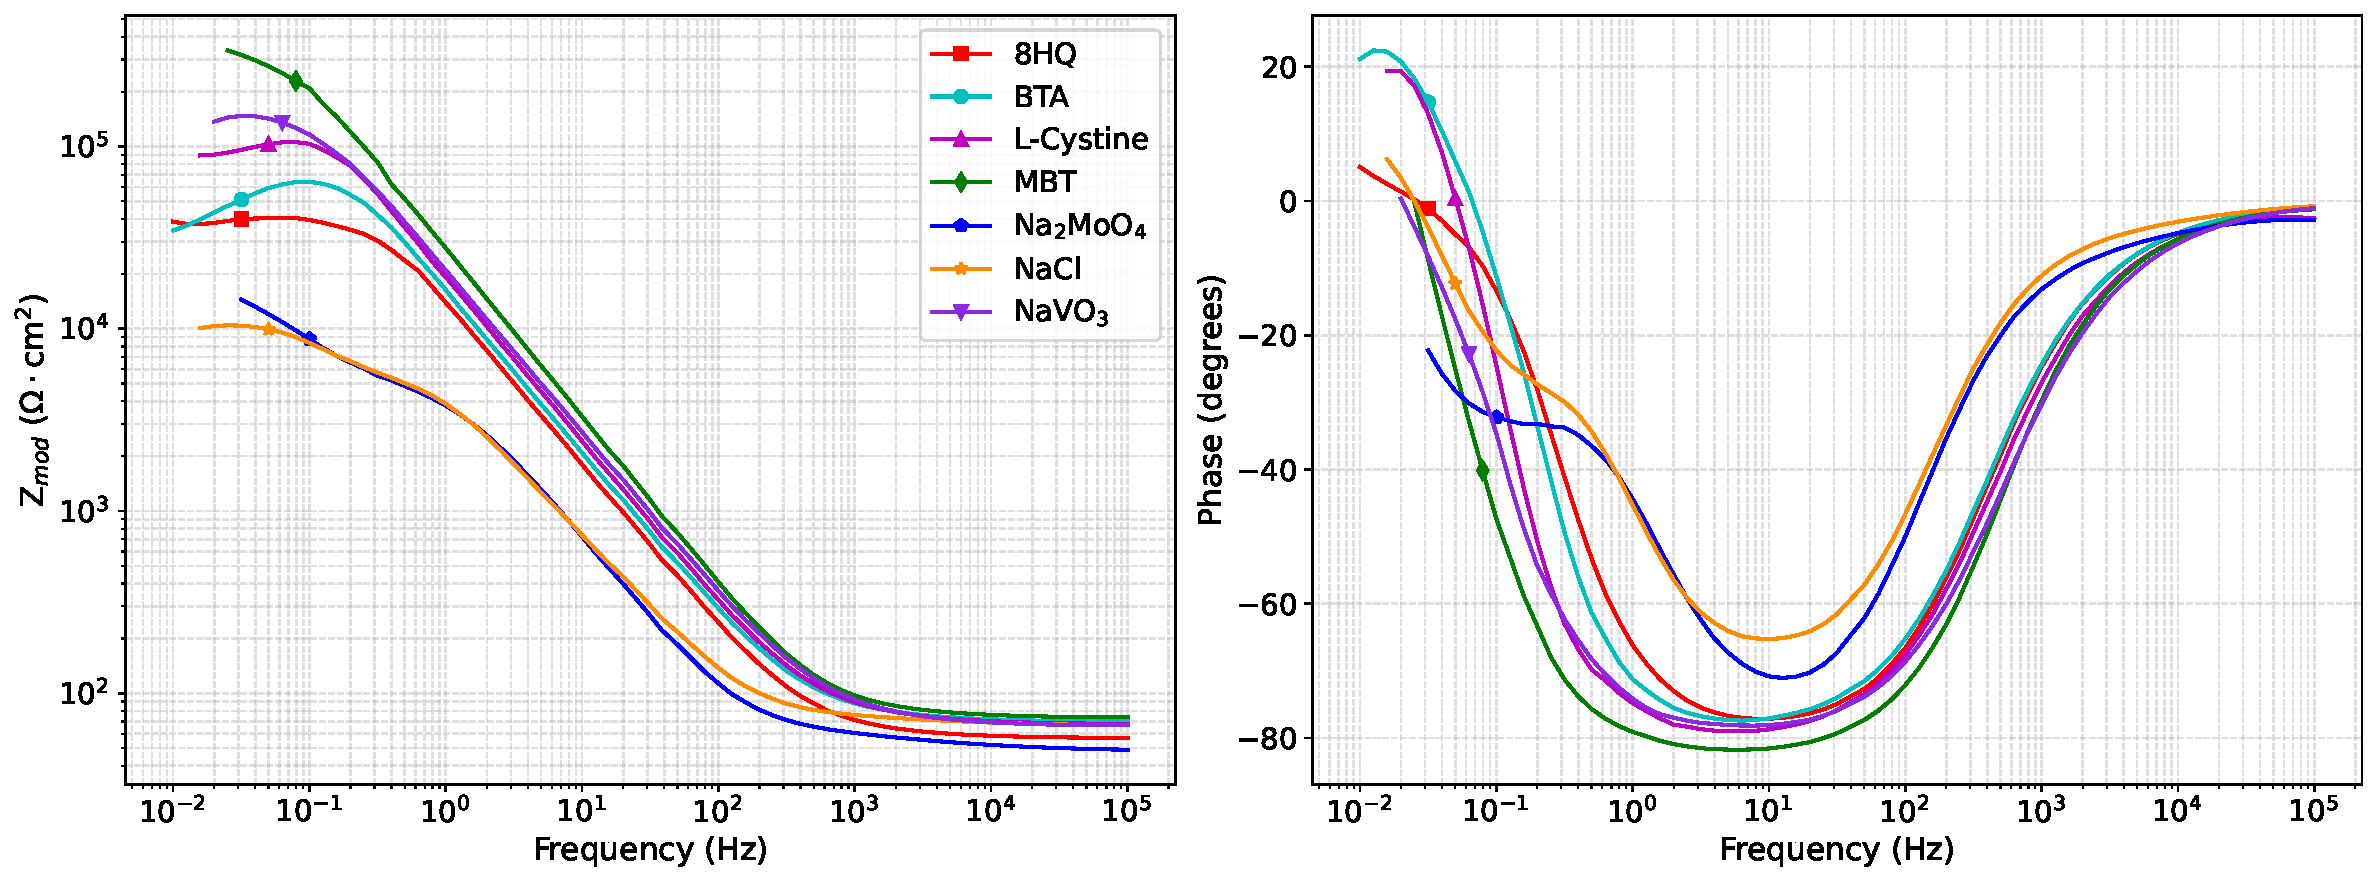
\includegraphics[width=\textwidth]{figs/bode_1H_inhibitors.pdf}
       \caption{1H bode}
       \label{fig:inhibitors_1h_bode}
   \end{subfigure}

   \vspace{0.5cm}

   \begin{subfigure}[b]{0.95\textwidth}
       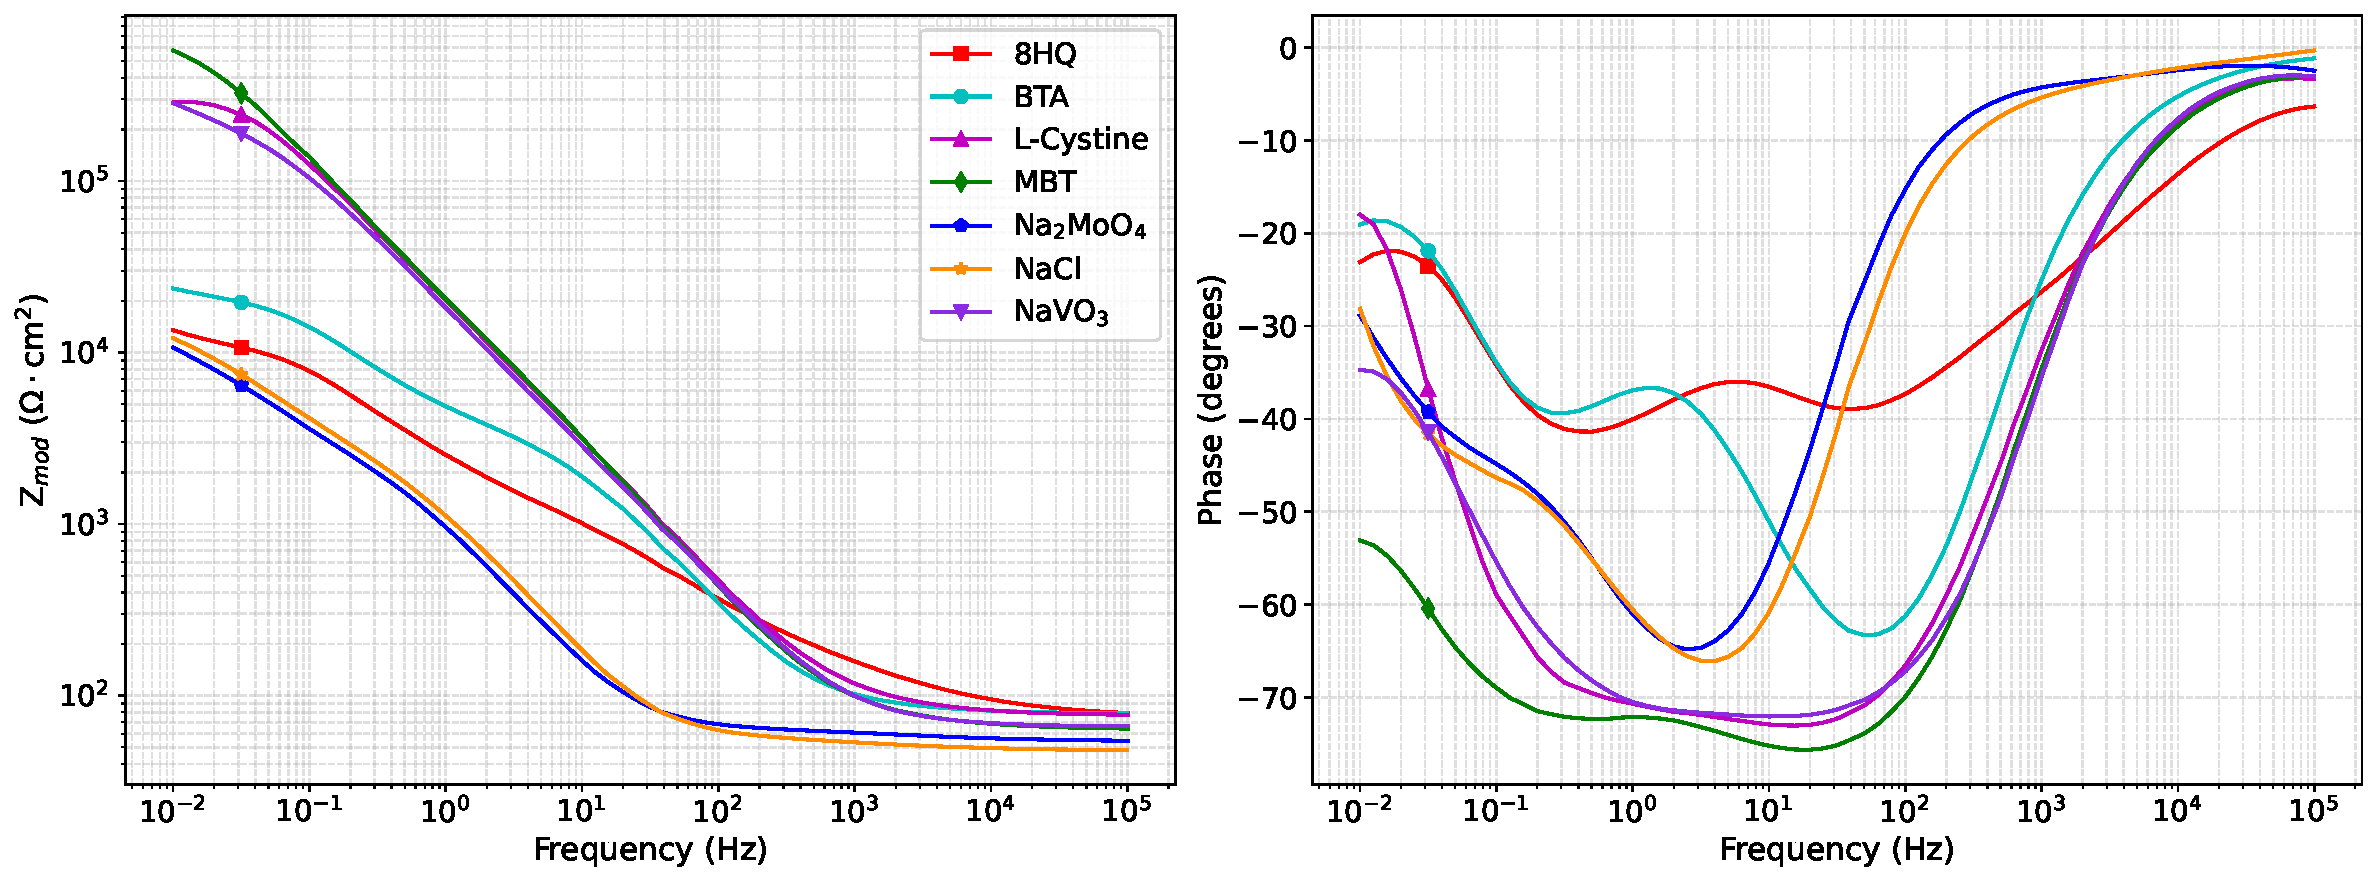
\includegraphics[width=\textwidth]{figs/bode_168H_inhibitors.pdf}
       \caption{168H bode}
       \label{fig:inhibitors_168h_bode}
   \end{subfigure}
   \caption{Bode spectra for 1h immersion.}
   \label{fig:inhibitors_bode}
\end{figure}

\begin{figure}[H]
   \centering
   \begin{subfigure}[b]{0.4\textwidth}
       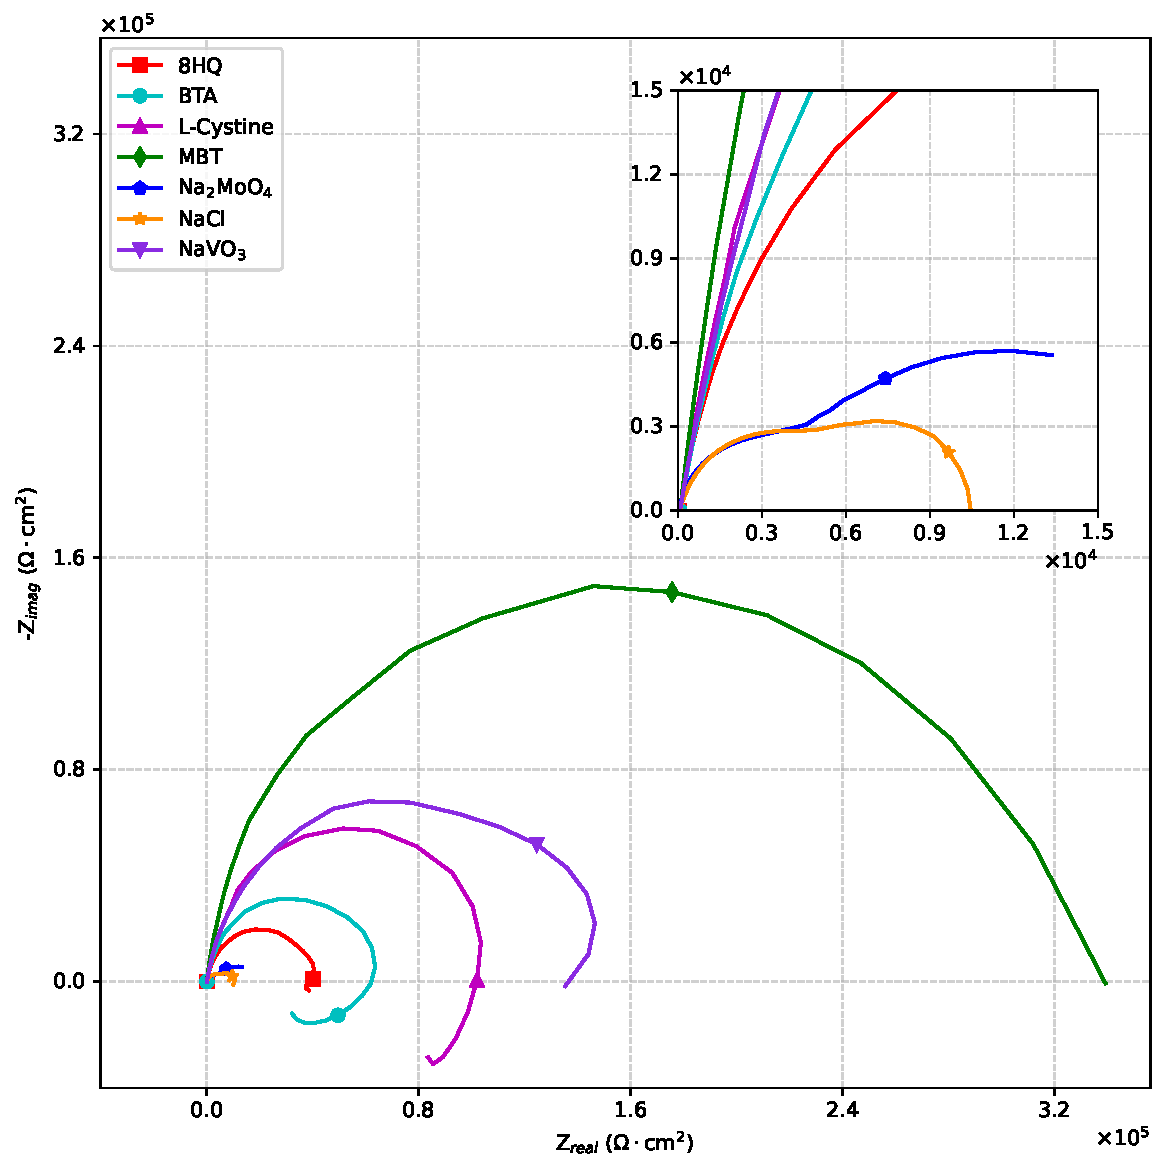
\includegraphics[width=\textwidth]{figs/nyquist_1H_inhibitors.pdf}
       \caption{1H nyquist}
       \label{fig:inhibitors_1h_nyquist}
   \end{subfigure}
   \begin{subfigure}[b]{0.4\textwidth}
       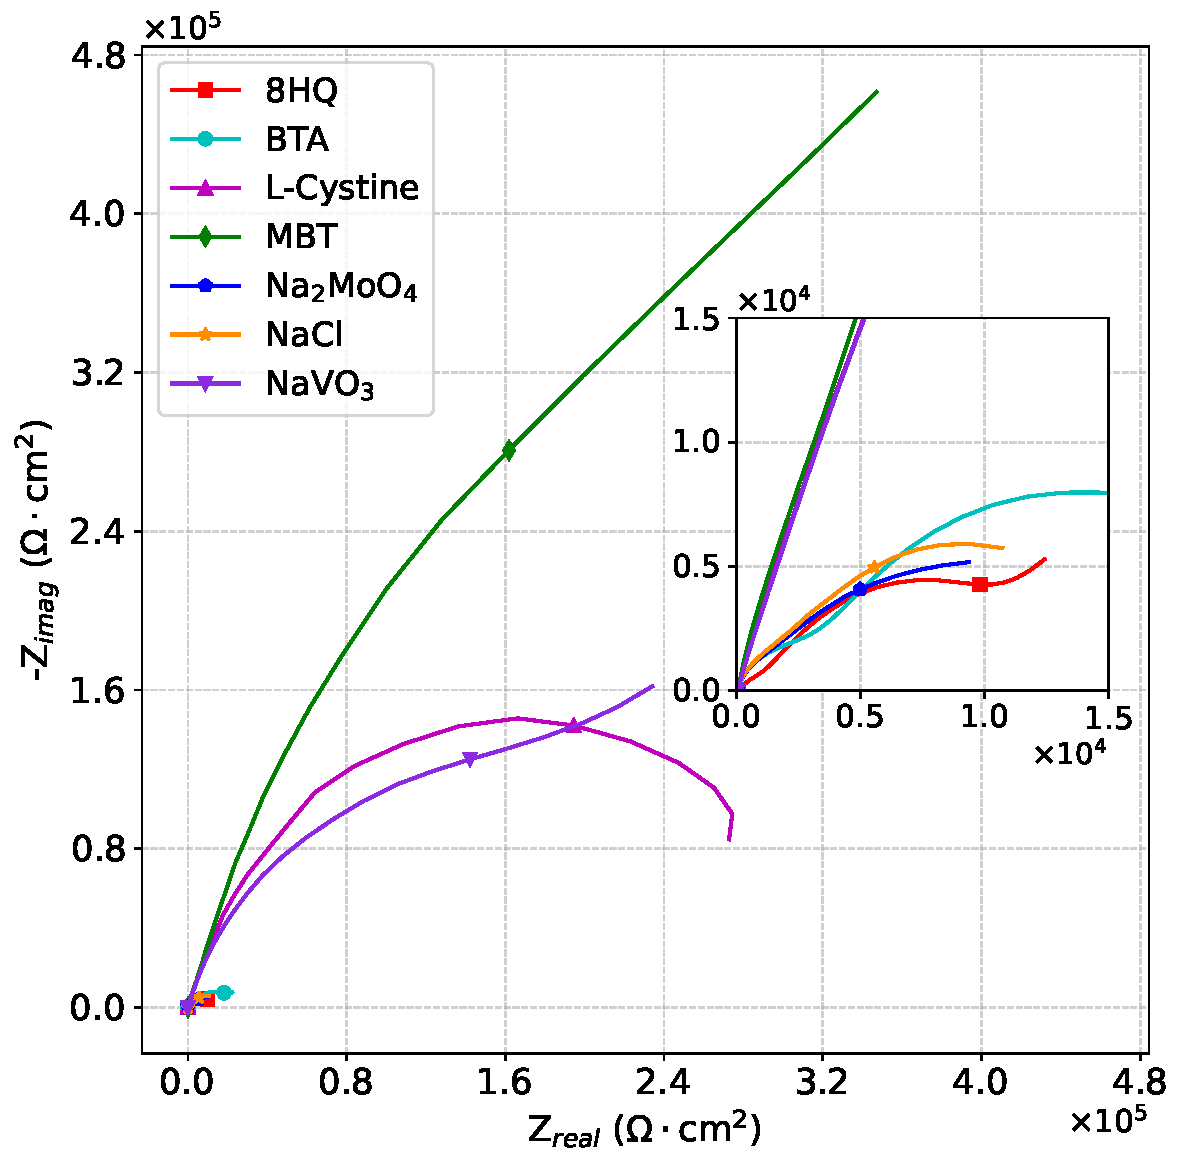
\includegraphics[width=\textwidth]{figs/nyquist_168H_inhibitors.pdf}
       \caption{168H nyquist}
       \label{fig:inhibitors_168h_nyquist}
   \end{subfigure}   
   \caption{Nyquist spectra for 1h immersion.}
   \label{fig:inhibitors_nyquist}
\end{figure}

As can be observed in the Nyquist plots (Figures~\ref{fig:inhibitors_1h_nyquist} and~\ref{fig:inhibitors_168h_nyquist}), MBT, \ce{NaVO3}, and L-cysteine exhibit the highest low-frequency impedance magnitudes at both immersion times, indicative of superior inhibition performance. Furthermore, the impedance response of these three inhibitors increases progressively with immersion time, suggesting that their protective action is not merely passive but involves an active reinforcement of the surface film, likely through continued adsorption or the formation of insoluble surface complexes over the course of the experiment. This trend is corroborated by the Bode plots (Figures~\ref{fig:inhibitors_1h_bode} and~\ref{fig:inhibitors_168h_bode}), in which the same three systems consistently exhibit the largest semicircle diameters, reflecting elevated charge-transfer resistance values.

To validate these observations quantitatively, spectral fitting using the software developed in Section~\ref{sec:fitting_software} was performed to evaluate the evolution of $R_{\text{ct}}$ and $C_{\text{dl}}$ over the full immersion period. The results are presented in Figure~\ref{fig:Rct_Cdl_evolution_inhibitors}.

\begin{figure}[H]
    \centering
    
\includegraphics[width=0.95\textwidth]{figs/Rct_Cdl_evolution_inhibitors.pdf} 

    \caption{Rct and Cdl evolution over time.}
    
    \label{fig:Rct_Cdl_evolution_inhibitors}
\end{figure}

The extracted parameters confirm the trends identified from visual inspection of the spectra. MBT, \ce{NaVO3}, and L-cysteine all attained $R_{\text{ct}}$ values in excess of \qty{100}{\kilo\ohm}, substantially higher than those of the remaining systems. The progressive increase in $R_{\text{ct}}$ with immersion time for these three inhibitors further supports the hypothesis of active and durable film formation at the electrode surface. Sodium molybdate, by contrast, performed comparably to the blank NaCl solution throughout the entire immersion period, with $R_{\text{ct}}$ values consistently in the range of \qtyrange{3}{4}{\kilo\ohm}. This near-complete absence of inhibition under open-circuit conditions is consistent with the known mechanism of molybdate, which requires anodic polarisation to form a protective surface film and therefore provides negligible protection in the context of free immersion in dilute NaCl \cite{Sastri2007, Vargel2020}. BTA and 8-HQ exhibited intermediate behaviour, with $R_{\text{ct}}$ values approximately between \qty{10}{\kilo\ohm} and \qty{30}{\kilo\ohm}, significantly lower than the three best-performing inhibitors.

The double-layer capacitance data further support and refine these conclusions. Sodium molybdate again showed behaviour closely resembling that of the blank NaCl system, with $C_{\text{dl}}$ values approaching \qty{100}{\micro\farad}, consistent with an essentially unprotected electrode surface. Although BTA and 8-HQ displayed relatively low initial $C_{\text{dl}}$ values, suggesting that some degree of initial adsorption does occur, these increased rapidly with immersion time, eventually converging towards values comparable to the uninhibited system. This behaviour indicates that while both inhibitors adsorb at the electrode surface in the early stages of immersion, they fail to maintain a stable protective film over time. The progressive desorption or displacement of the inhibitor allows water molecules and electrolyte ions to repopulate the double layer; given the substantially higher dielectric constant of water ($\varepsilon_r \approx 80$) relative to that of adsorbed organic species, this ingress drives $C_{\text{dl}}$ towards values characteristic of an unprotected surface \cite{Orazem2008, Sastri2007}. In contrast, MBT, L-cysteine, and \ce{NaVO3} maintained $C_{\text{dl}}$ values in the order of \qty{10}{\micro\farad} throughout the experiment, consistent with stable inhibitor adsorption, the sustained exclusion of water and electrolyte from the double layer region, and a durable reduction in interfacial reactivity, as discussed in Section~\ref{sec:double_layer}.

Using the equation~\ref{eq:IE}, the efficiency of the different inhibitors was calculated and the values are presented in table~\ref{tab:IE}.

\begin{table}[htbp]
    \centering
    \small
    \caption{Inhibition efficiency ($\eta$) of various chemical compounds extracted from electrochemical parameters.}
    \label{tab:IE}
    \begin{tabular}{@{} l c @{}}
        \toprule
        Inhibitor & Efficiency (\%) \\
        \midrule
        \ce{NaVO3}    & $98.73$ \\
        L-cystine     & $96.93$ \\
        MBT           & $96.27$ \\
        BTA           & $86.55$ \\
        8HQ           & $76.07$ \\
        Molybdate     & $1.76$  \\
        \bottomrule
    \end{tabular}
\end{table}

Optical inspection of the specimen surfaces following \qty{168}{\hour} of immersion provides complementary visual evidence of the electrochemical trends described above. The photographs are presented in Figure~\ref{fig:optical_inhibitors}.



\begin{figure}[htbp]
    \centering
    \begin{subfigure}[b]{0.20\textwidth}
        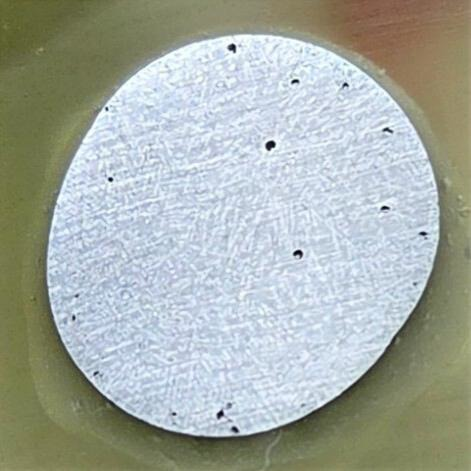
\includegraphics[width=\textwidth]{figs/optical_inhibitors/before.jpg}
        \caption{Before}
        \label{fig:optical_before}
    \end{subfigure}
    \hfill
    \begin{subfigure}[b]{0.20\textwidth}
        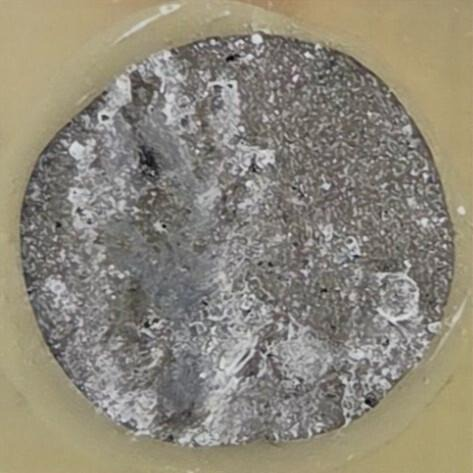
\includegraphics[width=\textwidth]{figs/optical_inhibitors/Uninhibited.jpg}
        \caption{Control}
        \label{fig:optical_control}
    \end{subfigure}
    \hfill
    \begin{subfigure}[b]{0.20\textwidth}
        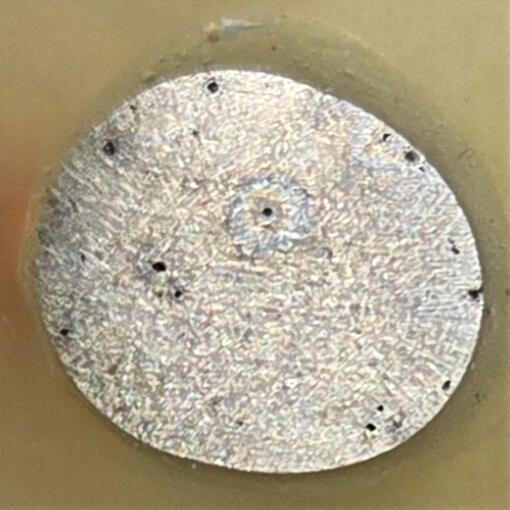
\includegraphics[width=\textwidth]{figs/optical_inhibitors/MBT.jpg}
        \caption{MBT}
        \label{fig:optical_MBT}
    \end{subfigure}
    \hfill
    \begin{subfigure}[b]{0.20\textwidth}
        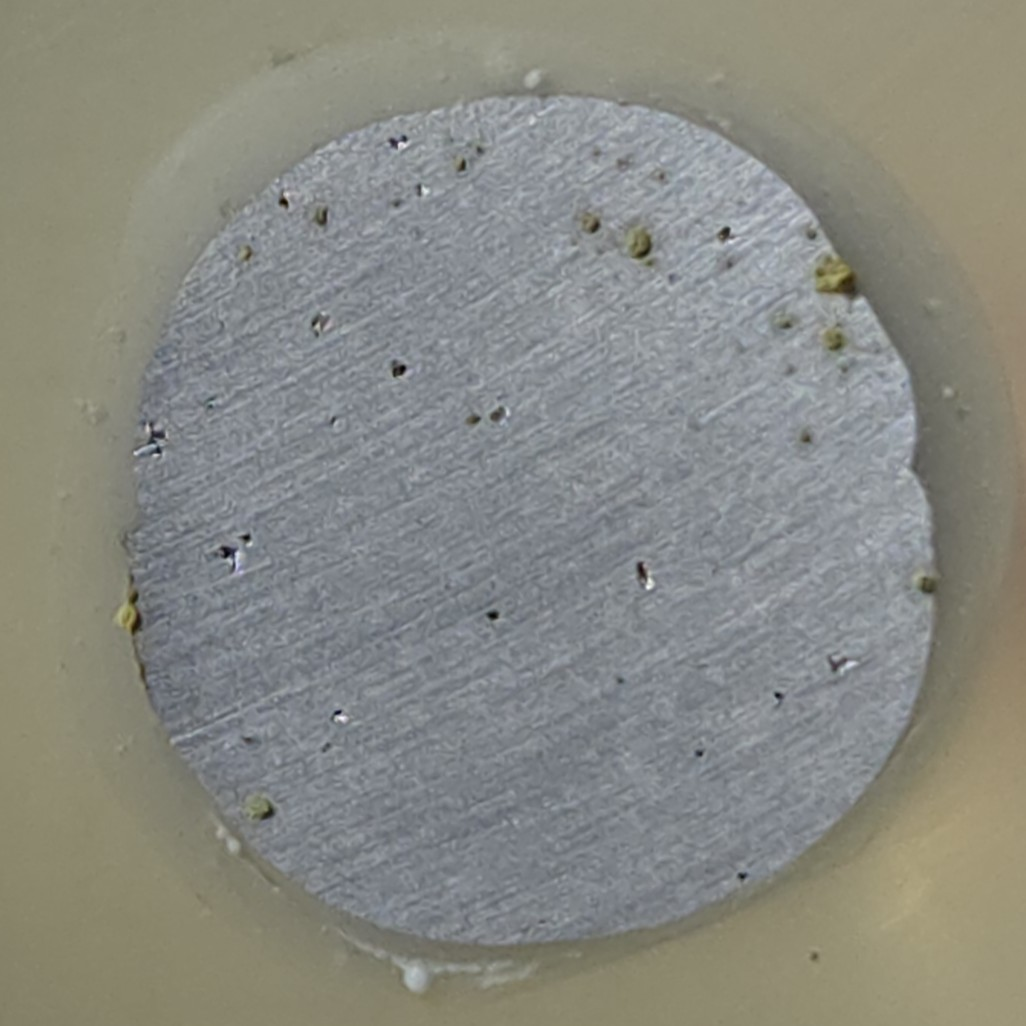
\includegraphics[width=\textwidth]{figs/optical_inhibitors/NaVO3.jpg}
        \caption{\ce{NaVO3}}
        \label{fig:optical_NaVO3}
    \end{subfigure}

    \vspace{0.3cm}

    \begin{subfigure}[b]{0.20\textwidth}
        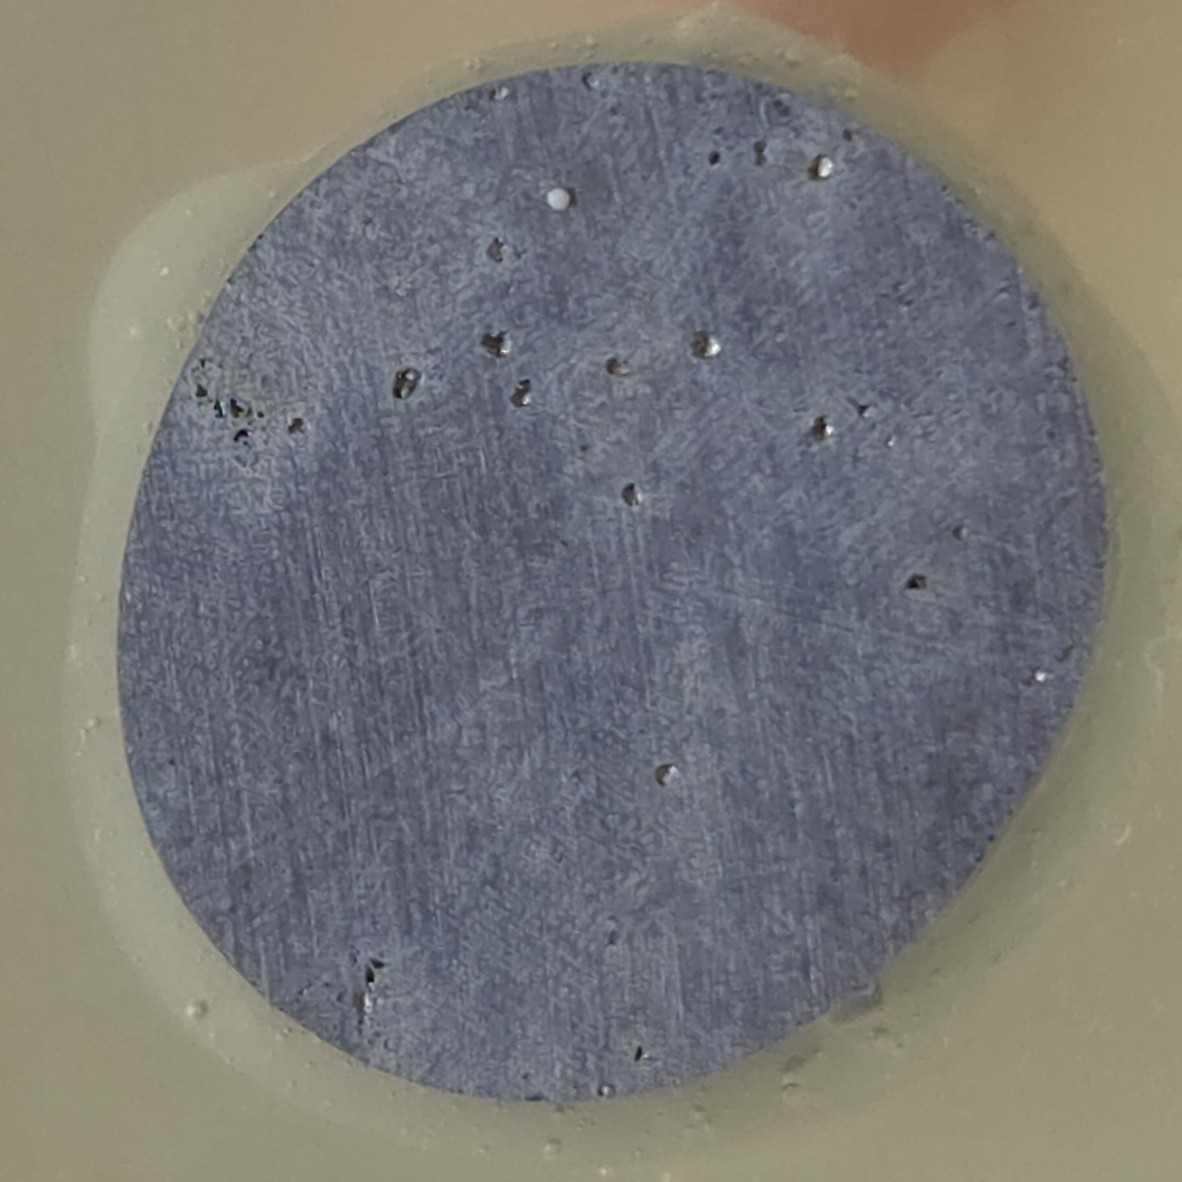
\includegraphics[width=\textwidth]{figs/optical_inhibitors/Lcysteine.jpg}
        \caption{L-cysteine}
        \label{fig:optical_Lcysteine}
    \end{subfigure}
    \hfill
    \begin{subfigure}[b]{0.20\textwidth}
        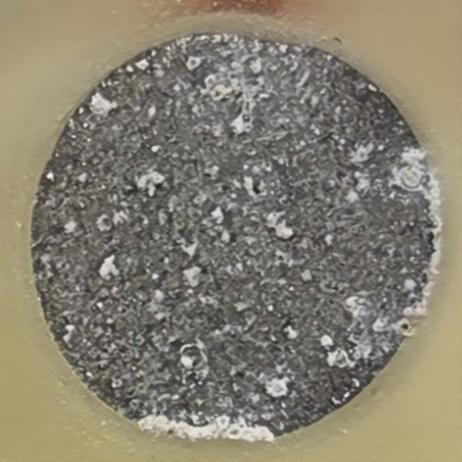
\includegraphics[width=\textwidth]{figs/optical_inhibitors/Molybdate.jpg}
        \caption{\ce{Na2MoO4}}
        \label{fig:optical_molybdate}
    \end{subfigure}
    \hfill
    \begin{subfigure}[b]{0.20\textwidth}
        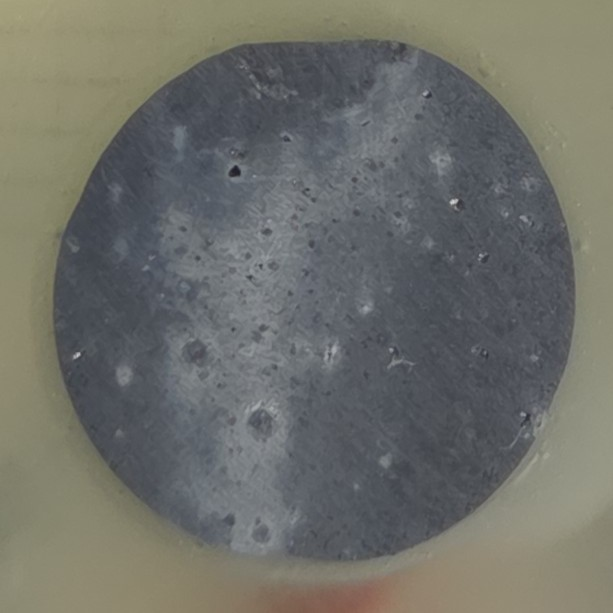
\includegraphics[width=\textwidth]{figs/optical_inhibitors/BTA.jpg}
        \caption{BTA}
        \label{fig:optical_BTA}
    \end{subfigure}
    \hfill
    \begin{subfigure}[b]{0.20\textwidth}
        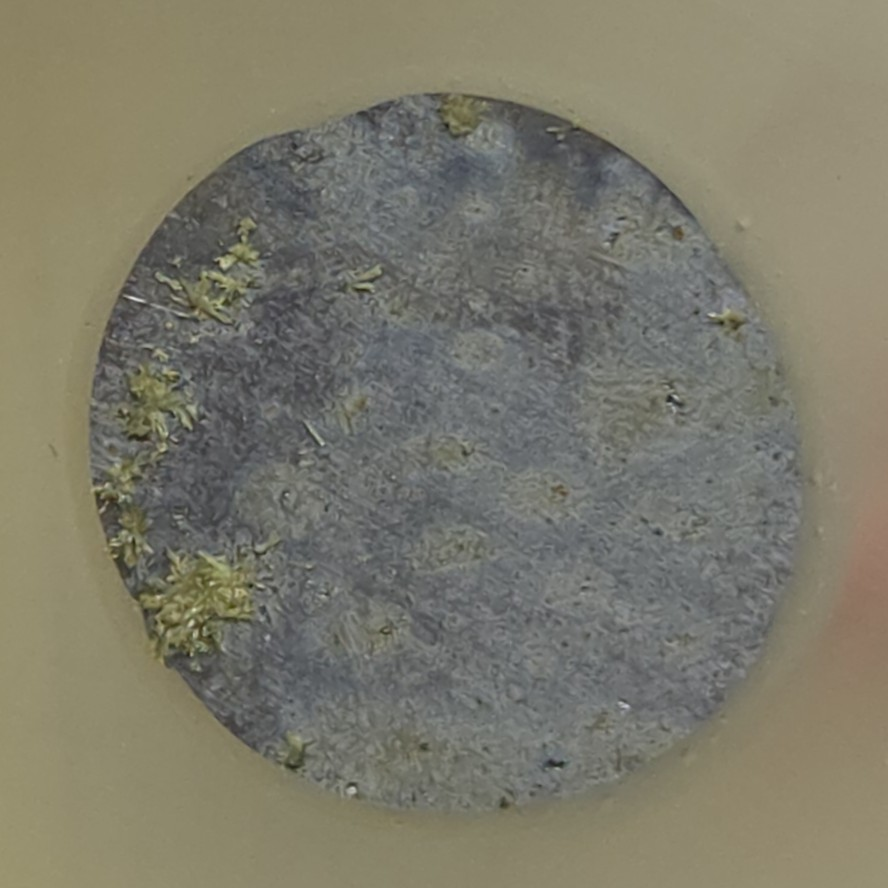
\includegraphics[width=\textwidth]{figs/optical_inhibitors/8HQ.jpg}
        \caption{8-HQ}
        \label{fig:optical_8HQ}
    \end{subfigure}
    \caption{Optical photographs of specimen surfaces following \qty{168}{\hour} 
    of immersion in \qty{0.05}{\molar} \ce{NaCl} for all inhibitor systems.}
    \label{fig:optical_inhibitors}
\end{figure}

The specimen immersed in the blank \ce{NaCl} solution (control) exhibits extensive and generalised surface degradation, serving as a reference for the uninhibited corrosion behaviour of the alloy. Among the inhibitor systems, MBT demonstrates the most effective protection, with only a single visible pit discernible from the localised discolouration of the surrounding surface --- a finding consistent with its superior $R_{\text{ct}}$ and $C_{\text{dl}}$ performance. \ce{NaVO3} ranks second, showing no visible pitting but a small number of localised yellowish deposits, attributable to the precipitation of vanadate oxides over incipient pit sites, which is indicative of active inhibitor release and localised repassivation. L-cysteine performs comparably, exhibiting no discrete pits but a diffuse whitish surface appearance characteristic of mild generalised aluminium matrix corrosion, suggesting that while localised attack is suppressed, uniform surface oxidation is not entirely prevented.

BTA and 8-HQ display intermediate levels of degradation, consistent with their moderate $R_{\text{ct}}$ values. The BTA specimen shows both discrete pitting and areas of pronounced generalised corrosion. The 8-HQ specimen similarly exhibits generalised surface corrosion alongside multiple large green-yellowish deposits, attributable to oxide or hydroxide compounds formed through interaction of the 8-HQ ligand with dissolved metal ions at pit sites, indicating that significant localised corrosion had occurred beneath these deposits despite some degree of inhibitor activity.

Sodium molybdate presents the most severely degraded surface among the inhibited specimens, with an appearance closely resembling that of the control sample and exhibiting heavy generalised corrosion. This is fully consistent with the electrochemical data, which showed molybdate to provide essentially no inhibition under free immersion conditions in dilute \ce{NaCl}.

Based on these results, MBT, \ce{NaVO3}, and L-cysteine were identified as the best-performing inhibitors among those evaluated and were therefore selected for subsequent incorporation into the ZnAl--LDH coating system.

\section{Pre-treatments}
\label{sec:results_pretreatments}

To identify the most suitable pre-treatment for LDH growth, SEM and EDSanalyses were conducted on specimens subjected to the chemical pre-treatment, the industrial pre-treatment, and mechanical polishing, the latter serving as a reference condition. The results are presented in Figures~\ref{fig:sem_eds_I} to~\ref{fig:sem_eds_III}.

\begin{figure}[htbp]
   \centering
   \begin{subfigure}[b]{0.24\textwidth}
       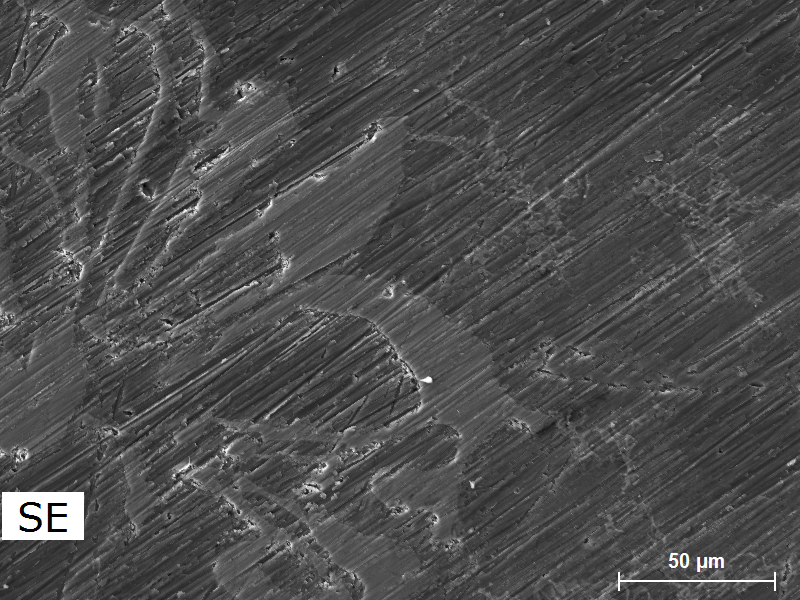
\includegraphics[width=\textwidth]{figs/I/SE_SE.png}
       \caption{SEM}
       \label{fig:sem_I}
   \end{subfigure}
   \hfill
   \begin{subfigure}[b]{0.24\textwidth}
       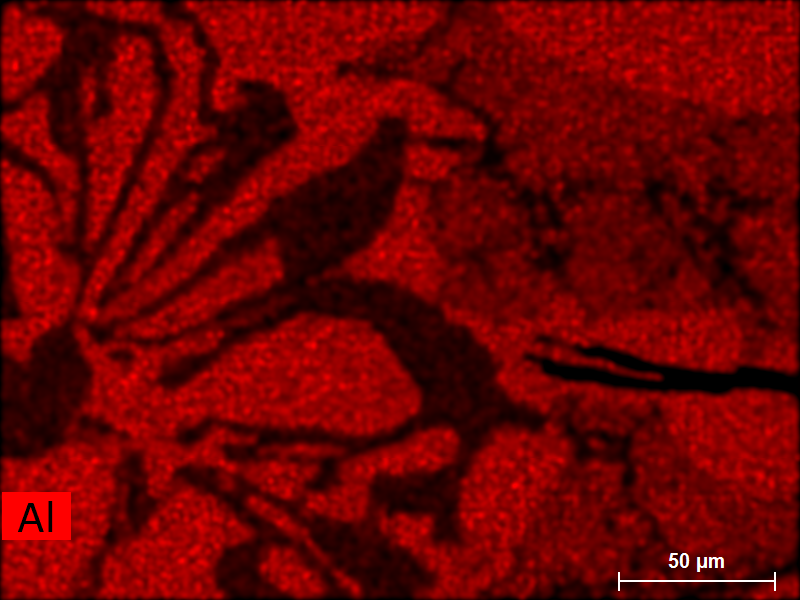
\includegraphics[width=\textwidth]{figs/I/SE_Al.png}
       \caption{Al}
       \label{fig:Al_I}
   \end{subfigure}   
   \hfill
   \begin{subfigure}[b]{0.24\textwidth}
       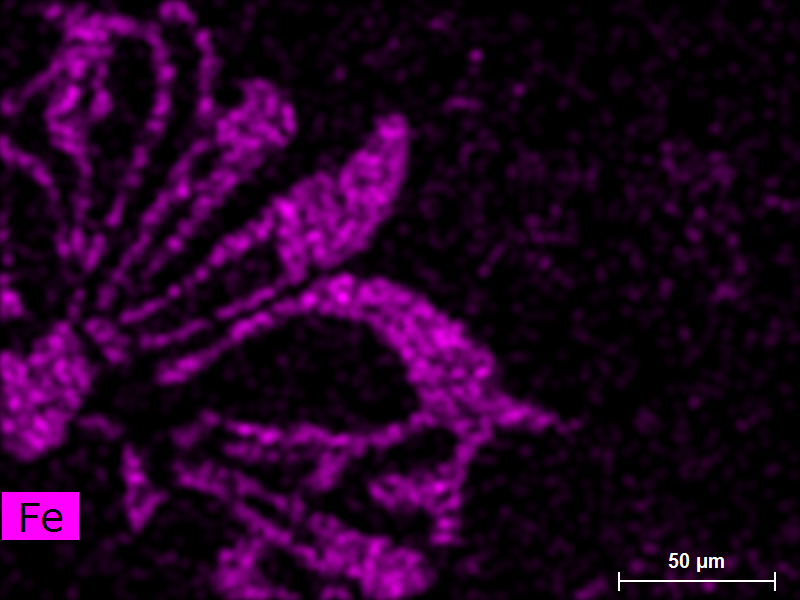
\includegraphics[width=\textwidth]{figs/I/SE_Fe.png}
       \caption{Fe}
       \label{fig:Fe_I}
   \end{subfigure}
   \hfill
   \begin{subfigure}[b]{0.24\textwidth}
       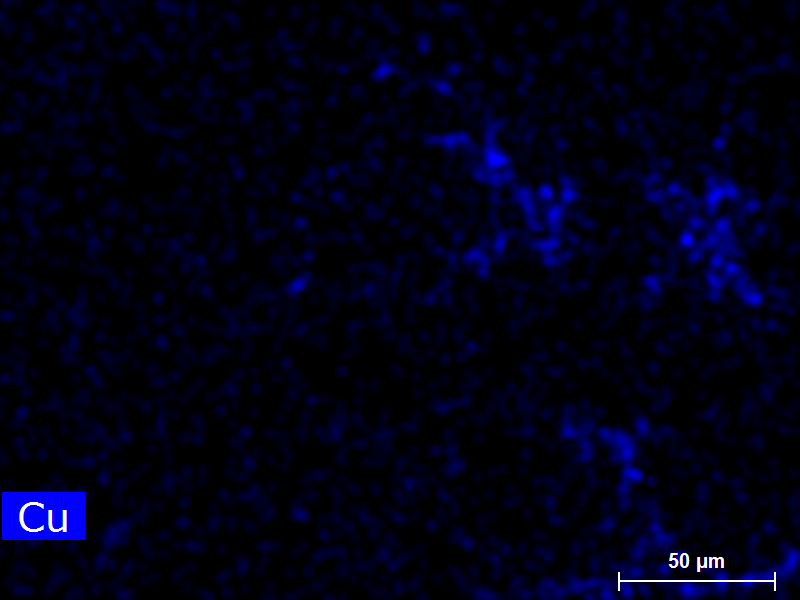
\includegraphics[width=\textwidth]{figs/I/SE_Cu.png}
       \caption{Cu}
       \label{fig:Cu_I}
   \end{subfigure}
   \begin{subfigure}[b]{0.24\textwidth}
       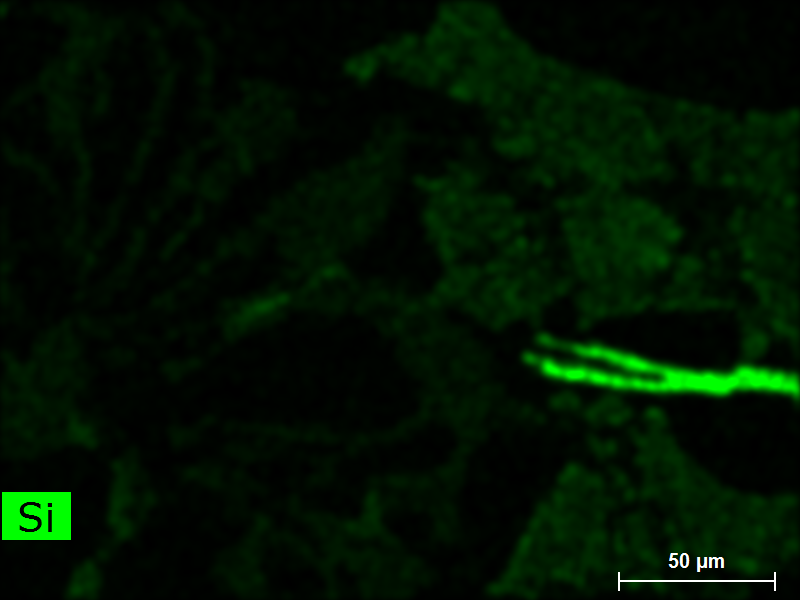
\includegraphics[width=\textwidth]{figs/I/SE_Si.png}
       \caption{Si}
       \label{fig:Si_I}
   \end{subfigure}
   \hfill
   \begin{subfigure}[b]{0.24\textwidth}
       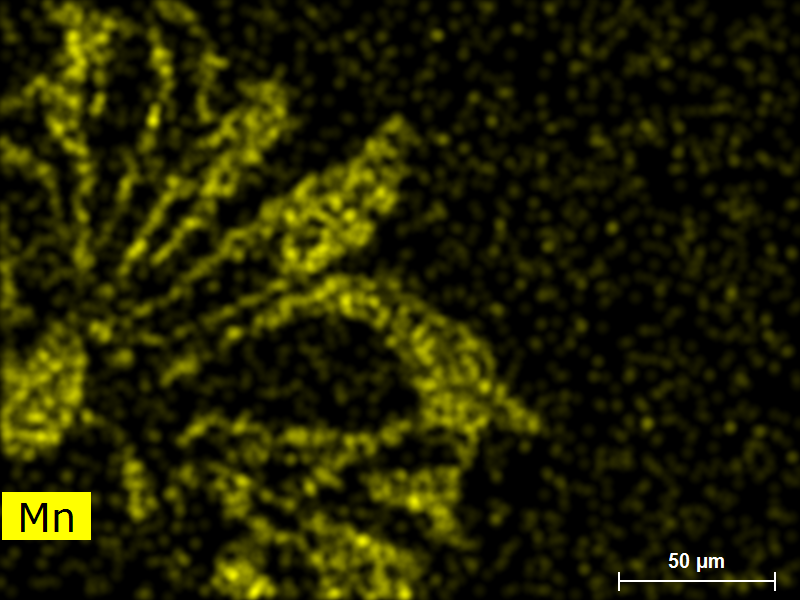
\includegraphics[width=\textwidth]{figs/I/SE_Mn.png}
       \caption{Mn}
        \label{fig:Mn_I}
    \end{subfigure}
    \hfill
    \begin{subfigure}[b]{0.24\textwidth}
        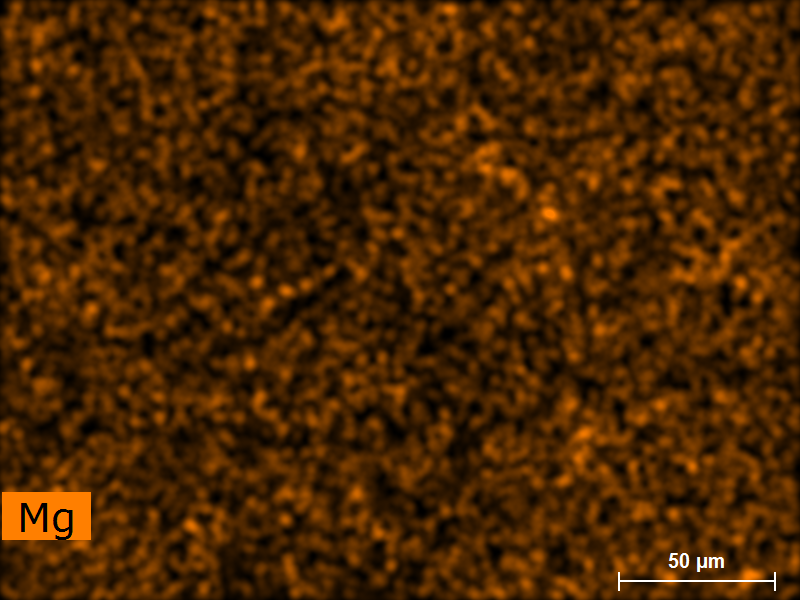
\includegraphics[width=\textwidth]{figs/I/SE_Mg.png}
        \caption{Mg}
        \label{fig:Mg_I}
    \end{subfigure}
    \hfill
    \begin{subfigure}[b]{0.24\textwidth}
        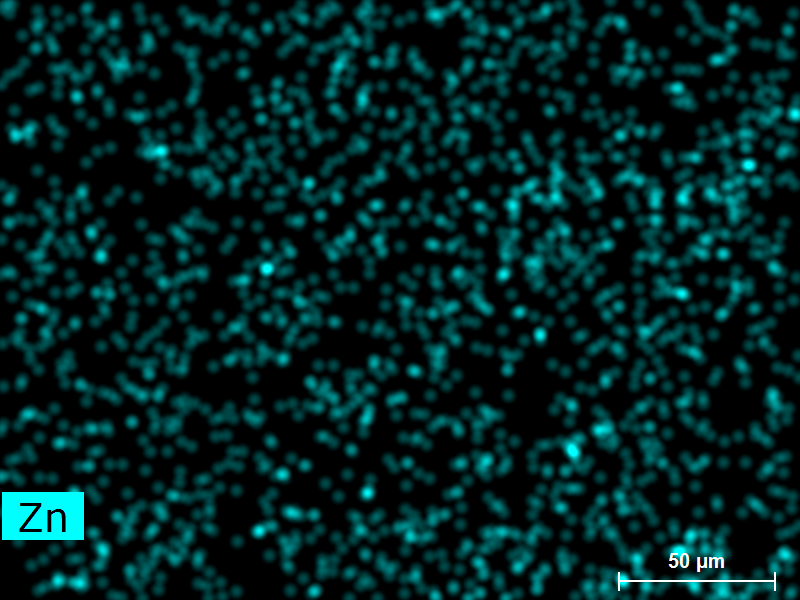
\includegraphics[width=\textwidth]{figs/I/SE_Zn.png}
        \caption{Zn}
        \label{fig:Zn_I}
    \end{subfigure}
    \caption{SEM-EDS elemental maps of mechanically polished specimens.}
    \label{fig:sem_eds_I}
\end{figure}

\begin{figure}[htbp]
   \centering
   \begin{subfigure}[b]{0.24\textwidth}
       
\includegraphics[width=\textwidth]{figs/II/SE_SE.png}
       \caption{SEM}
       \label{fig:sem_II}
   \end{subfigure}
   \hfill
   \begin{subfigure}[b]{0.24\textwidth}
       
\includegraphics[width=\textwidth]{figs/II/SE_Al.png}
       \caption{Al}
       \label{fig:Al_II}
   \end{subfigure}   
   \hfill
   \begin{subfigure}[b]{0.24\textwidth}
       
\includegraphics[width=\textwidth]{figs/II/SE_Fe.png}
       \caption{Fe}
       \label{fig:Fe_II}
   \end{subfigure}
   \hfill
   \begin{subfigure}[b]{0.24\textwidth}
       
\includegraphics[width=\textwidth]{figs/II/SE_Cu.png}
       \caption{Cu}
       \label{fig:Cu_II}
   \end{subfigure}
   \begin{subfigure}[b]{0.24\textwidth}
       
\includegraphics[width=\textwidth]{figs/II/SE_Si.png}
       \caption{Si}
       \label{fig:Si_II}
   \end{subfigure}
   \hfill
   \begin{subfigure}[b]{0.24\textwidth}
       
\includegraphics[width=\textwidth]{figs/II/SE_Mn.png}
       \caption{Mn}
        \label{fig:Mn_II}
    \end{subfigure}
    \hfill
    \begin{subfigure}[b]{0.24\textwidth}
        
\includegraphics[width=\textwidth]{figs/II/SE_Mg.png}
        \caption{Mg}
        \label{fig:Mg_II}
    \end{subfigure}
    \hfill
    \begin{subfigure}[b]{0.24\textwidth}
        
\includegraphics[width=\textwidth]{figs/II/SE_Zn.png}
        \caption{Zn}
        \label{fig:Zn_II}
    \end{subfigure}
    \caption{SEM-EDS elemental maps of chemically pre-treated specimens.}
    \label{fig:sem_eds_II}
\end{figure}

\begin{figure}[htbp]
   \centering
   \begin{subfigure}[b]{0.24\textwidth}
       
\includegraphics[width=\textwidth]{figs/III/SE_SE.png}
       \caption{SEM}
       \label{fig:sem_III}
   \end{subfigure}
   \hfill
   \begin{subfigure}[b]{0.24\textwidth}
       
\includegraphics[width=\textwidth]{figs/III/SE_Al.png}
       \caption{Al}
       \label{fig:Al_III}
   \end{subfigure}   
   \hfill
   \begin{subfigure}[b]{0.24\textwidth}
       
\includegraphics[width=\textwidth]{figs/III/SE_Fe.png}
       \caption{Fe}
       \label{fig:Fe_III}
   \end{subfigure}
   \hfill
   \begin{subfigure}[b]{0.24\textwidth}
       
\includegraphics[width=\textwidth]{figs/III/SE_Cu.png}
       \caption{Cu}
       \label{fig:Cu_III}
   \end{subfigure}
   \begin{subfigure}[b]{0.24\textwidth}
       
\includegraphics[width=\textwidth]{figs/III/SE_Si.png}
       \caption{Si}
       \label{fig:Si_III}
   \end{subfigure}
   \hfill
   \begin{subfigure}[b]{0.24\textwidth}
       
\includegraphics[width=\textwidth]{figs/III/SE_Mn.png}
       \caption{Mn}
        \label{fig:Mn_III}
    \end{subfigure}
    \hfill
    \begin{subfigure}[b]{0.24\textwidth}
        
\includegraphics[width=\textwidth]{figs/III/SE_Mg.png}
        \caption{Mg}
        \label{fig:Mg_III}
    \end{subfigure}
    \hfill
    \begin{subfigure}[b]{0.24\textwidth}
        
\includegraphics[width=\textwidth]{figs/III/SE_Zn.png}
        \caption{Zn}
        \label{fig:Zn_III}
    \end{subfigure}
    \caption{SEM-EDS elemental maps of industrially pre-treated specimens.}
    \label{fig:sem_eds_III}
\end{figure}

The EDS maps of the mechanically polished reference specimens (Figure~\ref{fig:sem_eds_I}) reveal a significant presence of Fe--Mn intermetallic particles, consistent with the \ce{Al15(Fe,Mn)3Si2} and related phases characteristic of AC46000, as well as dispersed Cu- and Si-richparticles. Mg and Zn are distributed diffusely across the matrix with no preferential localisation.

Following chemical pre-treatment (Figure~\ref{fig:sem_eds_II}), the larger Fe--Mn intermetallic particles are largely removed, with only small, scattered residual traces of these elements remaining on the surface. Copper shows partial but limited removal, while silicon particles persist largely unaffected. The Mg and Zn distribution remains comparable to the polished reference, and the aluminium matrix appears intact, with no evidence of significant matrix dissolution.

The industrial pre-treatment (Figure~\ref{fig:sem_eds_III}) produces a markedly more aggressive surface modification. Substantial dissolution of the aluminium matrix is evident, and Fe--Mn and Cu intermetallic particles are effectively removed. However, silicon particles remain prominentlyexposed on the surface, and the diffuse Mg and Zn distribution is largely retained.

From these observations, the industrially pre-treated specimens are expected to provide the most favourable surface conditions for homogeneous LDH nucleation and growth, as the near-complete removal of cathodic Fe--Mn and Cu IMPs eliminates the primary sources of localised micro-galvanic activity that drive heterogeneous LDH precipitation, as discussed in Section~\ref{sec:pitting}. The residual Si particles, being electrochemically inert, are not expected to significantly disrupt LDH growth. From a corrosion standpoint, the reduced density of cathodic IMPs is also anticipated to suppress localised pitting in favour of more uniform matrix dissolution, which is considerably less detrimental to the structural integrity of the alloy. The chemically pre-treated specimens are likewise expected to outperform the polished reference in both LDH growth homogeneity and corrosion resistance, albeit to a lesser degree than the industrial pre-treatment, given the incomplete removal of Fe--Mn and Cu particles.

\section{LDH Synthesis}
\label{sec:results_LDH_synthesis}

To determine which pre-treatment yielded the most favourable conditions forLDH growth, films were synthesised on specimens from all three pre-treatment conditions and characterised by XRD analysis. In addition, LDH growth was assessed on specimens subjected to an anodising procedure prior to synthesis, resulting in a total of four substrate conditions being evaluated. The inclusion of the anodised condition was motivated by prior work on the same alloy, which suggested that anodising promotes LDH nucleation and growth. The XRD patterns are presented in Figure~\ref{fig:xrd_ldh}, and complementary SEM-EDS analysis is shown in Figure~\ref{fig:sem_LDH}.

\begin{figure}[htbp]
    \centering
    
\includegraphics[width=0.95\textwidth]{figs/XRD_LDH.pdf} 
    \caption{XRD patterns of LDH films grown on specimens subjected to the four substrate conditions. Reference patterns for the aluminium matrix and silicon eutectic phases are included for comparison. The inset shows the low-angle region highlighting the (003) and (006) basal reflections characteristic of the ZnAl--LDH phase after baseline subtraction.}
    \label{fig:xrd_ldh}
\end{figure}

\begin{figure}[htbp]
   \centering
   \begin{subfigure}[b]{0.24\textwidth}
       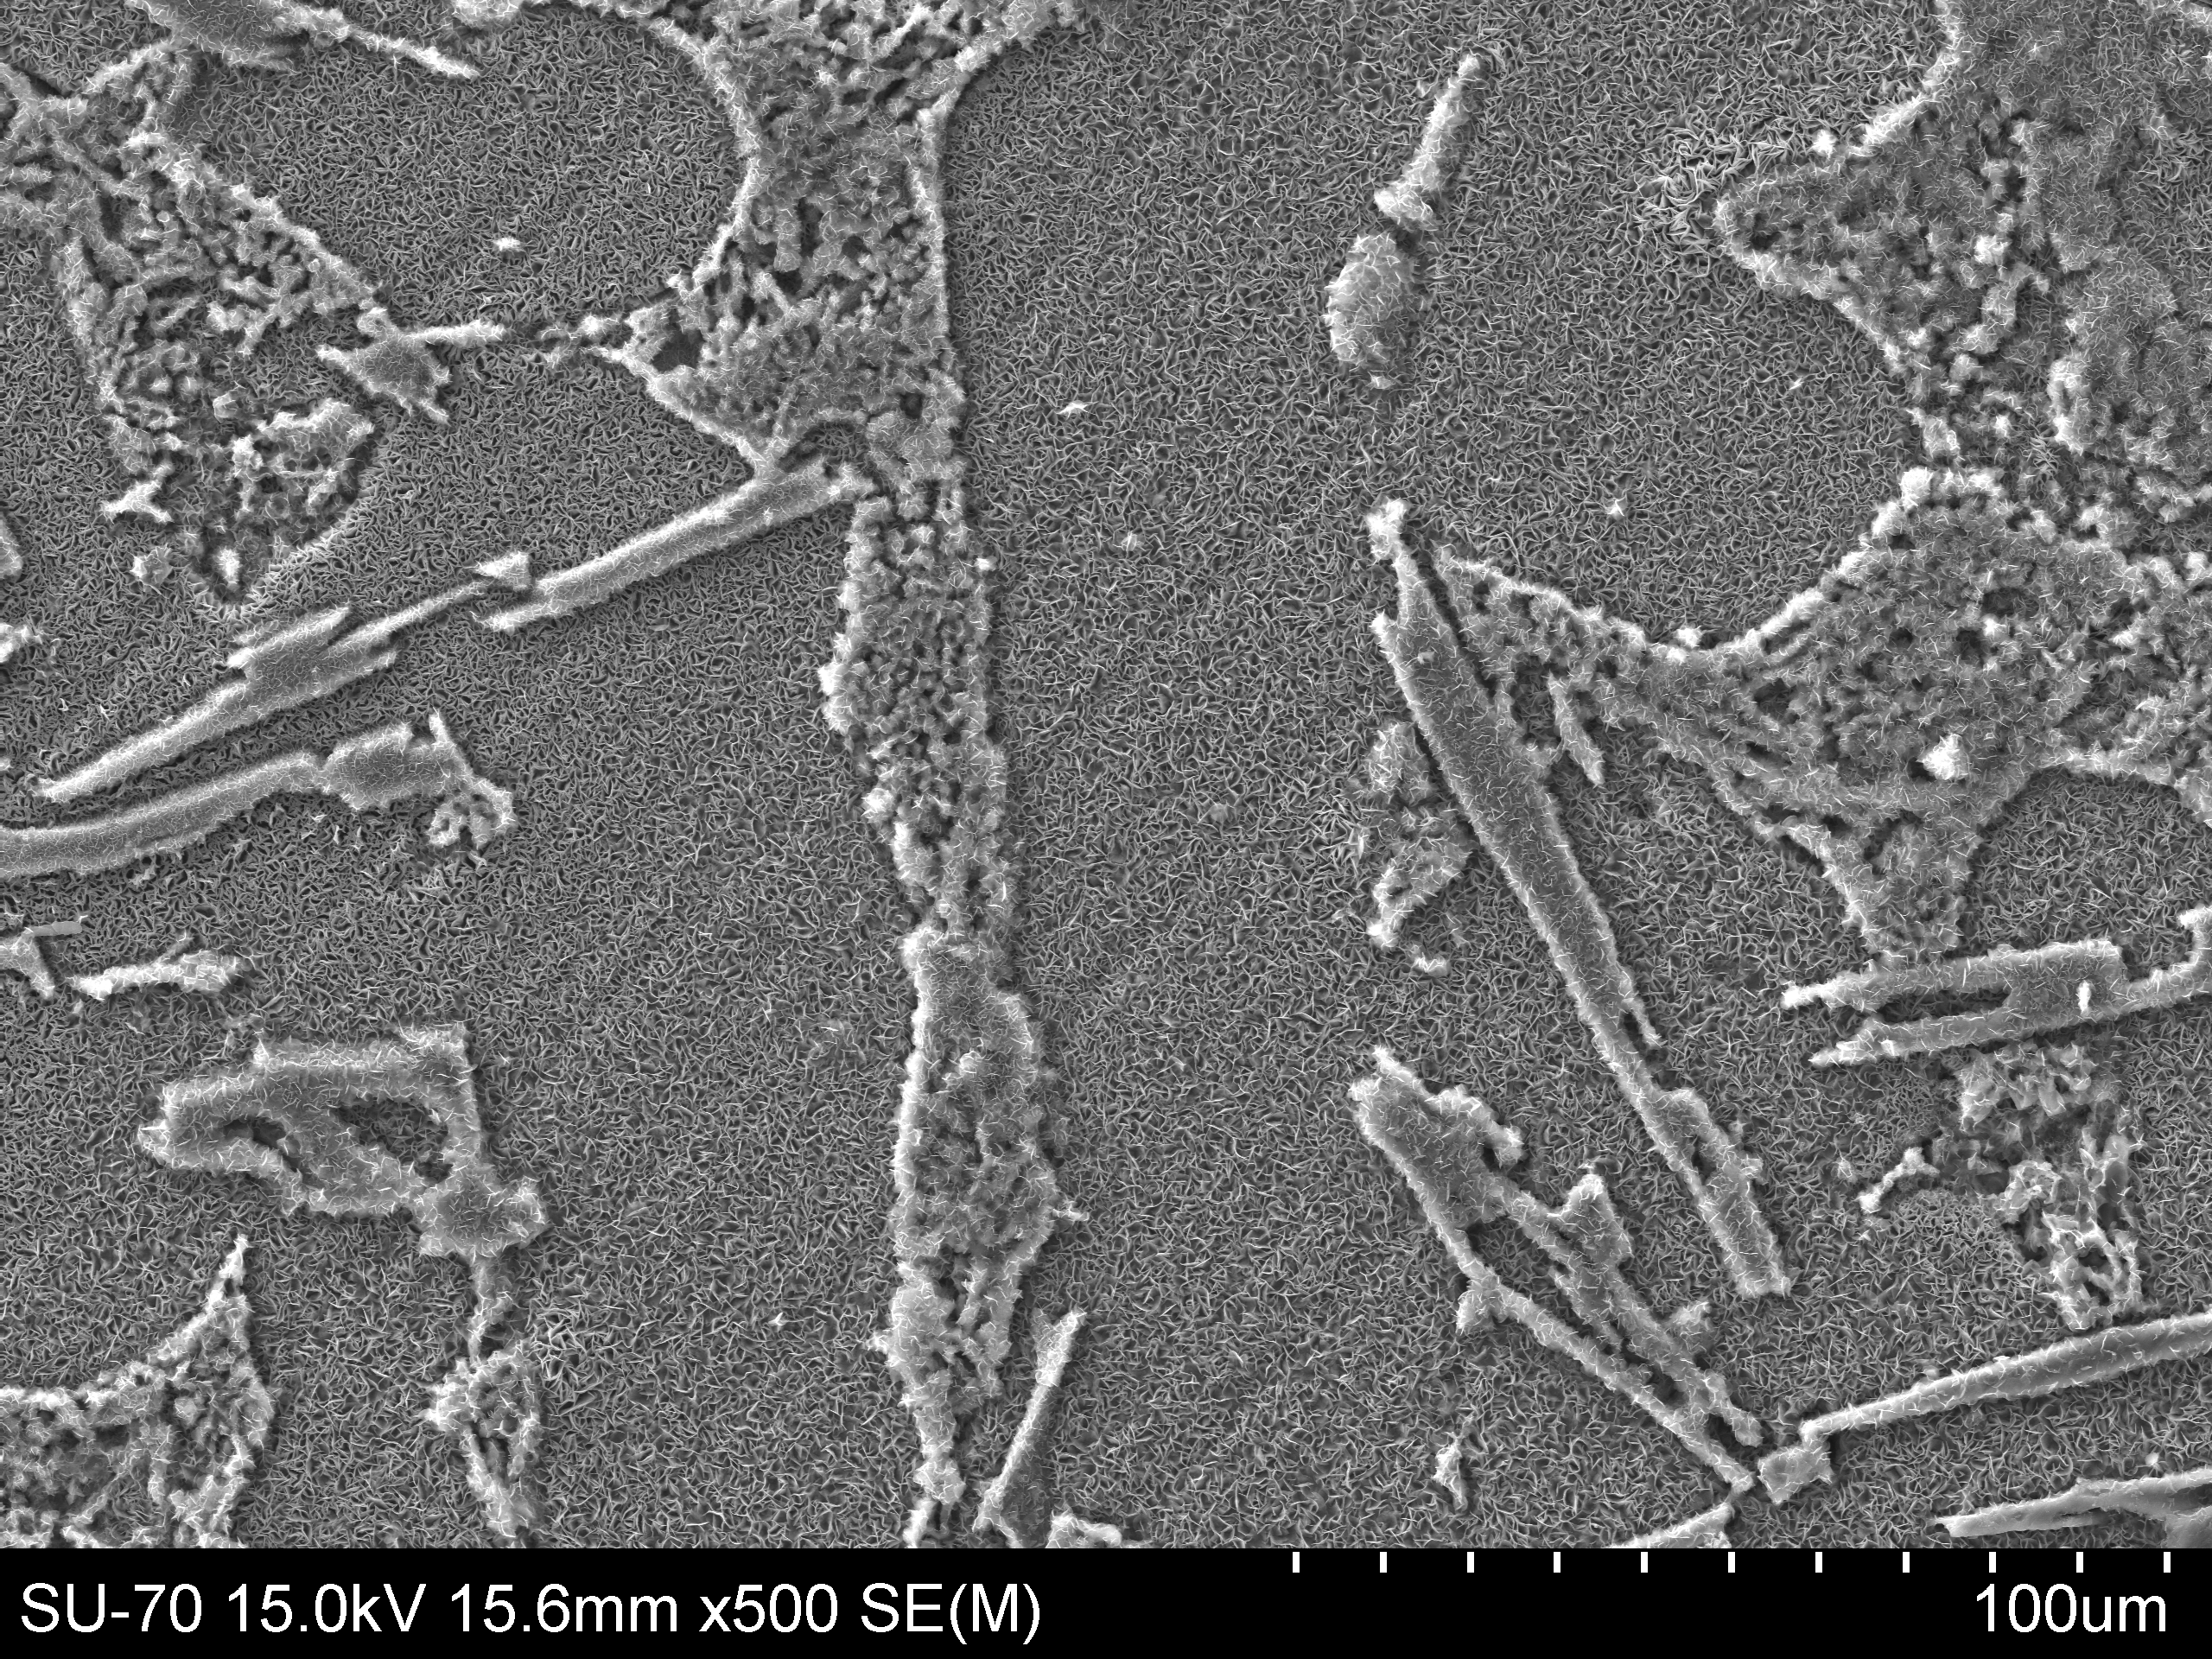
\includegraphics[width=\textwidth]{figs/LDH_SEM/File01.png}
       \caption{}
       \label{fig:sem_LDH_1}
   \end{subfigure}
   \hfill
   \begin{subfigure}[b]{0.24\textwidth}
       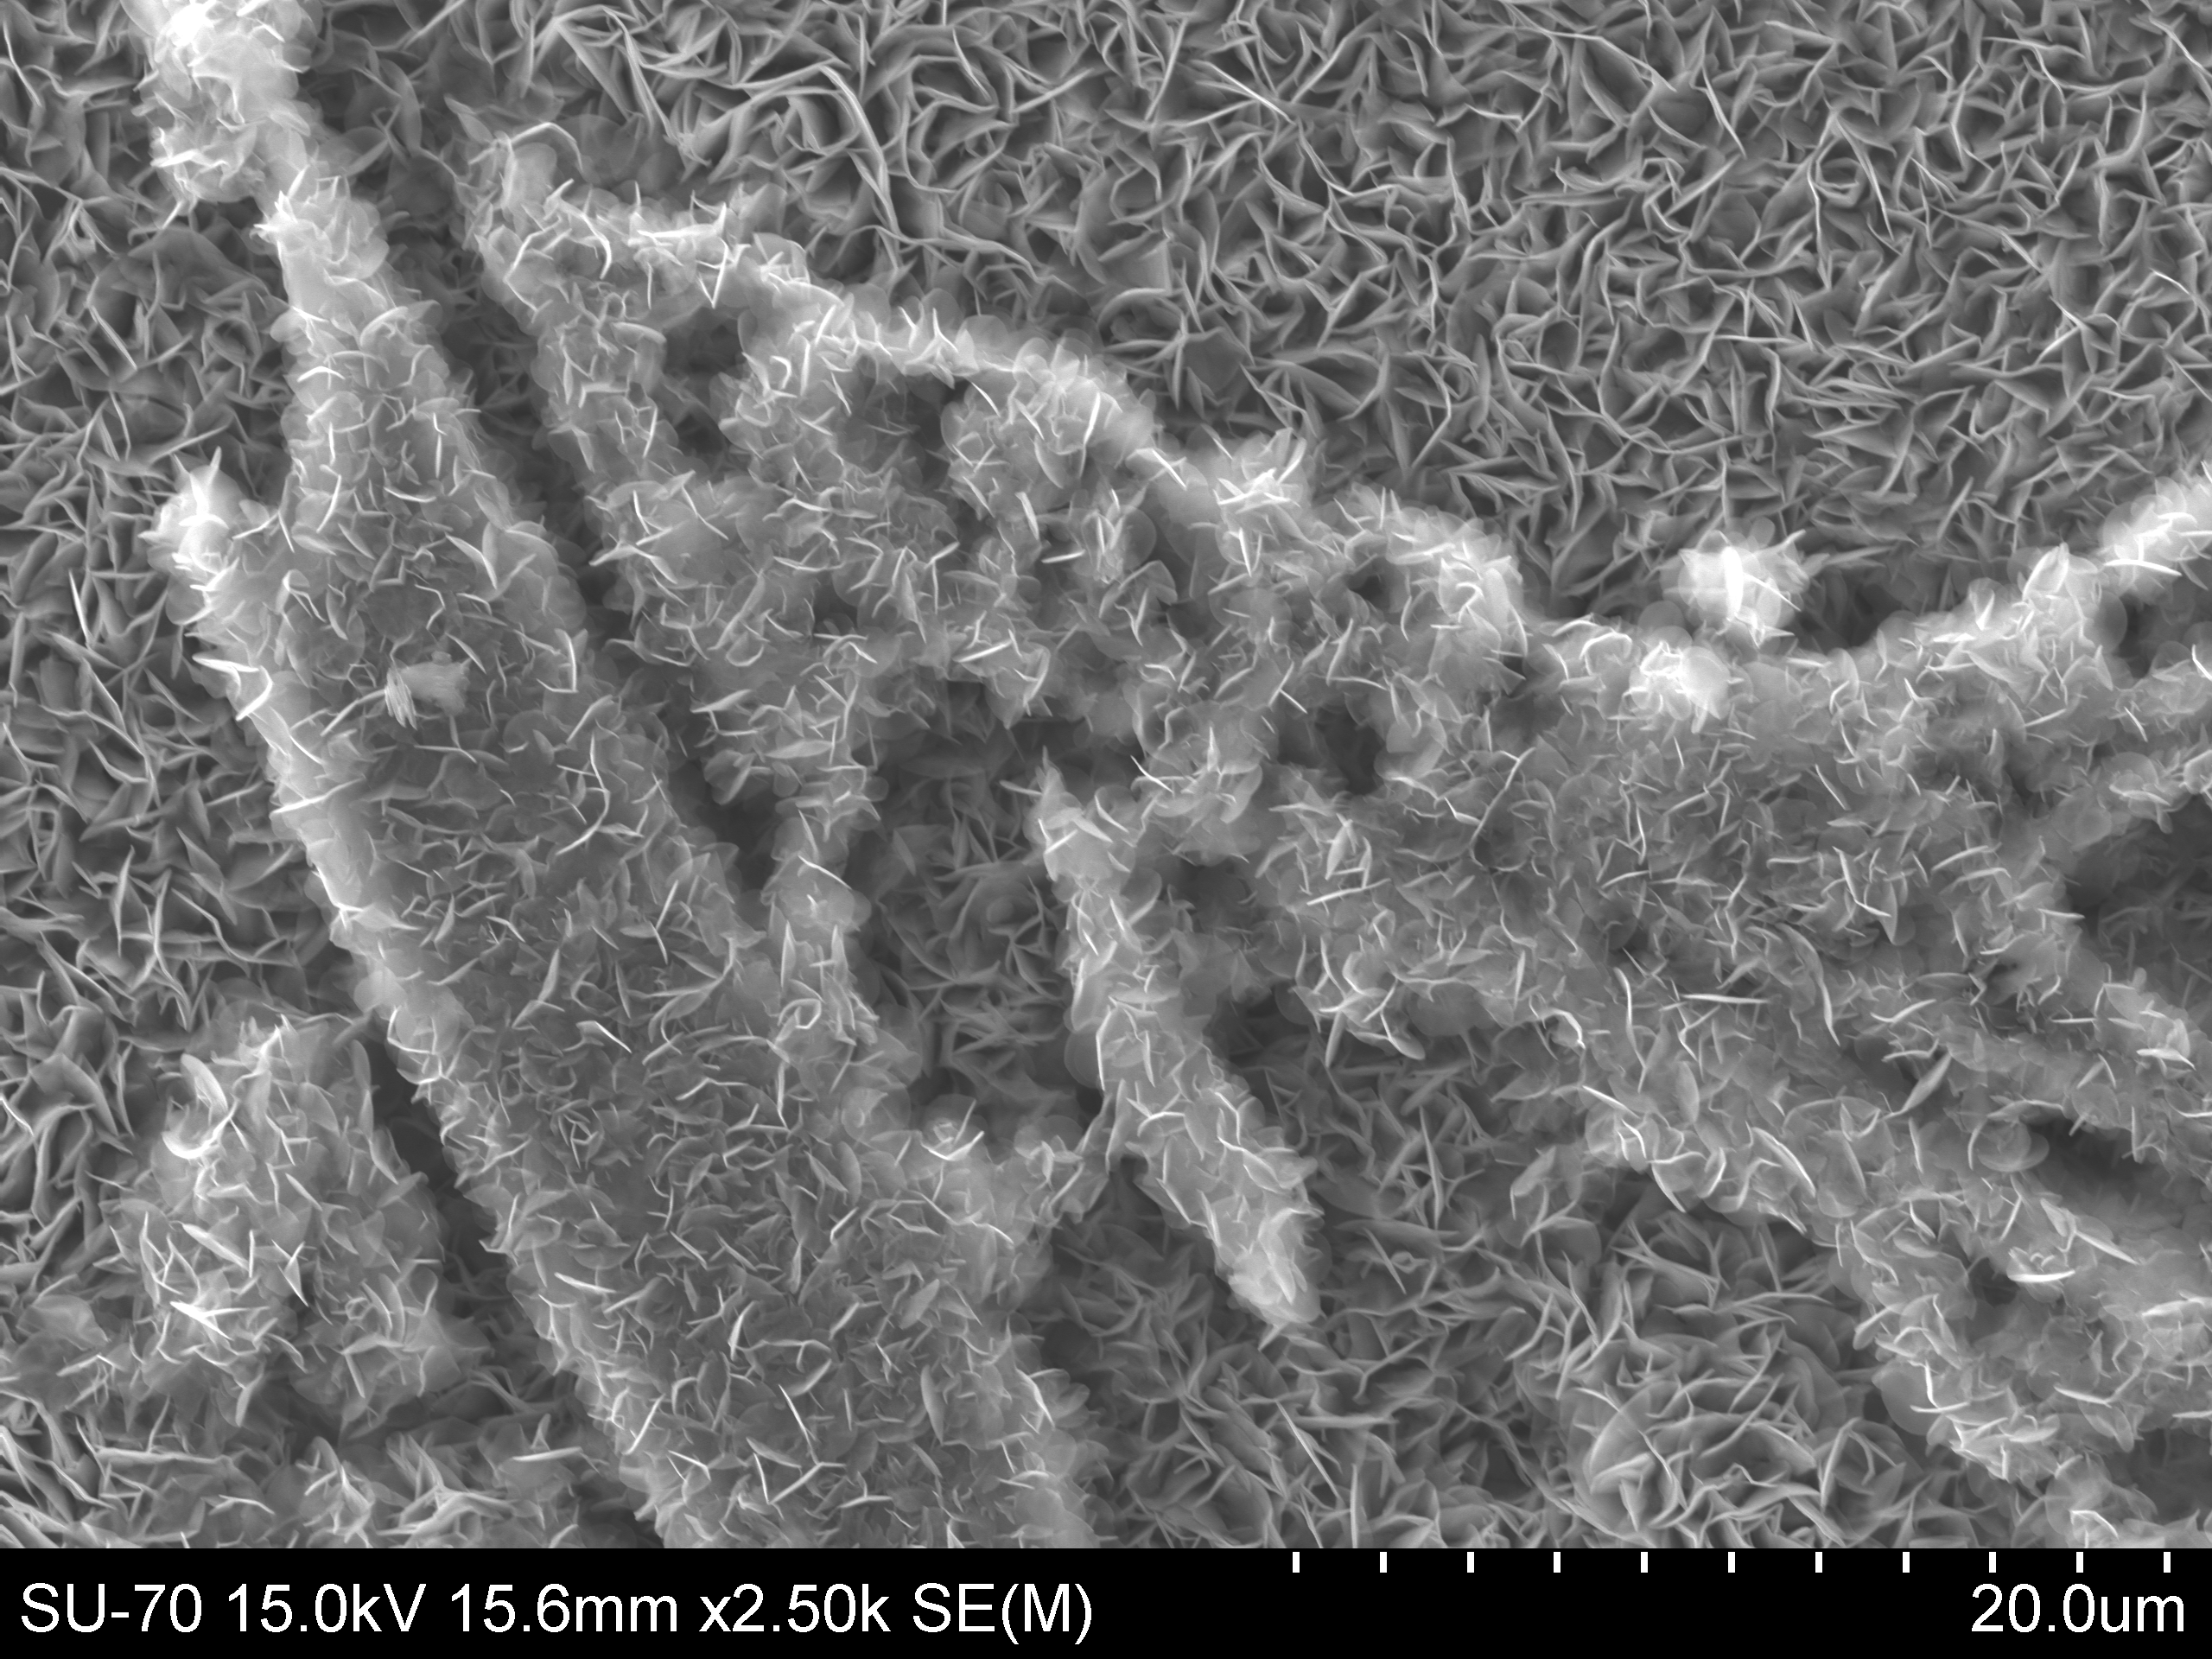
\includegraphics[width=\textwidth]{figs/LDH_SEM/File02.png}
       \caption{}
       \label{fig:sem_LDH_2}
   \end{subfigure}   
   \hfill
   \begin{subfigure}[b]{0.24\textwidth}
       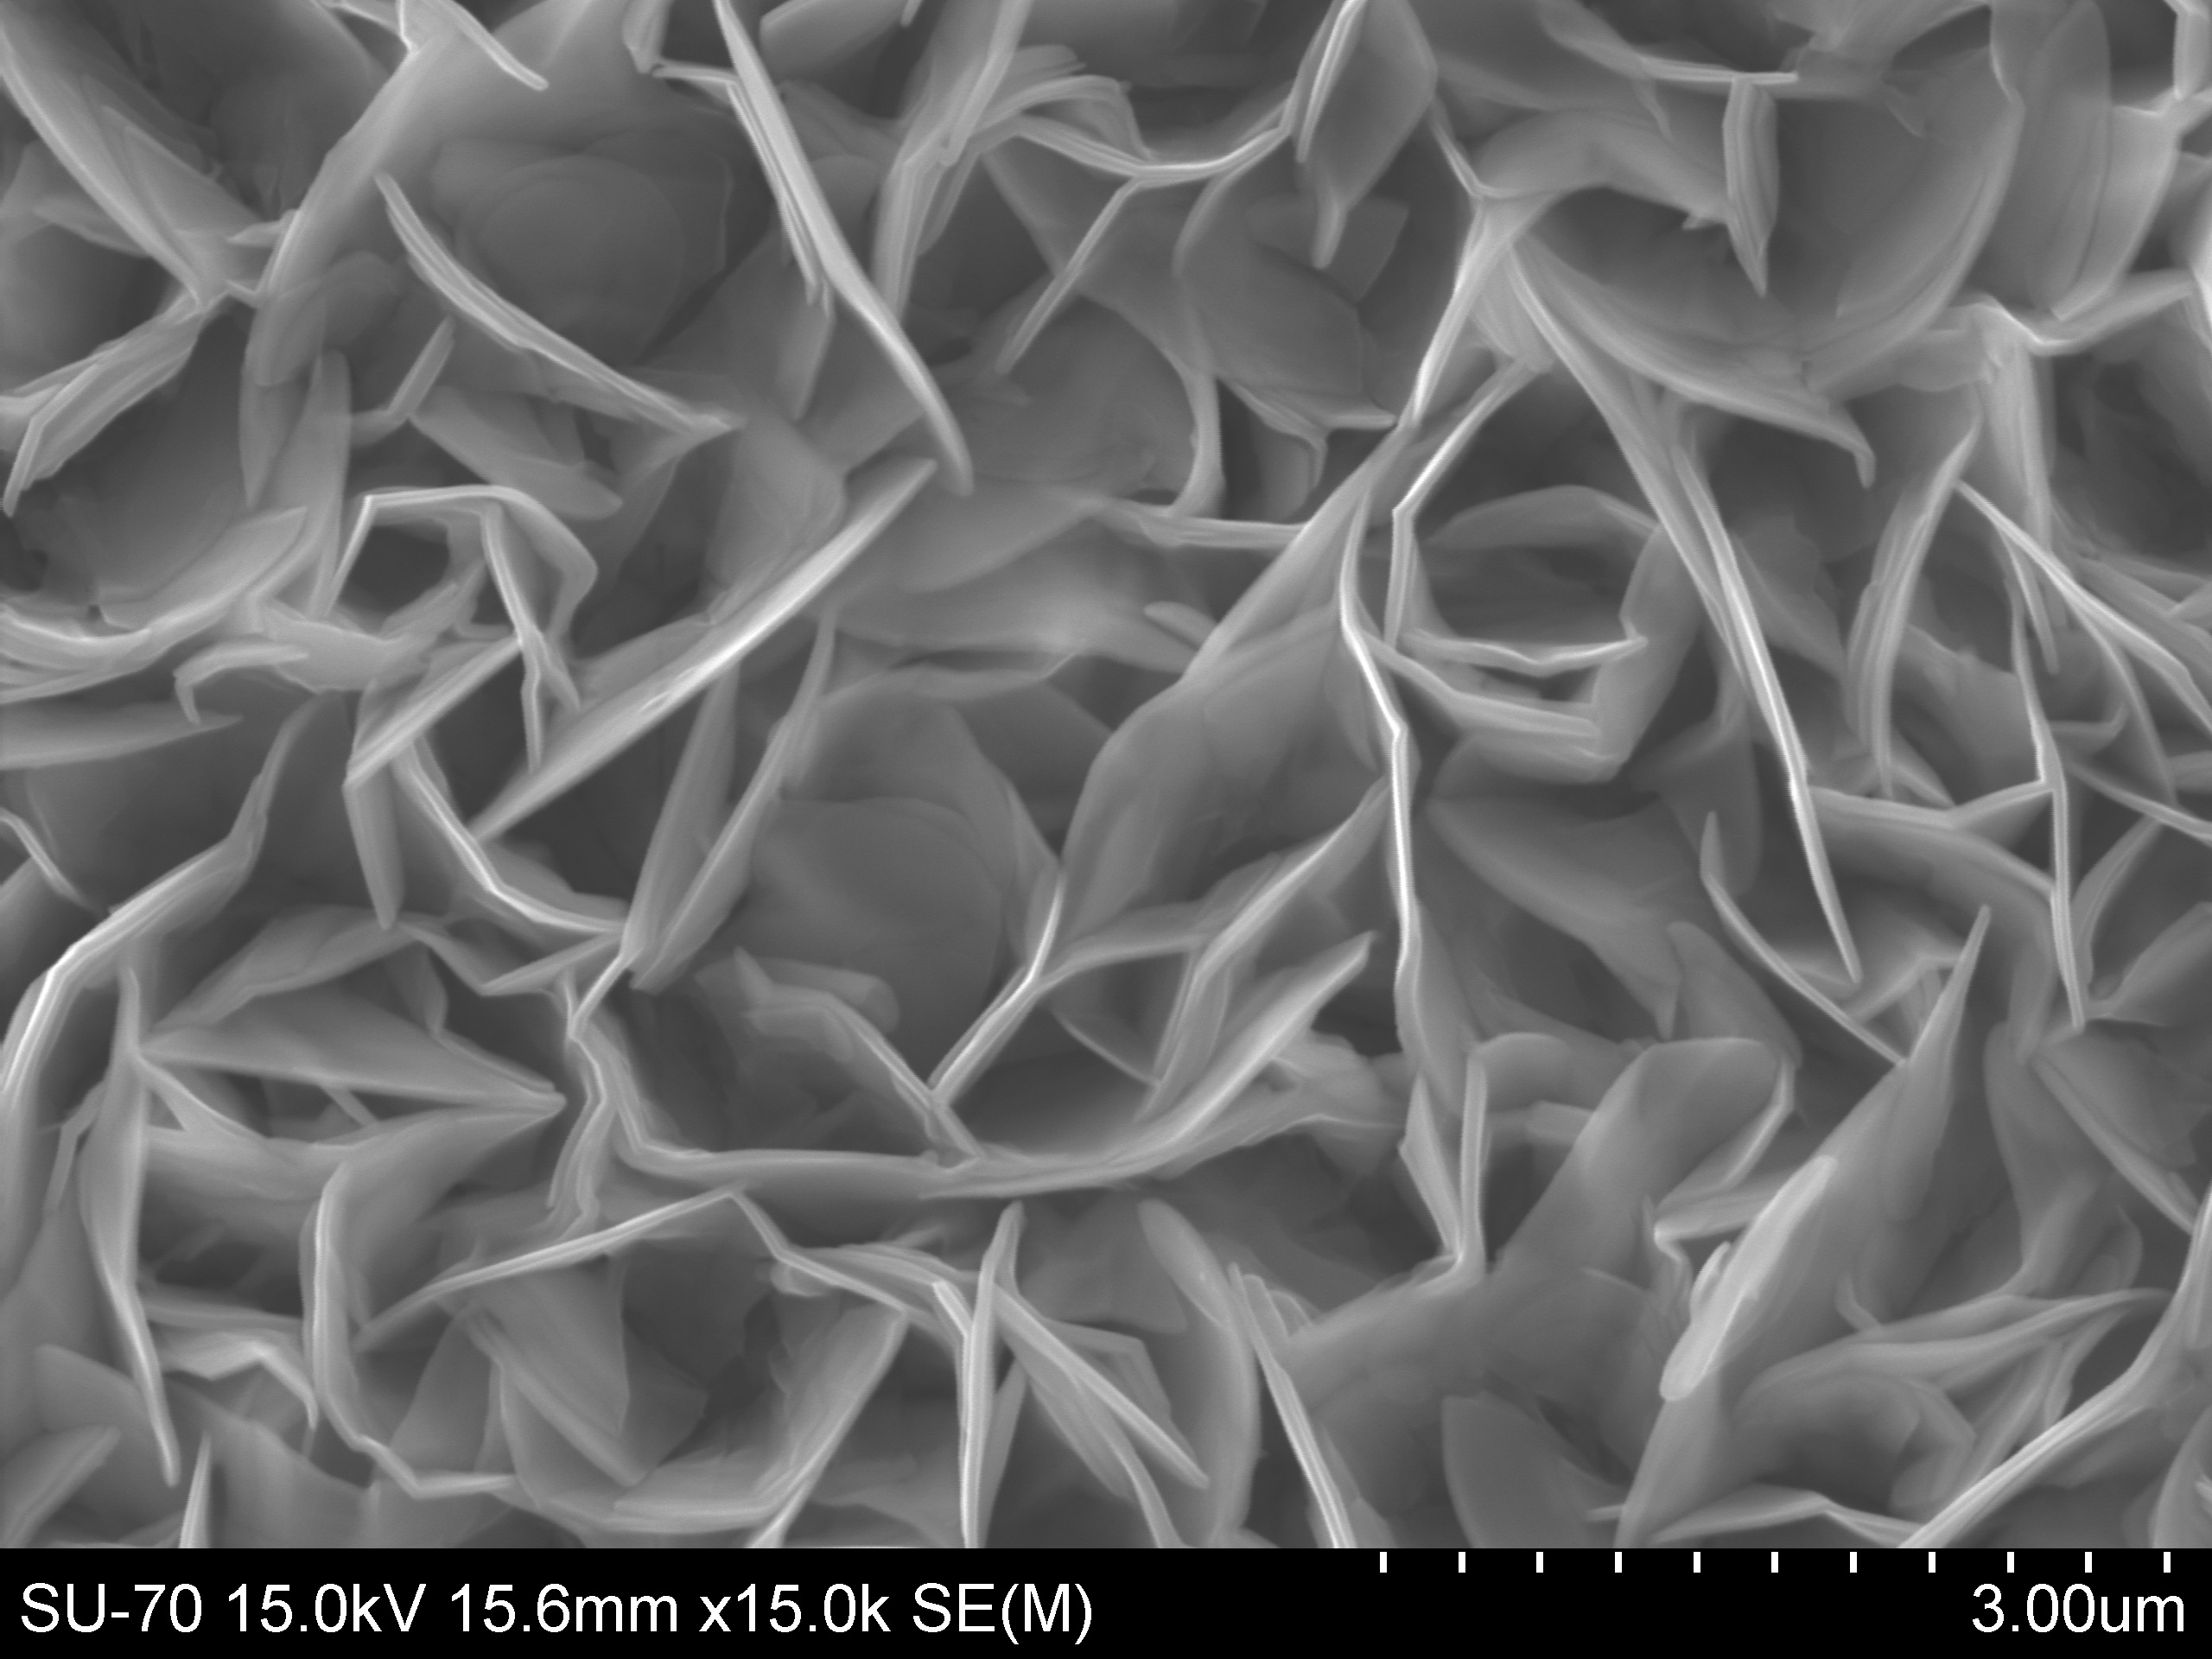
\includegraphics[width=\textwidth]{figs/LDH_SEM/File03.png}
       \caption{}
       \label{fig:sem_LDH_3}
   \end{subfigure}
   \hfill
   \begin{subfigure}[b]{0.24\textwidth}
       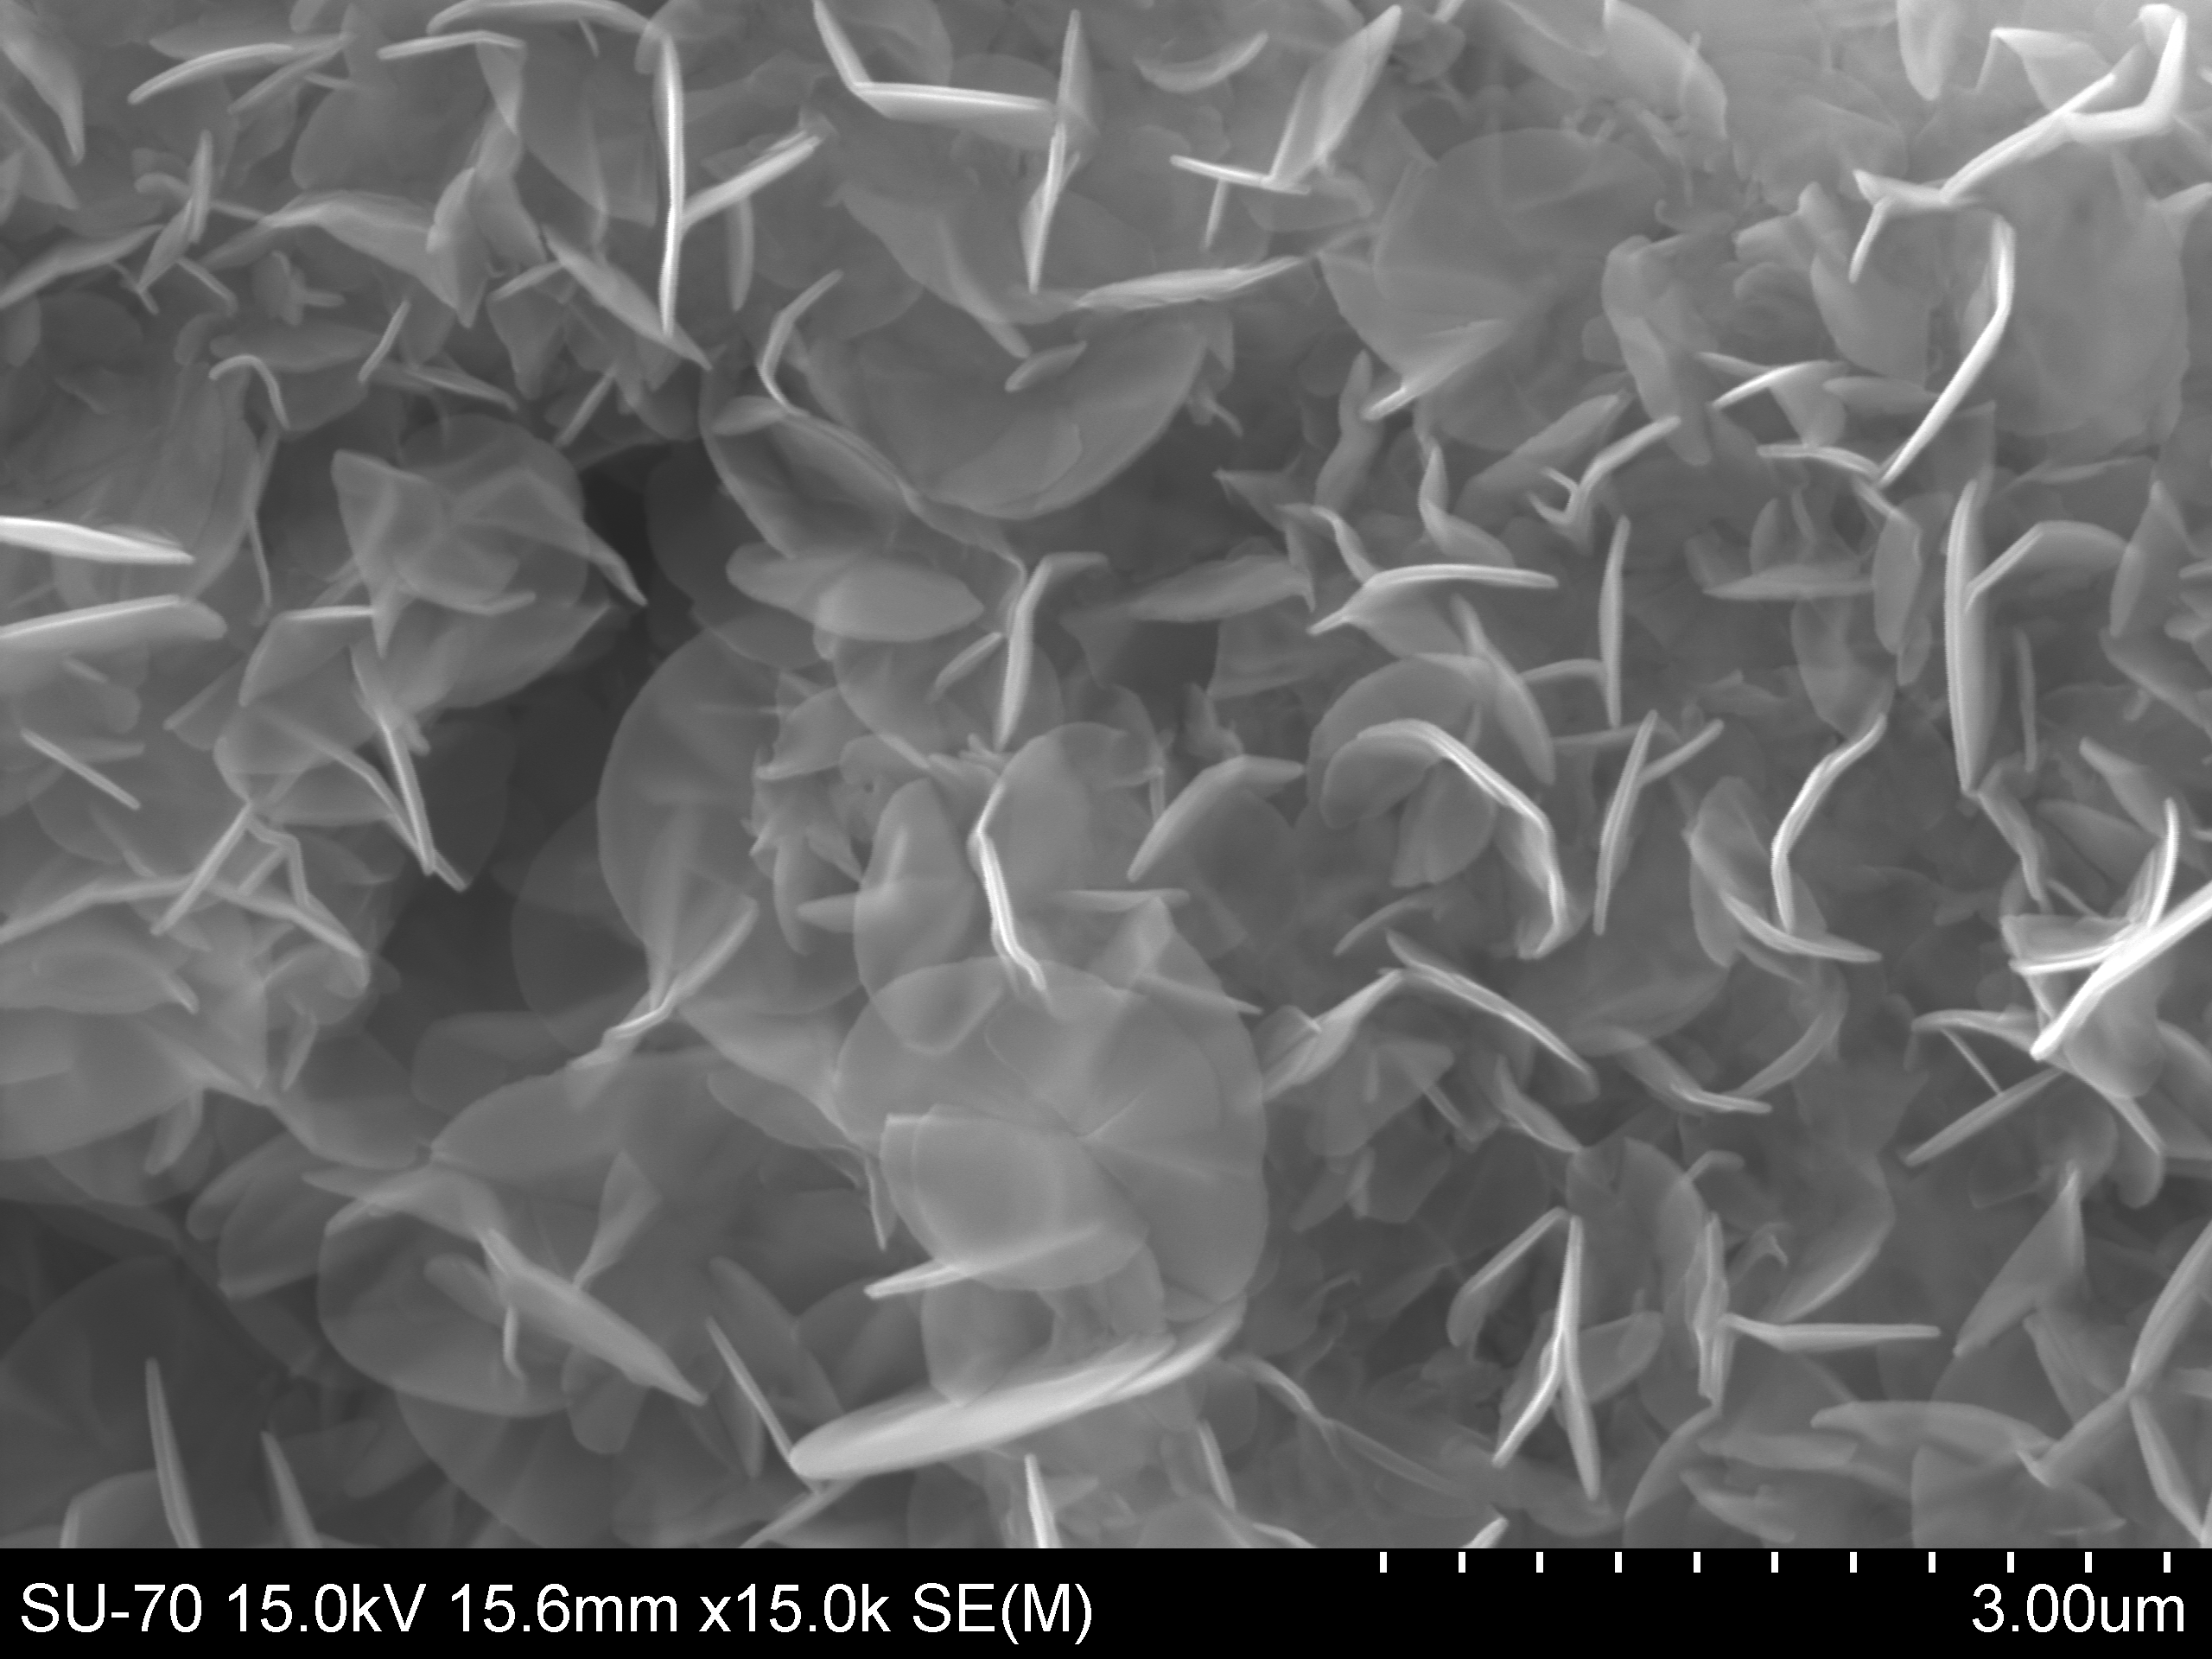
\includegraphics[width=\textwidth]{figs/LDH_SEM/File04.png}
       \caption{}
       \label{fig:sem_LDH_4}
   \end{subfigure}
   \caption{SEM pictures with progressive zoom of LDH films grown on industrially pre-treated specimens. (c) and (d) correspond to zoom-ins on top of aluminium matrix and Si-IMPs respectively.}
   \label{fig:sem_LDH}
\end{figure}

Optical inspection of the LDH films was also conducted to provide a qualitative assessment of film coverage and surface morphology, and is presented in Figure~\ref{fig:optical_LDH}.

\begin{figure}[htbp]
    \centering
    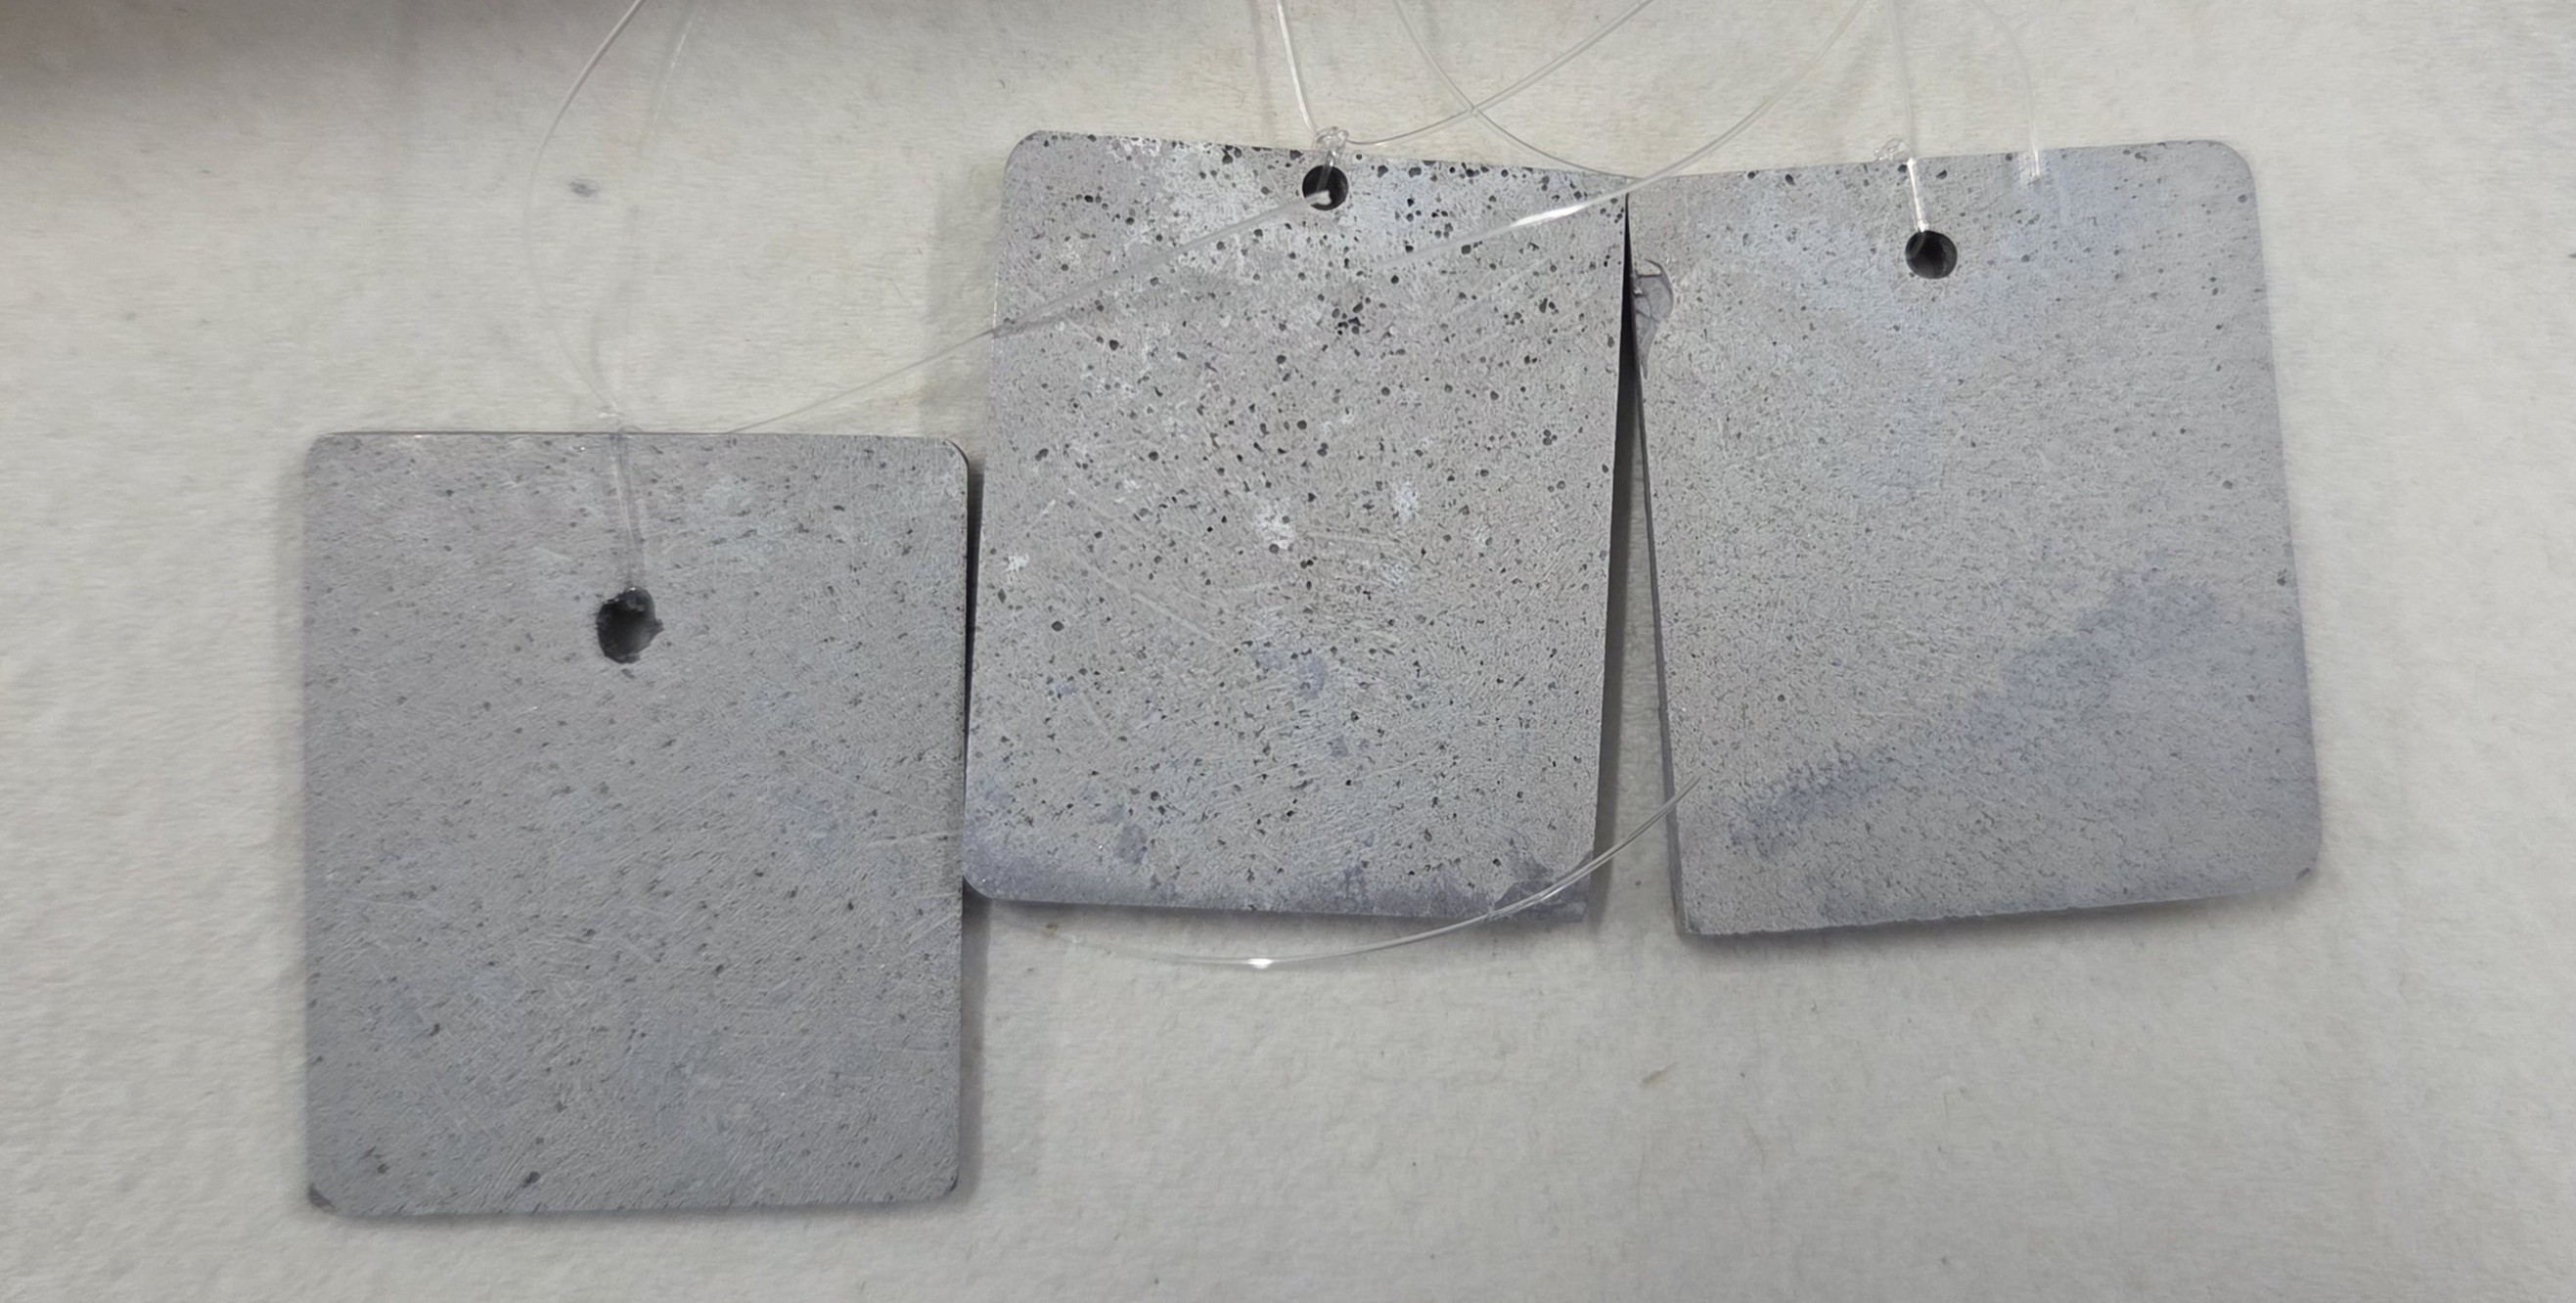
\includegraphics[width=0.5\textwidth]{figs/optical_LDH.jpg}
    \caption{Optical photograph of a representative LDH film grown on an industrially pre-treated specimen.}
    \label{fig:optical_LDH}
\end{figure}

Optical inspection of the LDH films, presented in Figure~\ref{fig:optical_LDH}, reveals generally good surface coverage, albeit not entirely homogeneous across all specimens. The presence of the LDH film is identifiable by its characteristic white appearance. In the central specimen, small dispersed spots of reduced or absent LDH coverage are distributed across the surface, suggesting localised regions where film nucleation was either inhibited or resulted in a film of insufficient density to be visually detectable. The rightmost specimen, by contrast, does not exhibit these scattered spots but instead displays a more pronounced central band of visibly lower LDH density. This spatial inhomogeneity in film coverage is likely associated with the heterogeneous microstructure of the AC46000 die-cast alloy: the casting process gives rise to large, coarse phase regions with distinct local compositions, which respond differently to the alkaline etching and LDH synthesis conditions, resulting in spatially non-uniform \ce{Al^{3+}} availability and consequently uneven LDH nucleation and growth across the surface. 

The XRD patterns confirm successful LDH formation on all four substrate conditions. The reference patterns for the aluminium matrix and silicon eutectic phases are included for comparison. The ZnAl--LDH phase adopts a three-layer rhombohedral stacking sequence (polytype 3R, space group $R\bar{3}m$), which gives rise to the characteristic (003) and (006) basal reflections at approximately $2\theta \approx 10^\circ$ and $2\theta \approx 20^\circ$, respectively \cite{Zhou2017}. The comparable intensities of these reflections across all four substrate conditions indicate that the LDH film density is similar regardless of the pre-treatment applied, and that the anodising procedure confers no measurable advantage in terms of LDH yield or crystallinity. Given that anodising constitutes an additional processing step involving aggressive acid exposure, it was not carried forward in subsequent work.

The basal spacing ($d_{003}$) and interlayer gallery height were determinedfrom the $2\theta$ positions of the (003) reflection using Bragg's law, assuming a brucite layer thickness of \qty{0.477}{\nano\meter} \cite{Zhou2017}. Theresults are summarised in Table~\ref{tab:xrd_pretreatments}.

\begin{table}[htbp]
    \centering
    \small 
    \caption{Structural parameters derived from XRD analysis of LDH films grown on specimens subjected to different pre-treatment conditions.}
    \label{tab:xrd_pretreatments}
    \begin{tabular}{@{} l c c c @{}}
        \toprule
        \makecell[l]{Pre-treatment} & \makecell{$2\theta$ ($^\circ$)} & 
        \makecell{Basal spacing (\AA)} & \makecell{Gallery height  (\AA)} \\
        \midrule
        Chemical etching                & 9.86 & 8.97 & 4.20 \\
        Chemical etching + anodising    & 9.92 & 8.92 & 4.15 \\
        Industrial etching              & 9.94 & 8.90 & 4.13 \\
        Industrial etching + anodising  & 9.92 & 8.92 & 4.15 \\
        \bottomrule
    \end{tabular}
\end{table}

The gallery heights obtained across all conditions range from \qty{4.13}{\angstrom} to \qty{4.20}{\angstrom}, which are consistent with the presence of \ce{NO3^-} as the interlayer anion, given its reported ionic diameter of \qtyrange{3.54}{3.78}{\angstrom} \cite{Zhou2017}. The slight variations in gallery height between conditions are within the expected range of experimental uncertainty and do not indicate any systematic difference in interlayer occupancy attributable to the pre-treatment.

In addition to the XRD analysis, SEM imaging and EDS analysis were conducted on the industrially pre-treated specimens to confirm the presence and spatial distribution of the LDH film. The normalised elemental compositions measured over the aluminium matrix and over silicon eutectic phases are compared in Table~\ref{tab:eds_comparison}.

\begin{table}[htbp]
    \centering
    \small
    \caption{EDS normalised elemental composition of LDH films grown over the aluminium matrix and over silicon eutectic phases on industrially pre-treated specimens.}
    \label{tab:eds_comparison}
    \begin{tabular}{@{} l c c @{}}
        \toprule
        \makecell[l]{Element} & 
        \makecell{Norm. at.\,(\%) (Al matrix)} & 
        \makecell{Norm. at.\,(\%) (Si intermetallic)} \\
        \midrule
        Carbon (C)     & 12.54  & 18.69  \\
        Oxygen (O)     & 45.43  & 41.91  \\
        Aluminium (Al) & 27.47  & 7.19   \\
        Zinc (Zn)      & 8.79   & 8.25   \\
        Silicon (Si)   & 0.52   & 17.28  \\
        Nitrogen (N)   & 5.26   & 6.68   \\
        \midrule
        Total          & 100.00 & 100.00 \\
        \bottomrule
    \end{tabular}
\end{table}

The EDS data reveal the presence of Al, Zn, O, and N across both substrate regions, consistent with the principal constituents of the ZnAl--LDH structure and the intercalated \ce{NO3^-} anions. The most notable difference between the two regions is the substantially elevated Si signal over the intermetallic particles (17.28\,at.\,\%) relative to the matrix (0.52\,at.\,\%), which reflects the underlying Si-rich substrate composition, and the correspondingly reduced Al content (7.19\,at.\,\% versus 27.47\,at.\,\%).

Crucially, the Zn content is nearly identical across both regions --- 8.79\,at.\,\% over the Al matrix and 8.25\,at.\,\% over the Si eutectic phase. Since Zn is absent from the AC46000 alloy and is incorporated exclusively through the synthesis solution, its uniform distribution across both substrate types provides strong and direct evidence that LDH was deposited with comparable density over both the aluminium matrix and the silicon particles.

Further insight is obtained from the Zn:Al atomic ratios. Over the aluminium matrix, the measured Zn:Al ratio is approximately 0.32; however, in this region the Al signal contains contributions from both the LDH film and the underlying aluminium substrate, which inflates the Al denominator and consequently underestimates the true Zn:Al ratio of the LDH film alone. Over the silicon phases, the substrate contributes no Al signal from the Si phase itself, meaning the measured Al derives predominantly from the LDH film. However, the resulting Zn:Al ratio of approximately 1.15, while higher than that measured over the aluminium matrix (0.32), remains below the theoretical Zn:Al ratio of ZnAl--LDH of approximately 2:1 to 3:1 --- corresponding to the $x$ parameter in the general formula, typically in the range $x = 0.25$--$0.33$ \cite{Zhou2017}. This suggests that the Al signal over the Si phase is still partially inflated by a residual contribution from the surrounding aluminium matrix, captured within the lateral spread of the EDS interaction volume at the particle boundaries. Nonetheless, the progressive increase in the Zn:Al ratio from the matrix region to the Si eutectic phase region is consistent with a reduced substrate Al contribution and supports the conclusion that a ZnAl--LDH film of comparable density was deposited over both substrate types. The carbon signal detected in both regions is attributed to the conductive carbon film deposited on the specimens prior to SEM-EDS analysis, a standard sample preparation procedure employed to prevent surface charging during electron beam irradiation.

\section{Inhibitor Intercalation}
\label{sec:results_inhibitor_intercalation}

Using the LDH films produced under the optimal pre-treatment conditions, the three inhibitor systems identified in Section~\ref{sec:results_inhibitor_selection} --- \ce{NaVO3}, MBT, and L-cysteine --- were evaluated for intercalation via anion exchange. XRD analysis was subsequently conducted to verify intercalation, with a shift in the characteristic $2\theta$ reflection angles relative to the nitrate-form LDH serving as evidence of a change in interlayer gallery height and, consequently, of successful replacement of the resident \ce{NO3^-} anions. The XRD patterns before and after intercalation, as well as after immersion in \qty{0.05}{\molar} \ce{NaCl}, are presented in Figure~\ref{fig:xrd_intercalation}.

\begin{figure}[htbp]
    \centering
    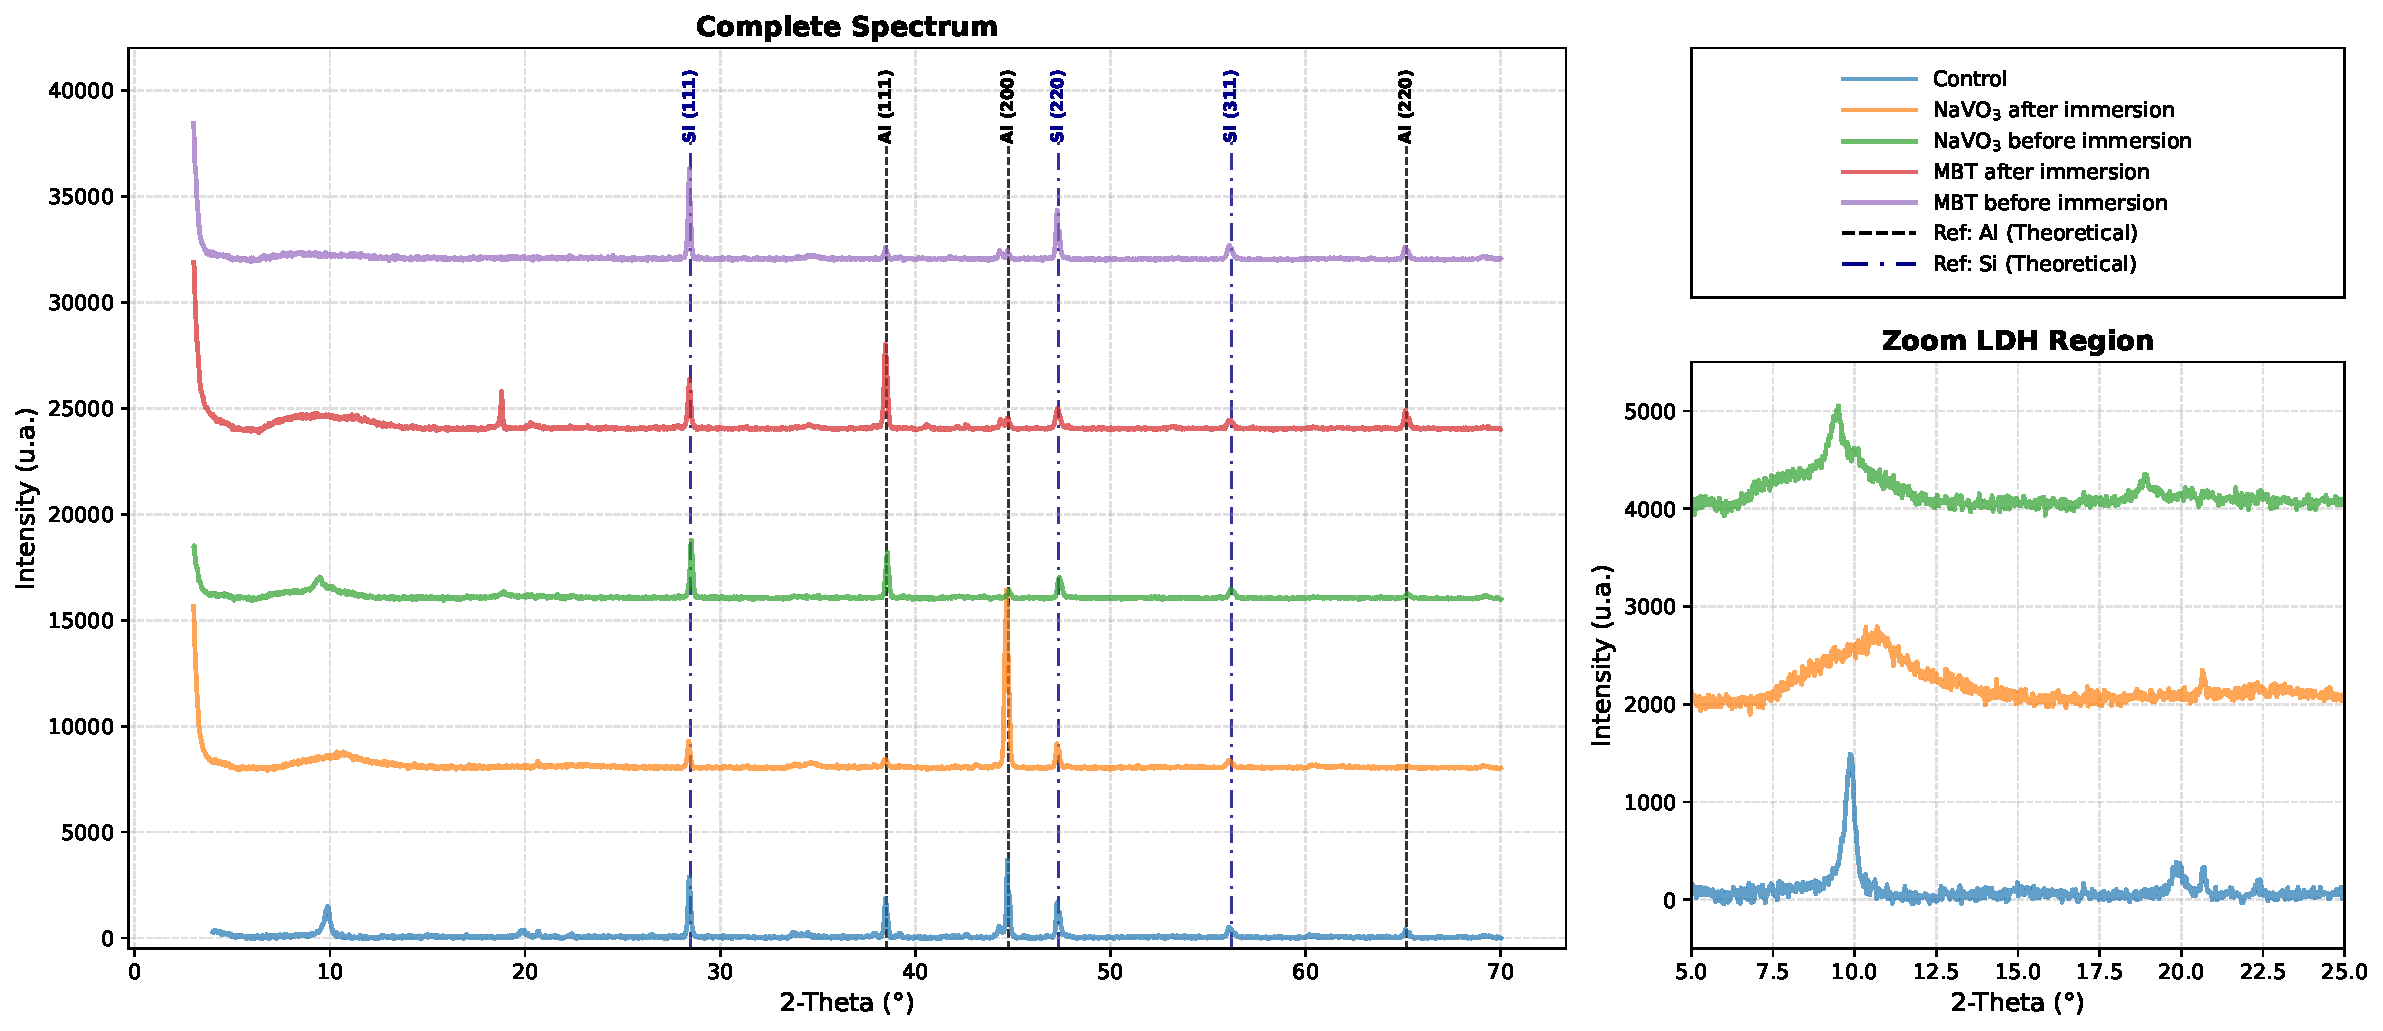
\includegraphics[width=0.95\textwidth]{figs/XRD_intercalation.pdf} 
    \caption{XRD patterns of LDH films in the nitrate form (control), following 
    \ce{NaVO3} intercalation and following MBT intercalation attempt, each 
    presented before and after immersion in \qty{0.05}{\molar} \ce{NaCl}.}
    \label{fig:xrd_intercalation}
\end{figure}

The XRD patterns for the nitrate-form LDH (control), the \ce{NaVO3}-intercalated system, and the MBT intercalation attempt are presented in Figure~\ref{fig:xrd_intercalation}, each shown before and after immersion in \qty{0.05}{\molar} \ce{NaCl}. For \ce{NaVO3}, a clear and systematic shift in the $2\theta$ position of the (003) reflection confirms successful intercalation and subsequent anion exchange during immersion, as discussed in detail below. For MBT, the absence of any discernible diffraction peaks --- both before and after immersion --- confirms the dissolution of the LDH crystalline structure upon exposure to the MBT solution, indicating that intercalation did not occur.

Regarding \ce{NaVO3}, a clear and systematic shift in the $2\theta$ position of the (003) reflection is observed across the three stages. The nitrate-form LDH exhibits a (003) reflection at $2\theta = 9.86^\circ$, corresponding to a basal spacing of \qty{8.97}{\angstrom} and a gallery height of \qty{4.20}{\angstrom}. Following vanadate intercalation, the reflection shifts to $2\theta = 9.51^\circ$, yielding an expanded basal spacing of \qty{9.30}{\angstrom} and a gallery height of \qty{4.53}{\angstrom}, consistent with the accommodation of vanadate species within the interlayer galleries. The observed gallery height expansion relative to the nitrate-form LDH is consistent with the larger effective size of the intercalated vanadate anion, though the precise speciation of the intercalated species --- which may include \ce{VO3^-}, \ce{HVO4^{2-}}, \ce{V2O7^{4-}}, or oligomeric forms depending on local pH and concentration conditions --- was not independently confirmed in this work. After \qty{168}{\hour} of immersion in \ce{NaCl} solution, the reflection shifts further to $2\theta = 10.35^\circ$, corresponding to a reduced basal spacing of \qty{8.55}{\angstrom} and a gallery height of \qty{3.78}{\angstrom}, indicative of the progressive replacement of the larger vanadate anions by the smaller chloride ions (\ce{Cl^-}, ionic radius $\approx$ \qty{1.81}{\angstrom}) through anion exchange during immersion. This confirms that the LDH film actively participates in ion exchange under service conditions, releasing vanadate inhibitor in exchange for the aggressive chloride species present in the electrolyte --- precisely the active protection mechanism for which the system was designed. Alongside the $2\theta$ shift, a progressive broadening and attenuation of the (003) reflection is observed across the three stages, indicating a transition from a well-crystallised LDH structure towards a more amorphous phase. This structural degradation is attributed to two concurrent processes: the partial disruption of the interlayer ordering associated with repeated anion exchange events, and the gradual chemical attack of the LDH film by the corrosive environment itself --- including the locally acidic conditions generated by pit formation and matrix dissolution, as well as the direct interaction of chloride ions with the hydroxide layers --- which progressively undermines the long-range crystalline order of the film during immersion.

In the case of MBT and L-cysteine, however, no diffraction peaks were observed in the XRD spectra following the intercalation attempt, indicating dissolution of the LDH crystalline structure rather than intercalation. The structural degradation is attributed to the thiol group (\ce{-SH}) present in both molecules, which exhibits a strong coordination affinity for \ce{Zn^{2+}} ions and enables these species to act as chelating agents, actively extracting zinc from the host layers and forming soluble zinc--thiolate complexes that destabilise and ultimately collapse the crystal lattice. In the case of L-cysteine, this behaviour was additionally confirmed in a parallel study using a different aluminium substrate but an identical LDH synthesis protocol, where dissolution of the LDH structure was consistently reproduced. Although the solution pH was adjusted prior to intercalation in both cases, the local concentration of reactive thiol groups at the LDH surface is not immediately reduced by pH adjustment alone, and their sustained presence is sufficient to initiate zinc leaching and framework dissolution before intercalation can occur. Notwithstanding this, given the superior inhibition performance demonstrated by MBT in the pre-selection study (Section~\ref{sec:results_inhibitor_selection}), it was decided to proceed with its evaluation in the corrosion performance analysis despite the absence of confirmed crystalline intercalation. In this case, any protective effect is more likely attributable to the remnant amorphous oxide and hydroxide film --- composed principally of aluminium and zinc oxides/hydroxides remaining after LDH dissolution --- acting as a passive barrier, potentially in combination with MBT adsorption onto this residual film, rather than to active inhibitor release through an anion exchange mechanism.

\section{Corrosion Performance Analysis}
\label{sec:results_corrosion_performance}

The corrosion performance of the LDH-based coatings was evaluated in two successive experimental batches. The first batch (LDH-1) comprised specimens subjected to the industrial pre-treatment with a \qty{1}{\hour} LDH growth time, incorporating only \ce{NaVO3} as the interlayer inhibitor, given its status as an established system for aluminium alloy protection. Following analysis of these results, which indicated unsatisfactory corrosion protection performance, the synthesis conditions were revised: the second batch (LDH-2) employed the chemical pre-treatment with an extended LDH growth time of \qty{3}{\hour}, and both \ce{NaVO3} and MBT were evaluated as inhibitor systems. In both cases, corrosion performance was assessed by immersing the specimens in a \qty{0.05}{\molar} \ce{NaCl} solution and conducting EIS measurements at regular intervals over a total immersion period of \qty{168}{\hour}. Potentiodynamic polarisation (PDP) measurements and optical surface inspection were additionally conducted on the LDH-2 specimens to provide complementary information on corrosion kinetics and surface degradation morphology.

\subsection{LDH-1: Industrial Pre-treatment, 1 hour growth}
\label{subsec:ldh1}

\begin{figure}[htbp]
   \centering
   \begin{subfigure}[b]{0.95\textwidth}
       
\includegraphics[width=\textwidth]{figs/bode_1H_LDH_1.pdf}
       \caption{\qty{1}{\hour} immersion.}
       \label{fig:ldh1_1h_bode}
   \end{subfigure}

   \vspace{0.3cm}

   \begin{subfigure}[b]{0.95\textwidth}
       
\includegraphics[width=\textwidth]{figs/bode_168H_LDH_1.pdf}
       \caption{\qty{168}{\hour} immersion.}
       \label{fig:ldh1_168h_bode}
   \end{subfigure}
   \caption{Bode spectra for LDH-1 specimens at \qty{1}{\hour} and 
   \qty{168}{\hour} of immersion in \qty{0.05}{\molar} \ce{NaCl}.}
   \label{fig:ldh1_bode}
\end{figure}

\begin{figure}[htbp]
   \centering
   \begin{subfigure}[b]{0.4\textwidth}
       
\includegraphics[width=\textwidth]{figs/nyquist_1H_LDH_1.pdf}
       \caption{\qty{1}{\hour} immersion.}
       \label{fig:ldh1_1h_nyquist}
   \end{subfigure}
   \begin{subfigure}[b]{0.4\textwidth}
       
\includegraphics[width=\textwidth]{figs/nyquist_168H_LDH_1.pdf}
       \caption{\qty{168}{\hour} immersion.}
       \label{fig:ldh1_168h_nyquist}
   \end{subfigure}   
   \caption{Nyquist spectra for LDH-1 specimens at \qty{1}{\hour} and 
   \qty{168}{\hour} of immersion in \qty{0.05}{\molar} \ce{NaCl}.}
   \label{fig:ldh1_nyquist}
\end{figure}

The Bode and Nyquist spectra for the LDH-1 batch are presented in Figures~\ref{fig:ldh1_bode} and~\ref{fig:ldh1_nyquist}. From the earliest immersion time, the low-frequency impedance modulus of the control specimen exceeds that of all vanadate-intercalated LDH specimens, and this trend is maintained throughout the \qty{168}{\hour} immersion period, indicating that the LDH-coated specimens do not provide a net improvement in barrier performance relative to the uncoated reference under these conditions.

\begin{figure}[htbp]
    \centering
    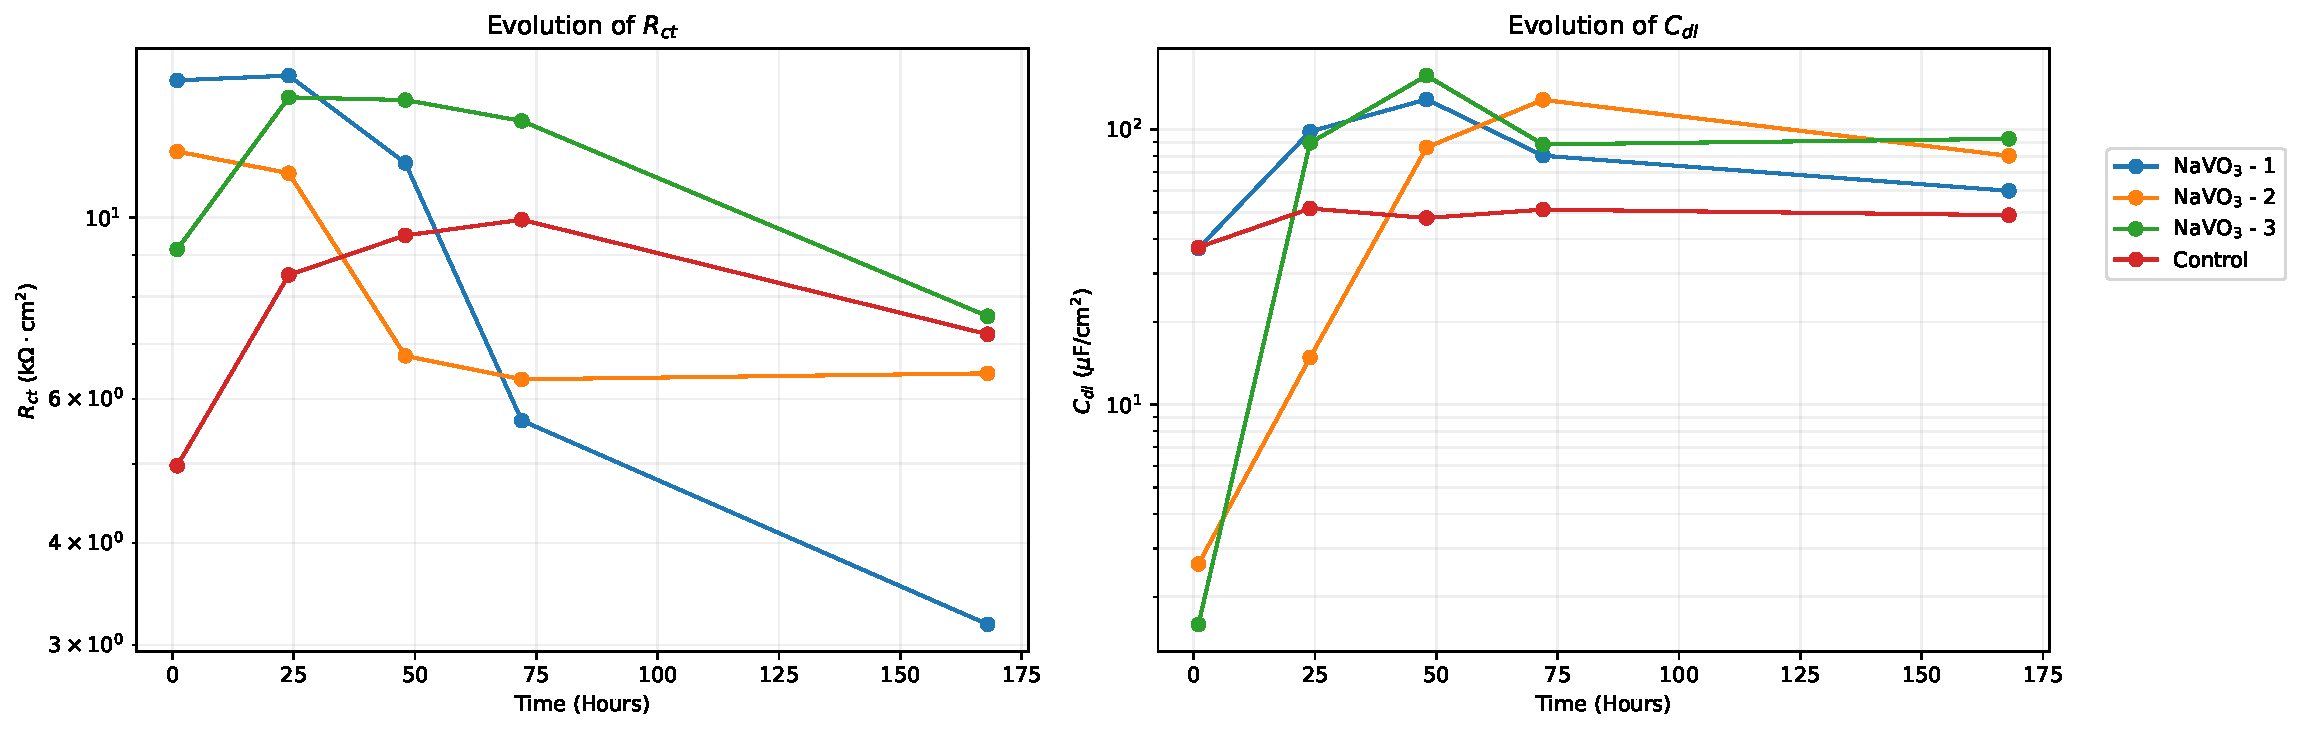
\includegraphics[width=0.95\textwidth]{figs/Rct_Cdl_evolution_LDH1.pdf} 
    \caption{Evolution of $R_{\text{ct}}$ and $C_{\text{dl}}$ as a function of 
    immersion time for LDH-1 specimens in \qty{0.05}{\molar} \ce{NaCl}.}
    \label{fig:Rct_Cdl_evolution_ldh1}
\end{figure}

The evolution of the fitted $R_{\text{ct}}$ and $C_{\text{dl}}$ parameters is shown in Figure~\ref{fig:Rct_Cdl_evolution_ldh1}. Although the vanadate-intercalated specimens initially exhibit higher $R_{\text{ct}}$ values than the control, this advantage is rapidly lost: $R_{\text{ct}}$ decreases steeply with immersion time and is surpassed by the control specimen within the early stages of the experiment, thereafter following a declining trend. The $C_{\text{dl}}$ evolution is similarly unfavourable --- while specimens 2 and 3 display a relatively low initial capacitance, this rises sharply and converges with that of the control and specimen 1, all of which stabilise in the range of 40--100~$\mu$F~cm$^{-2}$, indicative of extensive water uptake and active interfacial corrosion.

\begin{figure}[htbp] %still have to fill in the pictures and do discussion
    \centering
    \begin{subfigure}[b]{0.18\textwidth}
        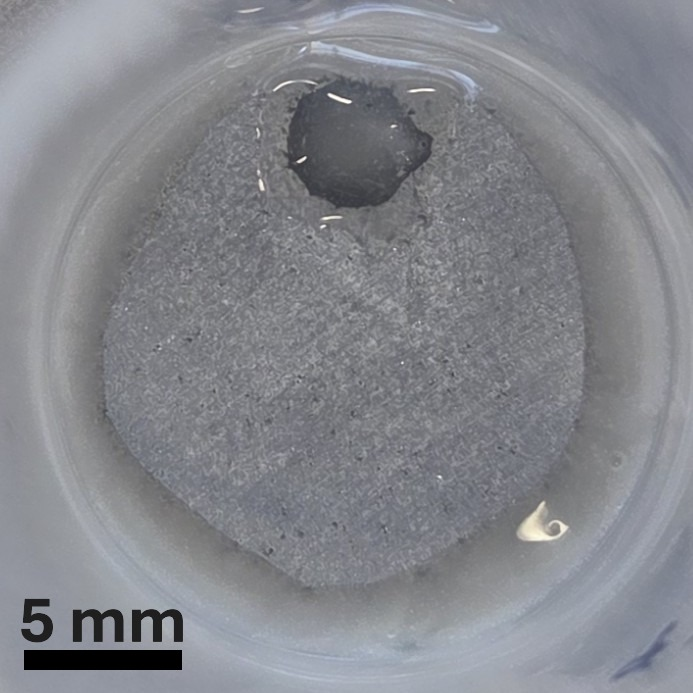
\includegraphics[width=\textwidth]{figs/optical_LDH1/control_before.jpg}
        \caption{Control}
        \label{fig:optical_ldh1_before_control}
    \end{subfigure}
    \begin{subfigure}[b]{0.18\textwidth}
        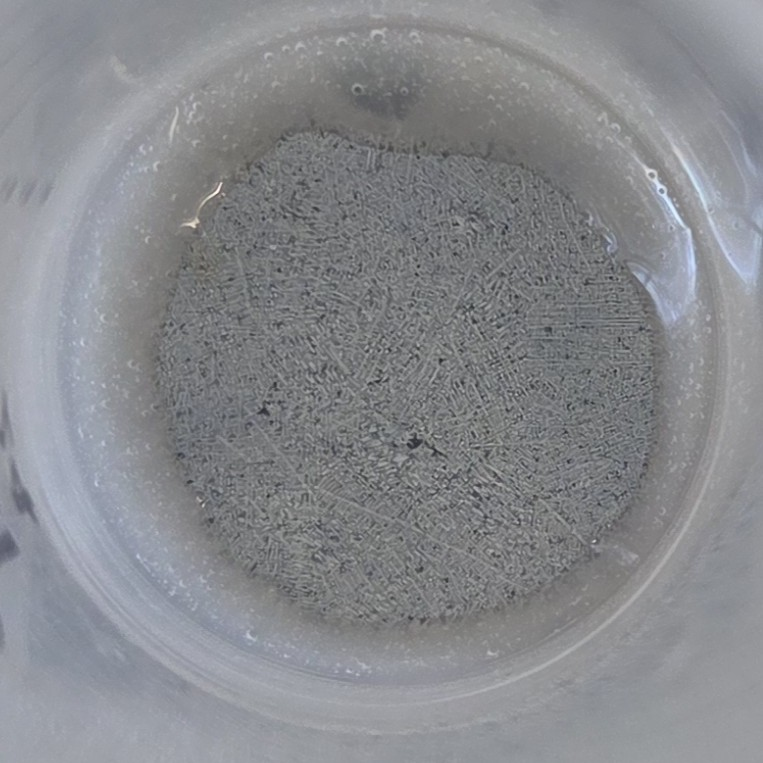
\includegraphics[width=\textwidth]{figs/optical_LDH1/NaVO3_1_before.jpg}
        \caption{\ce{NaVO3} 1}
        \label{fig:optical_ldh1_before_1}
    \end{subfigure}
    \begin{subfigure}[b]{0.18\textwidth}
        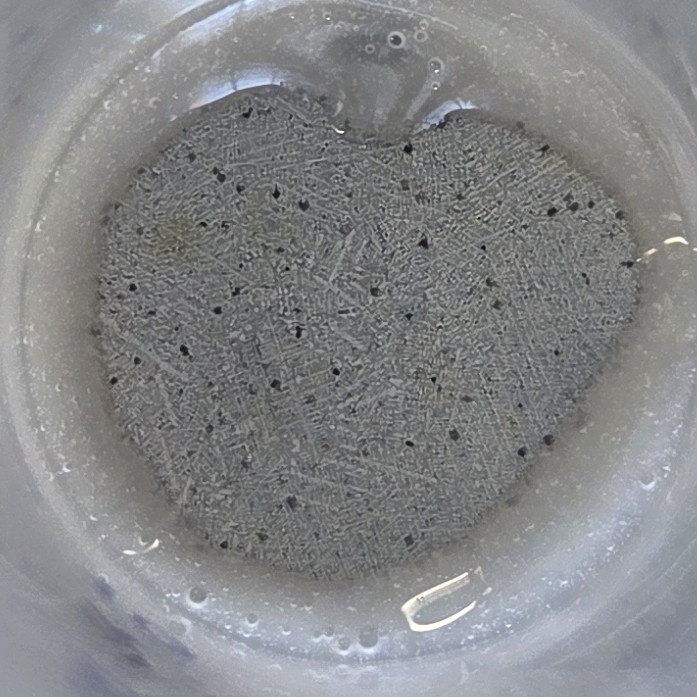
\includegraphics[width=\textwidth]{figs/optical_LDH1/NaVO3_2_before.jpg}
        \caption{\ce{NaVO3} 2}
        \label{fig:optical_ldh1_before_2}
    \end{subfigure}
    \begin{subfigure}[b]{0.18\textwidth}
        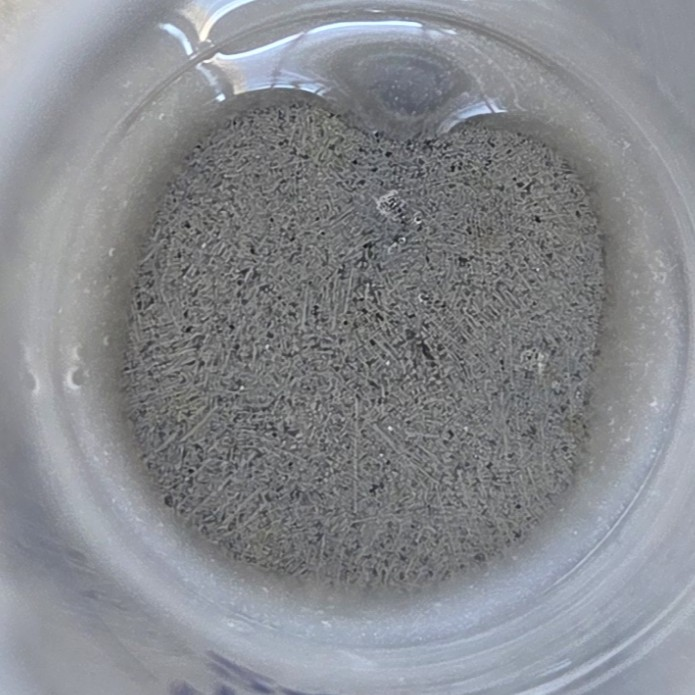
\includegraphics[width=\textwidth]{figs/optical_LDH1/NaVO3_3_before.jpg}
        \caption{\ce{NaVO3} 3}
        \label{fig:optical_ldh1_before_3}
    \end{subfigure}

    \vspace{0.3cm}

    \begin{subfigure}[b]{0.18\textwidth}
        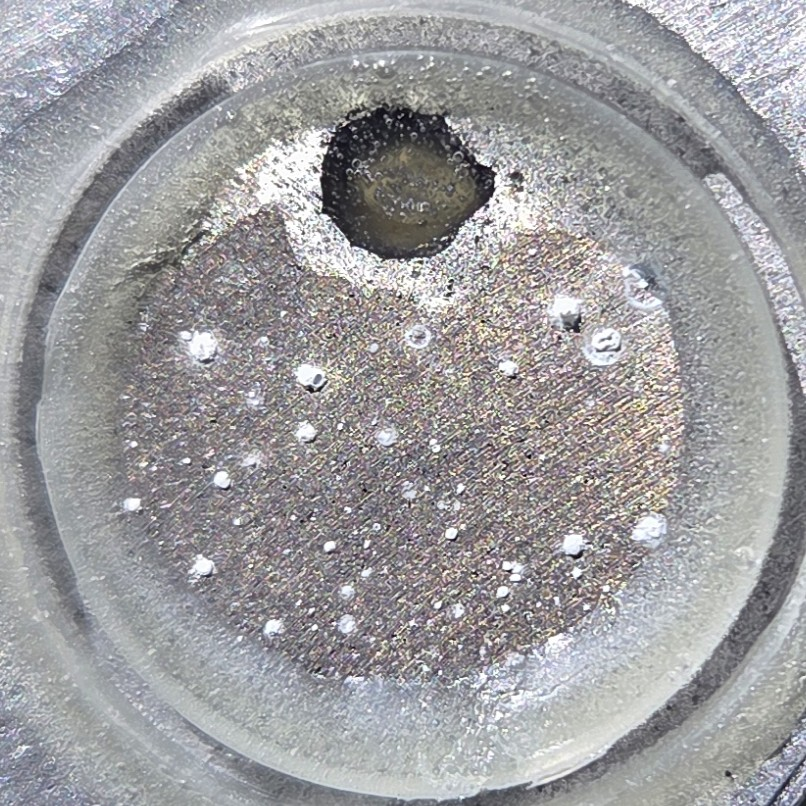
\includegraphics[width=\textwidth]{figs/optical_LDH1/control_after.jpg}
        \caption{Control}
        \label{fig:optical_ldh1_after_control}
    \end{subfigure}
    \begin{subfigure}[b]{0.18\textwidth}
        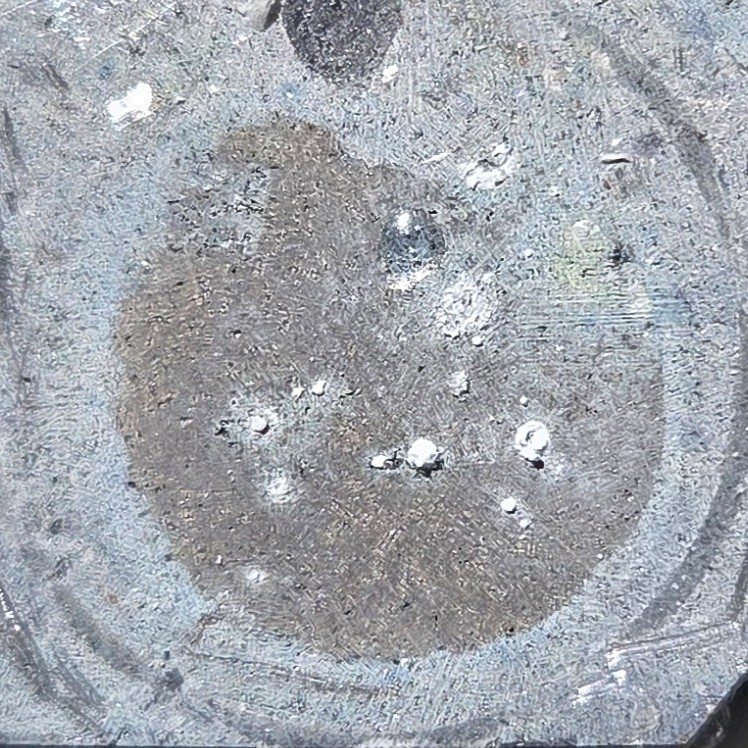
\includegraphics[width=\textwidth]{figs/optical_LDH1/NaVO3_1_after.jpg}
        \caption{\ce{NaVO3} 1}
        \label{fig:optical_ldh1_after_1}
    \end{subfigure}
    \begin{subfigure}[b]{0.18\textwidth}
        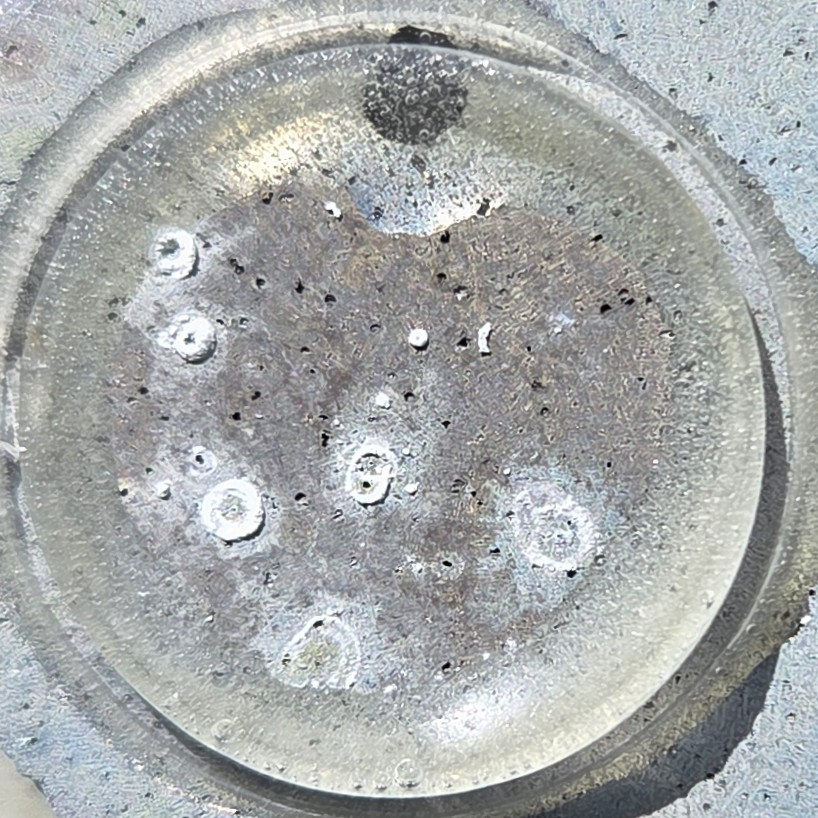
\includegraphics[width=\textwidth]{figs/optical_LDH1/NaVO3_2_after.jpg}
        \caption{\ce{NaVO3} 2}
        \label{fig:optical_ldh1_after_2}
    \end{subfigure}
    \begin{subfigure}[b]{0.18\textwidth}
        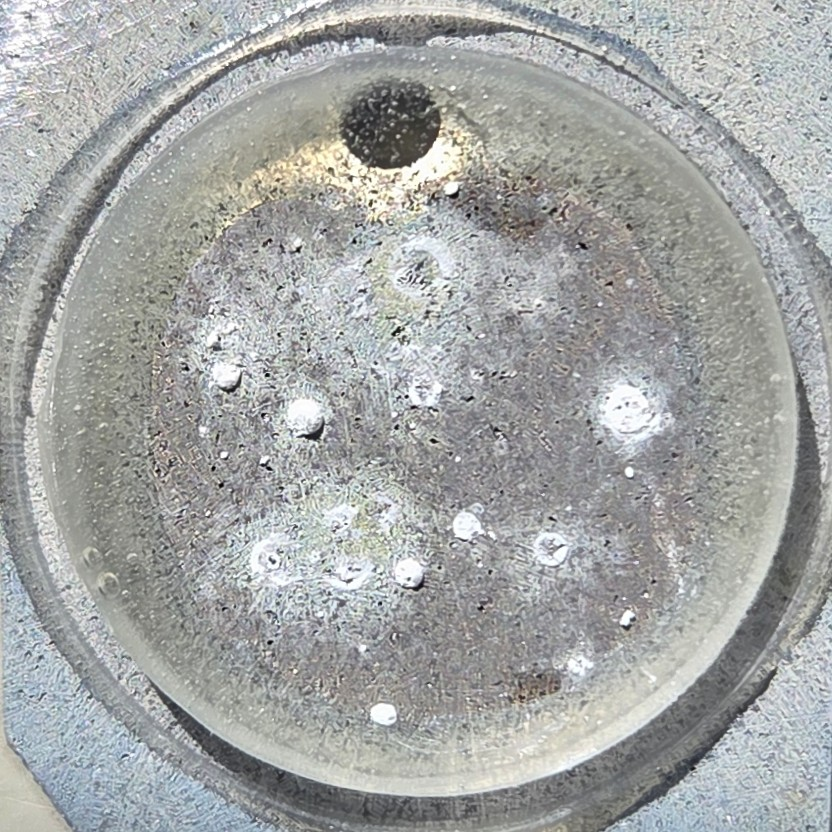
\includegraphics[width=\textwidth]{figs/optical_LDH1/NaVO3_3_after.jpg}
        \caption{\ce{NaVO3} 3}
        \label{fig:optical_ldh1_after_3}
    \end{subfigure}
    \caption{Optical photographs of LDH-1 specimens in \qty{0.05}{\molar} \ce{NaCl}. Top row (a)--(d): prior to immersion. Bottom row (e)--(h): following \qty{168}{\hour} of immersion. (a,e)~Control, (b,f)~\ce{NaVO3}~1, (c,g)~\ce{NaVO3}~2, (d,h)~\ce{NaVO3}~3.}
    \label{fig:optical_ldh1}
\end{figure}

Optical inspection of the LDH-1 specimens prior to and following \qty{168}{\hour} of immersion, presented in Figure~\ref{fig:optical_ldh1}, provides visual confirmation of the electrochemical trends described above. Prior to immersion, all LDH-coated specimens display a uniform surface film with a characteristic yellowish hue, consistent with the successful intercalation of \ce{NaVO3} into the LDH interlayer galleries. Following \qty{168}{\hour} of immersion, all specimens exhibit significant surface degradation. Pitting corrosion is identifiable by localised whitish deposits of aluminium oxide and hydroxide corrosion products. The control specimen displays the greatest number of pits, though these remain relatively small and discrete. In contrast, the three LDH-coated specimens show considerably larger pit dimensions alongside evidence of generalised matrix corrosion, consistent with the more extensive interfacial area exposed by the subsurface intermetallic particles uncovered during LDH synthesis, as discussed above. Nonetheless, there is limited but discernible evidence of vanadate inhibitor activity in specimens 1 and 3, which display small yellowish deposits characteristic of vanadium oxide precipitation at incipient pit sites --- a hallmark of localised \ce{NaVO3} release and repassivation attempt. That these deposits are present but insufficient to prevent macroscopic corrosion further supports the conclusion that the inhibitor loading achievable within the LDH films grown under the industrial pre-treatment conditions was inadequate to suppress the corrosive activity of the newly exposed cathodic intermetallic sites.

This counterintuitive behaviour is attributed to the combined effect of the industrial pre-treatment and LDH synthesis on the alloy surface. The aggressive industrial etching removes the superficial intermetallic particles, eliminating the cathodic sites that would otherwise drive localised micro-galvanic corrosion; the control specimen therefore benefits from a relatively inert surface. The LDH synthesis, however, requires partial dissolution of the aluminium matrix to supply \ce{Al^{3+}} cations, and the more extensive matrix dissolution associated with the industrial pre-treatment not only exposes subsurface intermetallic particles in the immediate vicinity of the surface, but --- given the aggressive nature of the etching --- can penetrate sufficiently deeply into the substrate to access intermetallic particles that were originally buried well below the surface. These newly exposed cathodic sites, whether at or near the surface or at greater depth, initiate localised pitting corrosion.

Once a pit is initiated, the geometry of the cavity itself further exacerbates the corrosion process. Within the confined volume of a pit, mass transport is severely restricted, preventing the local dissolution products from diffusing away and the bulk electrolyte from replenishing the aggressive species. This mass-transport limitation drives the local chemistry towards increasingly aggressive conditions --- lower pH and higher chloride concentration --- promoting autocatalytic and largely uncontrolled dissolution of the aluminium matrix within the pit. Furthermore, the geometric inaccessibility of the pit interior significantly limits the ability of the vanadate inhibitor to reach and passivate the active cathodic sites within the cavity. Unlike surface-exposed intermetallic particles, where inhibitor species released from the LDH film can readily diffuse to and adsorb on the reactive site, the restricted geometry of the pit severely impedes inhibitor transport, rendering the \ce{NaVO3} loading achievable within the LDH films insufficient to suppress cathodic activity at these buried sites. This assessment motivated a revision of the synthesis protocol for the second batch.

\subsection{LDH-2: Chemical Pre-treatment, 3 hour growth}
\label{subsec:ldh2}

Based on the findings of the LDH-1 batch, the pre-treatment was changed to the milder chemical etching, which --- as demonstrated in Section~\ref{sec:results_LDH_synthesis} --- yields comparable LDH growth without the deep matrix dissolution associated with the industrial procedure. The LDH growth time was extended to \qty{3}{\hour} to increase film density and consequently the inhibitor loading within the interlayer galleries. Both \ce{NaVO3} and MBT were evaluated as inhibitor systems, with MBT selected on the basis of its superior performance in the pre-selection study described in Section~\ref{sec:results_inhibitor_selection}.

\begin{figure}[htbp]
   \centering
   \begin{subfigure}[b]{0.95\textwidth}
       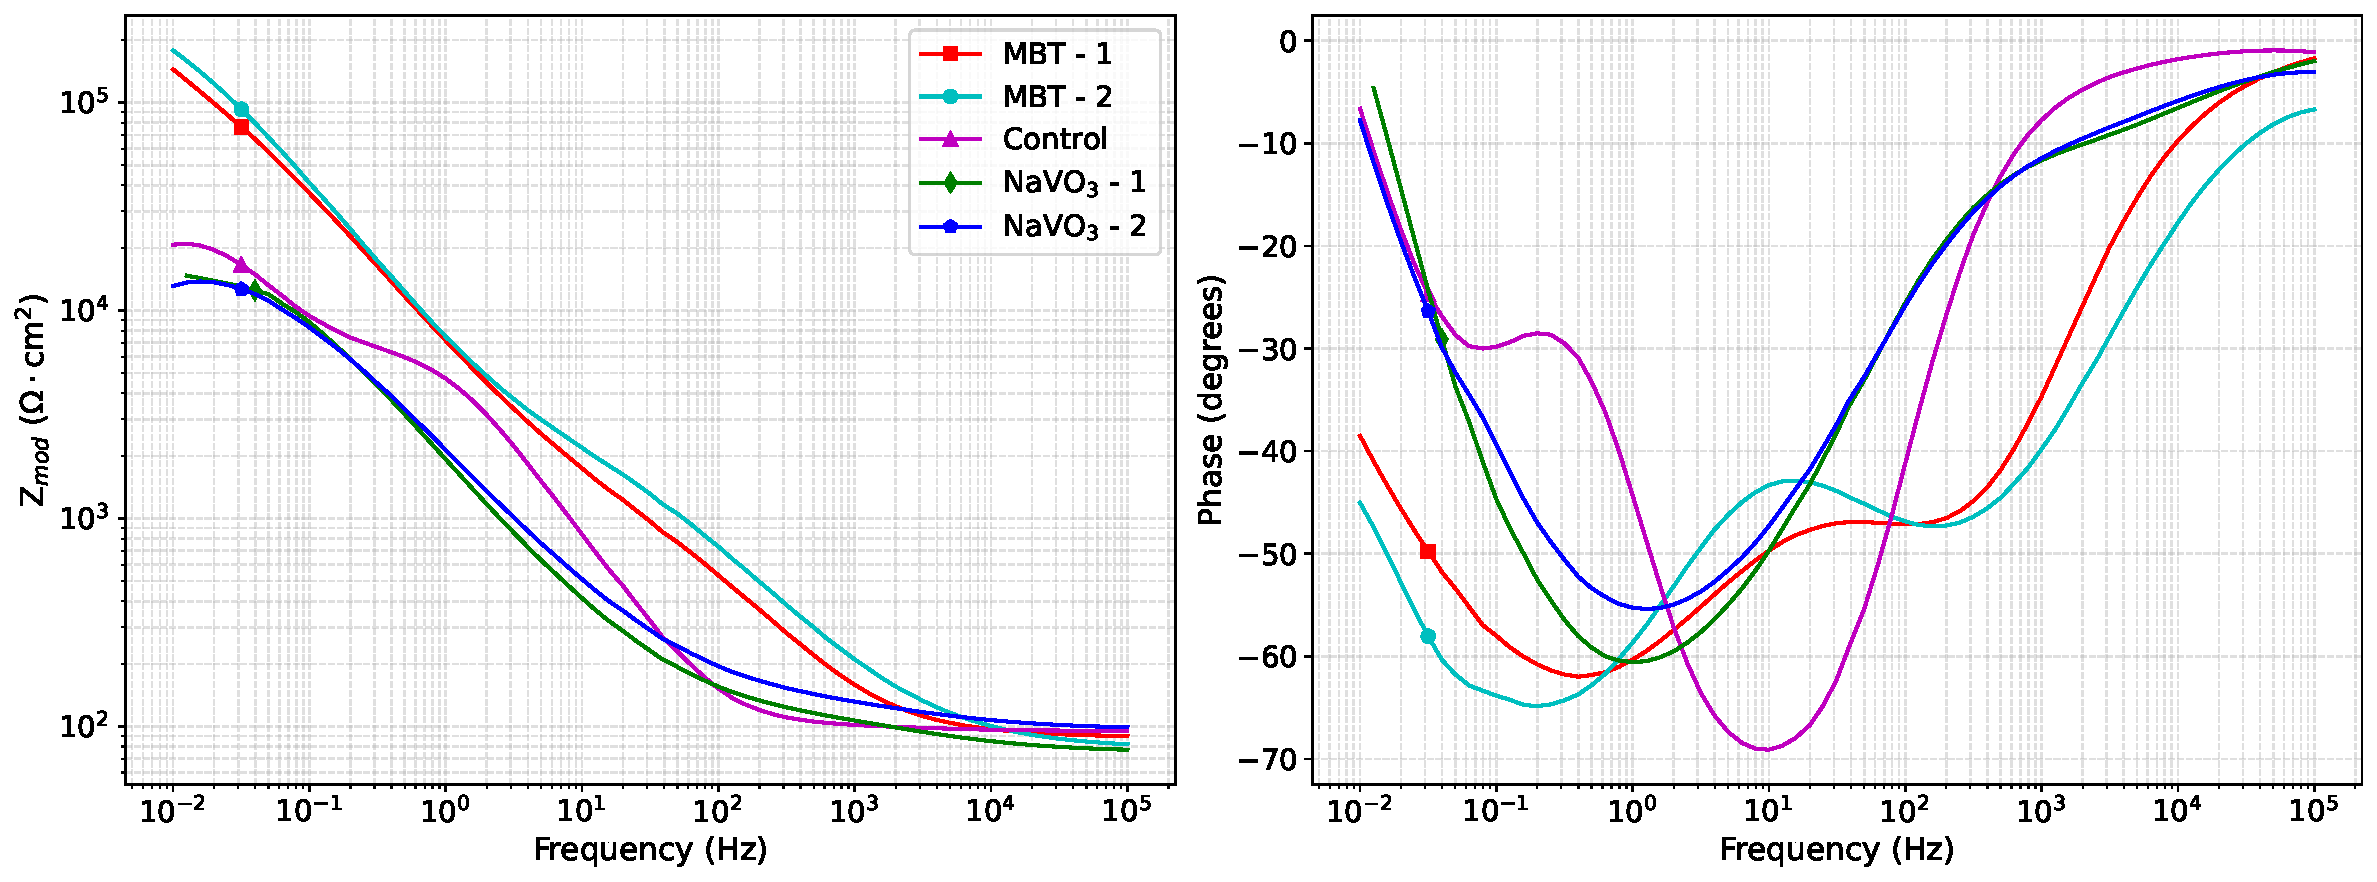
\includegraphics[width=\textwidth]{figs/bode_1H_LDH_2.pdf}
       \caption{\qty{1}{\hour} immersion.}
       \label{fig:ldh2_1h_bode}
   \end{subfigure}

   \vspace{0.3cm}

   \begin{subfigure}[b]{0.95\textwidth}
       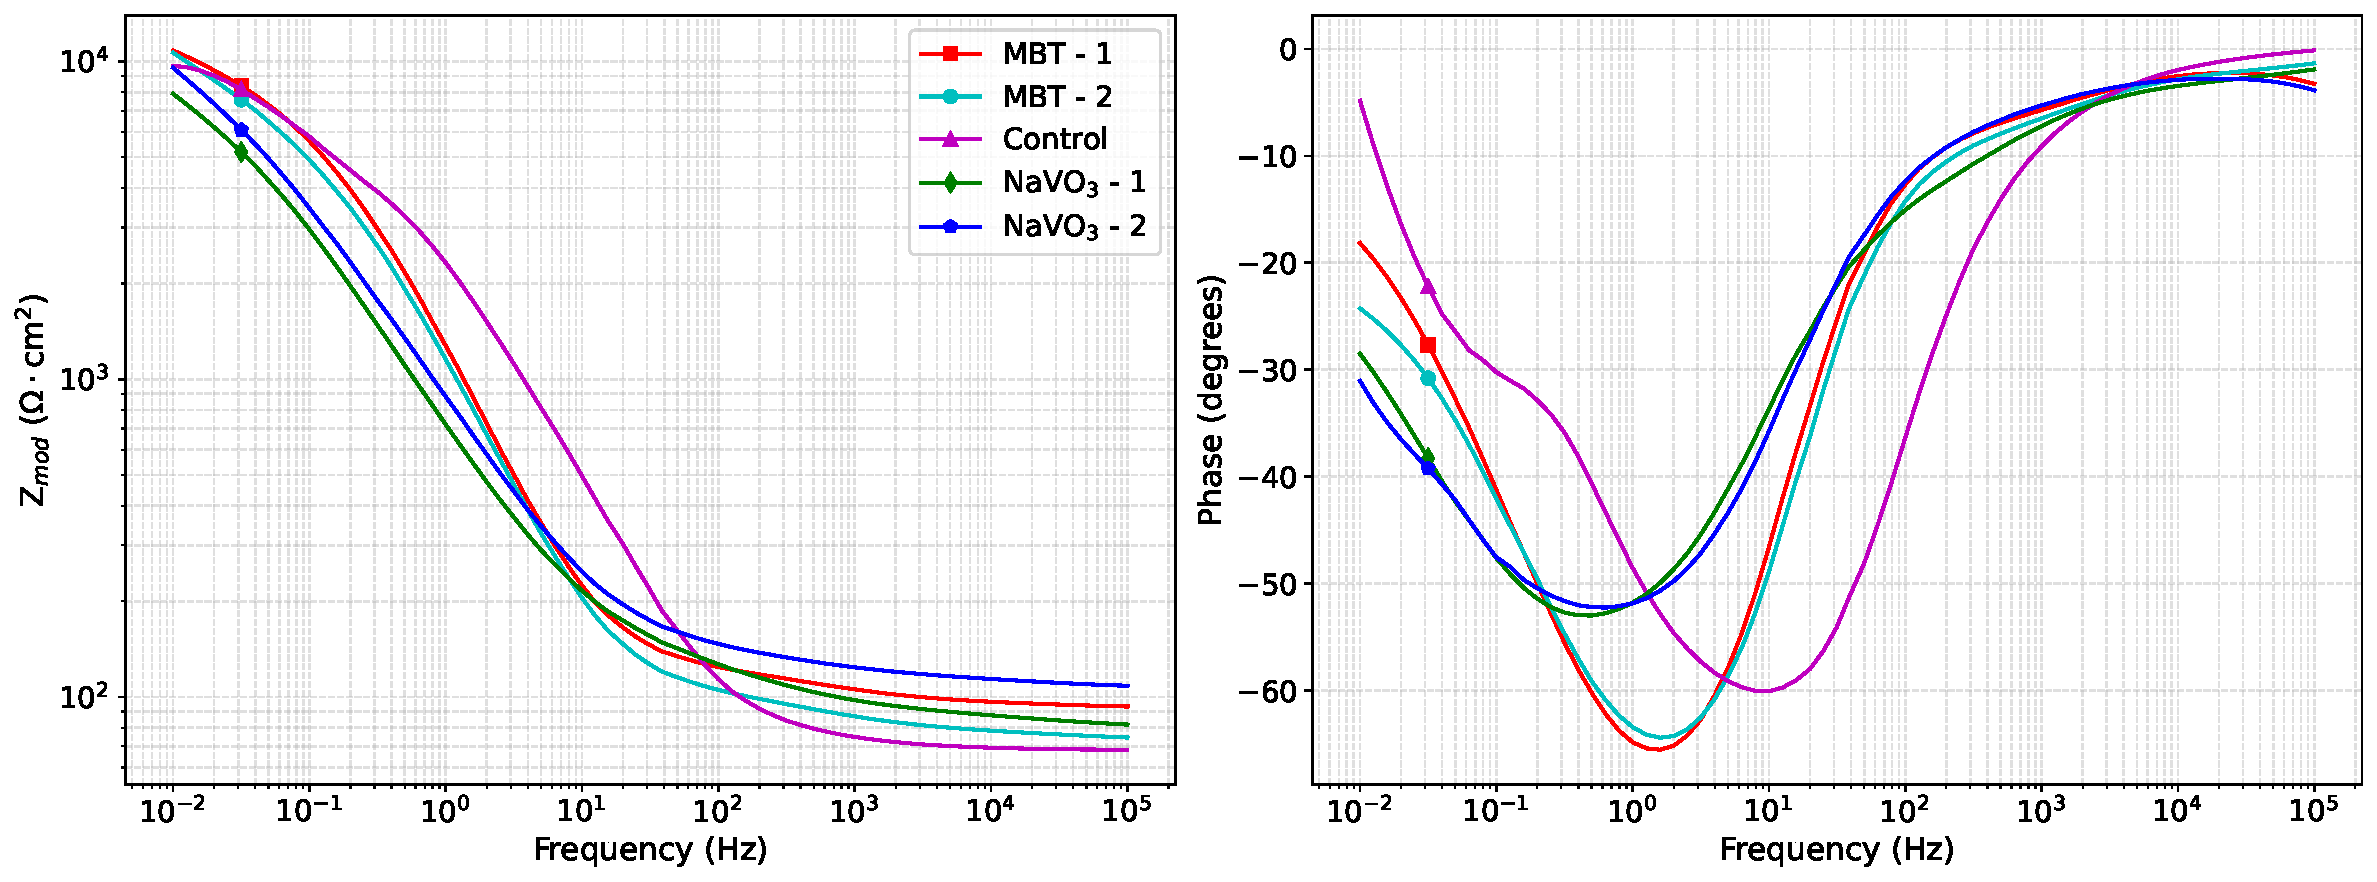
\includegraphics[width=\textwidth]{figs/bode_168H_LDH_2.pdf}
       \caption{\qty{168}{\hour} immersion.}
       \label{fig:ldh2_168h_bode}
   \end{subfigure}
   \caption{Bode spectra for LDH-2 specimens at \qty{1}{\hour} and 
   \qty{168}{\hour} of immersion in \qty{0.05}{\molar} \ce{NaCl}.}
   \label{fig:ldh2_bode}
\end{figure}

\begin{figure}[htbp]
   \centering
   \begin{subfigure}[b]{0.4\textwidth}
       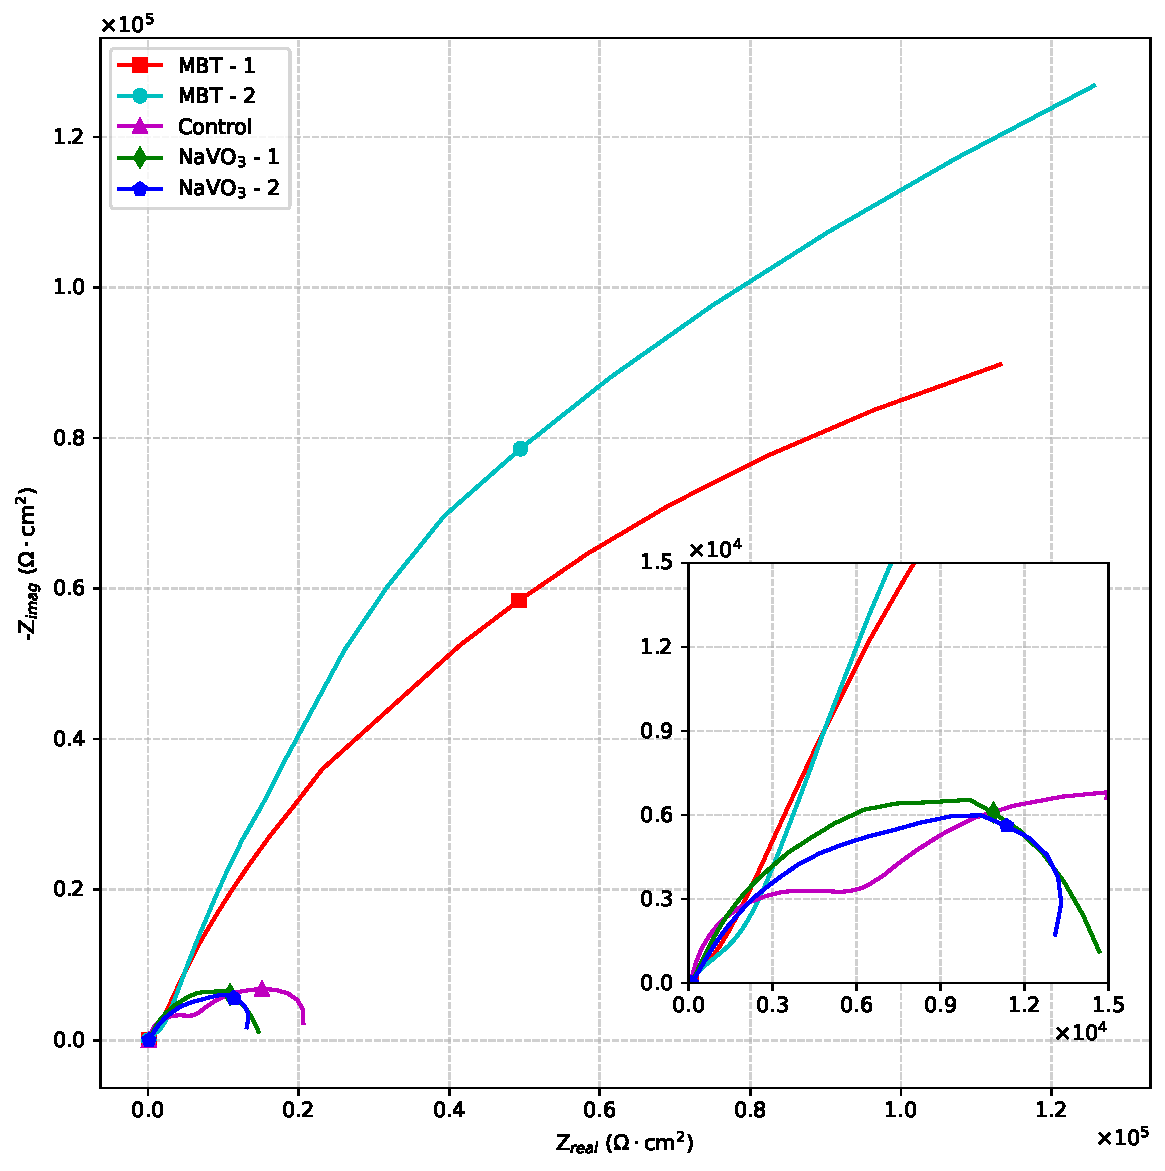
\includegraphics[width=\textwidth]{figs/nyquist_1H_LDH_2.pdf}
       \caption{\qty{1}{\hour} immersion.}
       \label{fig:ldh2_1h_nyquist}
   \end{subfigure}
   \begin{subfigure}[b]{0.4\textwidth}
       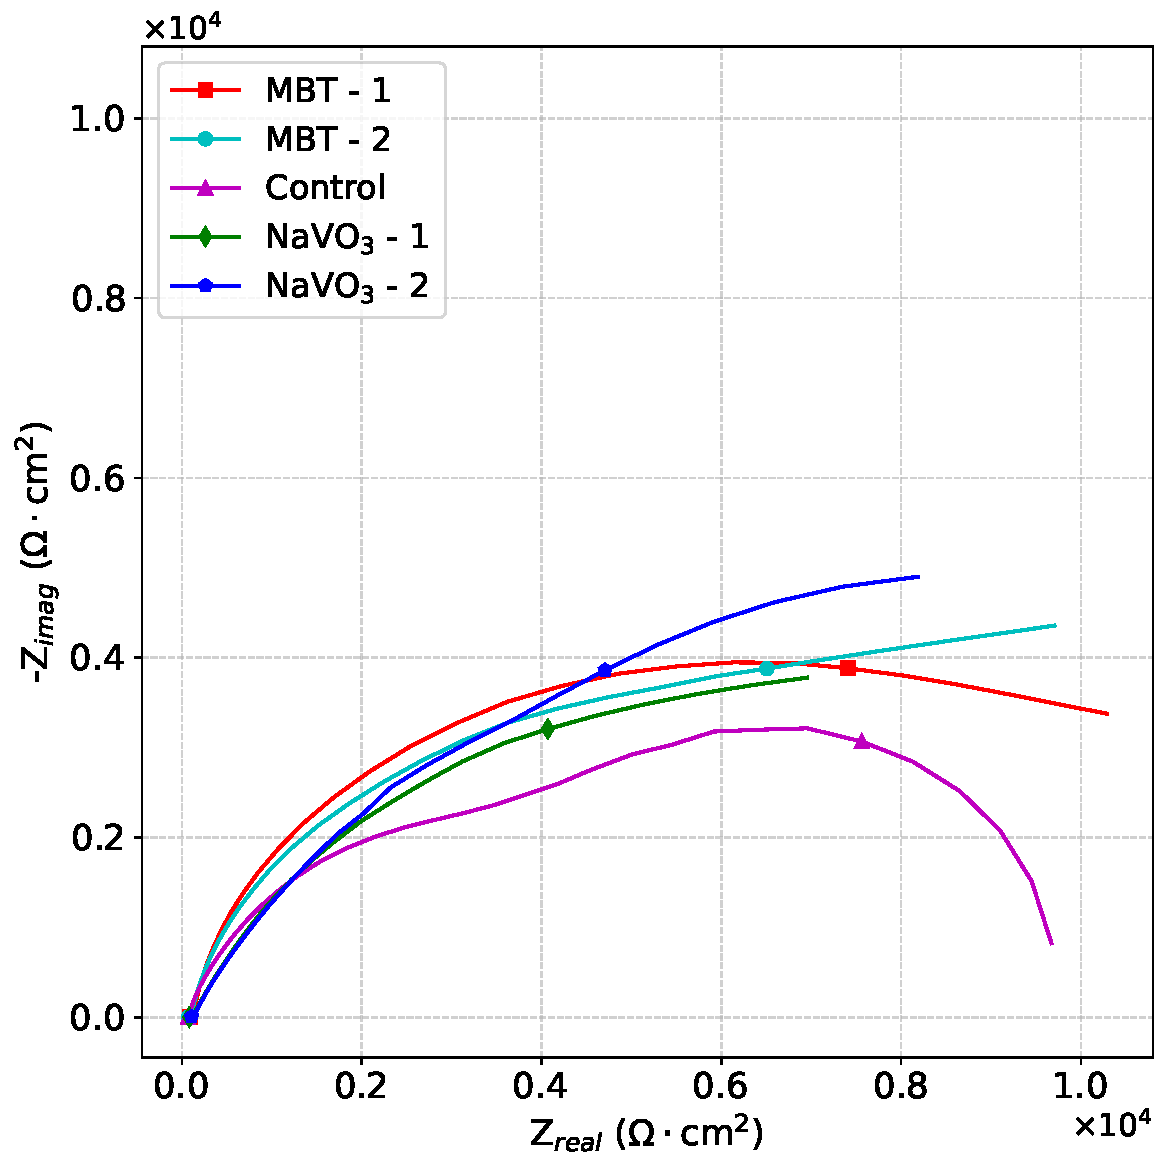
\includegraphics[width=\textwidth]{figs/nyquist_168H_LDH_2.pdf}
       \caption{\qty{168}{\hour} immersion.}
       \label{fig:ldh2_168h_nyquist}
   \end{subfigure}   
   \caption{Nyquist spectra for LDH-2 specimens at \qty{1}{\hour} and 
   \qty{168}{\hour} of immersion in \qty{0.05}{\molar} \ce{NaCl}.}
   \label{fig:ldh2_nyquist}
\end{figure}

The Bode and Nyquist spectra for LDH-2 are presented in Figures~\ref{fig:ldh2_bode} and~\ref{fig:ldh2_nyquist}. At \qty{1}{\hour} of immersion, the \ce{NaVO3}-intercalated specimens display a low-frequency impedance response comparable to the control, while the MBT-intercalated specimens exhibit a markedly superior response, with a low-frequency impedance modulus approximately one order of magnitude higher than both the control and vanadate systems. By \qty{168}{\hour}, however, the MBT systems show a progressive decline in impedance, converging towards values similar to those of the \ce{NaVO3} and control specimens, suggesting gradual inhibitor depletion or consumption over the immersion period.

\begin{figure}[htbp]
    \centering
    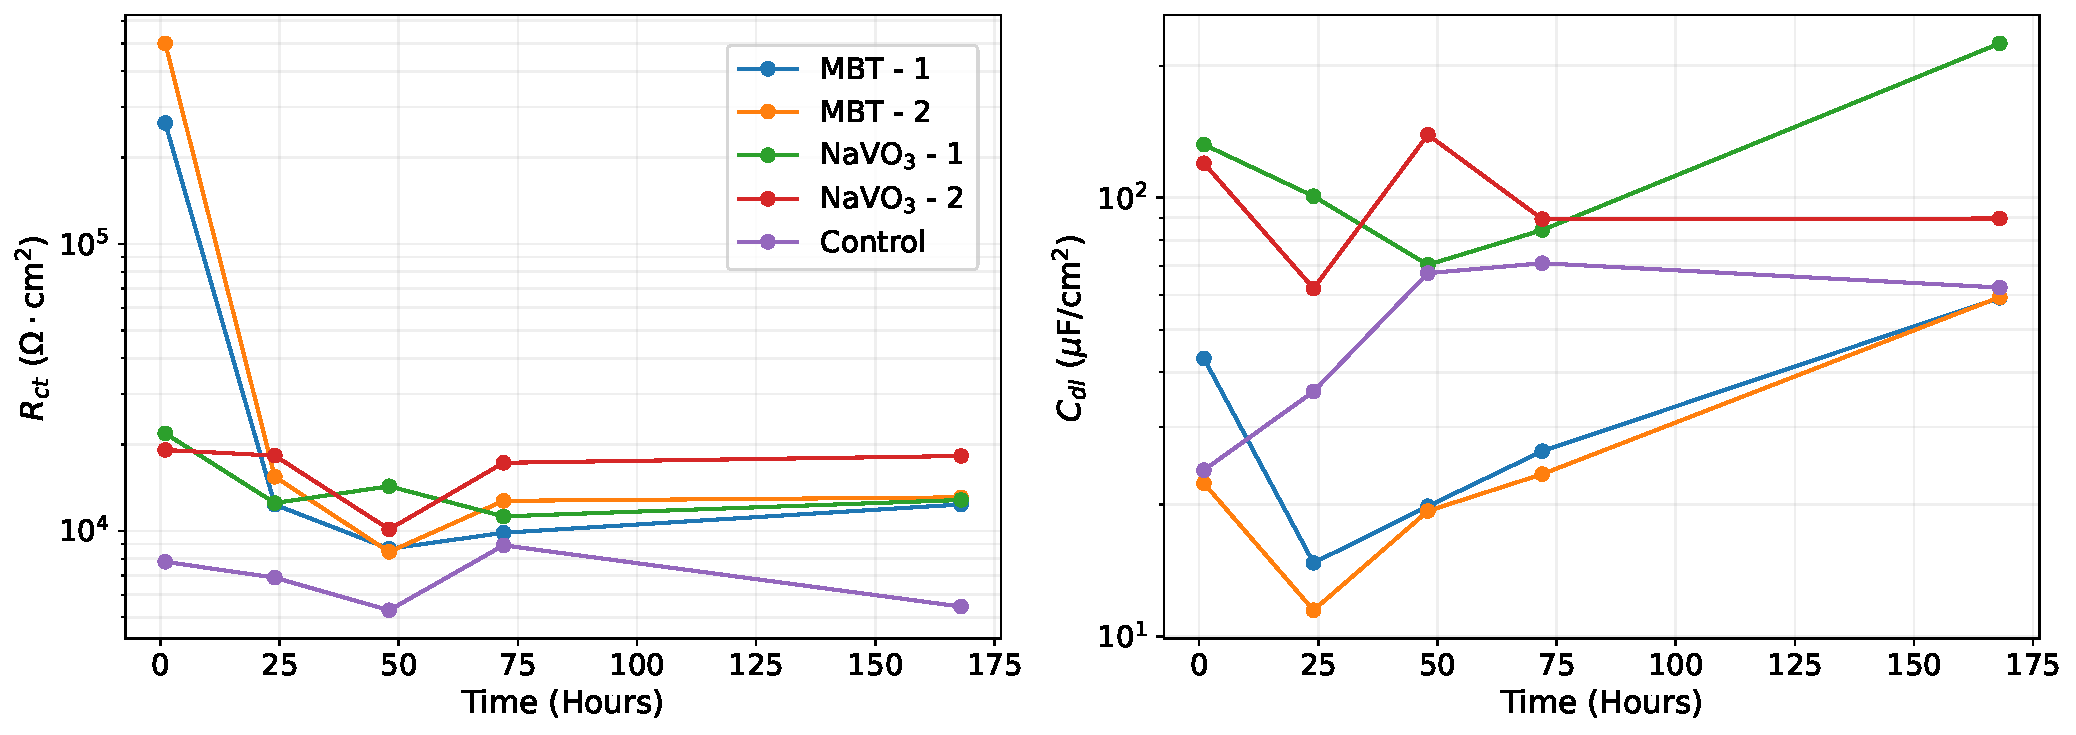
\includegraphics[width=0.95\textwidth]{figs/Rct_Cdl_evolution_LDH2.pdf} 
    \caption{Evolution of $R_{\text{ct}}$ and $C_{\text{dl}}$ as a function of 
    immersion time for LDH-2 specimens in \qty{0.05}{\molar} \ce{NaCl}.}
    \label{fig:Rct_Cdl_evolution_ldh2}
\end{figure}

The $R_{\text{ct}}$ and $C_{\text{dl}}$ evolution for LDH-2 is shown in Figure~\ref{fig:Rct_Cdl_evolution_ldh2}. The MBT-intercalated specimens exhibit substantially elevated $R_{\text{ct}}$ values at early immersion times, consistent with the high initial impedance observed in the Bode spectra; however, after approximately \qty{24}{\hour} of immersion, their $R_{\text{ct}}$ values decrease to levels comparable to those of the \ce{NaVO3} and control specimens. Notably, all LDH-2 coated systems retain a modest but consistent advantage over the control specimen at \qty{168}{\hour}: while the control exhibits an $R_{\text{ct}}$ below \qty{6}{\kilo\ohm\centi\meter\squared}, all inhibitor-loaded specimens maintain values exceeding \qty{10}{\kilo\ohm\centi\meter\squared}. With respect to $C_{\text{dl}}$, both vanadate-intercalated specimens consistently display higher capacitance than the control throughout the immersion period, remaining in the vicinity of 90~$\mu$F~cm$^{-2}$, which is indicative of a larger effective electrochemically active area. In contrast, both MBT-intercalated specimens exhibit lower $C_{\text{dl}}$ values than the control throughout the experiment, despite a gradual increasing trend that suggests the capacitance may exceed that of the control beyond \qty{168}{\hour}.

\begin{figure}[htbp]
    \centering
    \begin{subfigure}[b]{0.18\textwidth}
        
\includegraphics[width=\textwidth]{figs/optical_LDH2/control_before.jpg}
        \caption{Control}
        \label{fig:optical_ldh2_before_control}
    \end{subfigure}
    \hfill
    \begin{subfigure}[b]{0.18\textwidth}
        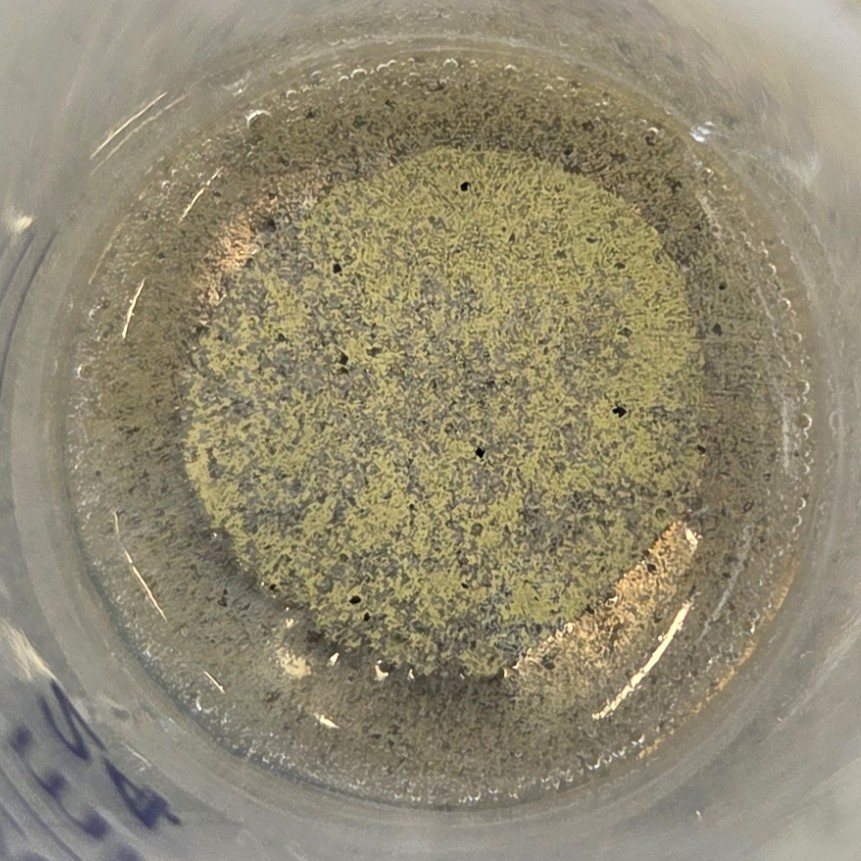
\includegraphics[width=\textwidth]{figs/optical_LDH2/MBT_1_before.jpg}
        \caption{MBT 1}
        \label{fig:optical_ldh2_before_1}
    \end{subfigure}
    \hfill
    \begin{subfigure}[b]{0.18\textwidth}
        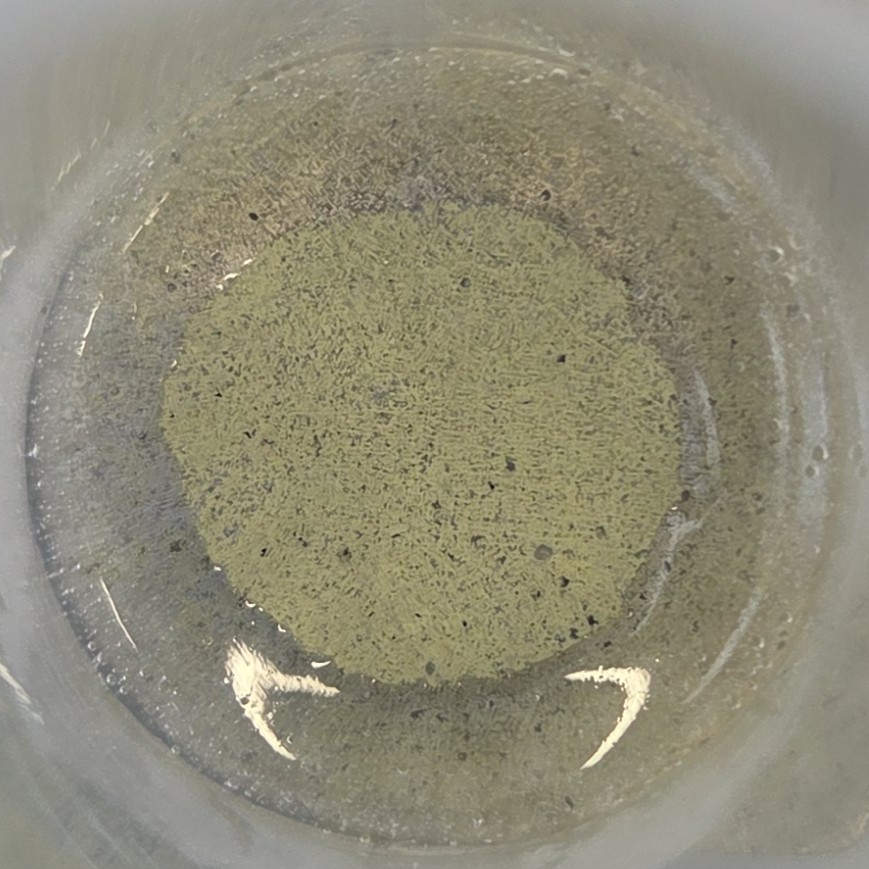
\includegraphics[width=\textwidth]{figs/optical_LDH2/MBT_2_before.jpg}
        \caption{MBT 2}
        \label{fig:optical_ldh2_before_2}
    \end{subfigure}
    \hfill
    \begin{subfigure}[b]{0.18\textwidth}
        
\includegraphics[width=\textwidth]{figs/optical_LDH2/NaVO3_1_before.jpg}
        \caption{\ce{NaVO3} 1}
        \label{fig:optical_ldh2_before_3}
    \end{subfigure}
    \hfill
    \begin{subfigure}[b]{0.18\textwidth}
        
\includegraphics[width=\textwidth]{figs/optical_LDH2/NaVO3_2_before.jpg}
        \caption{\ce{NaVO3} 2}
        \label{fig:optical_ldh2_before_4}
    \end{subfigure}

    \vspace{0.3cm}
    \begin{subfigure}[b]{0.18\textwidth}
        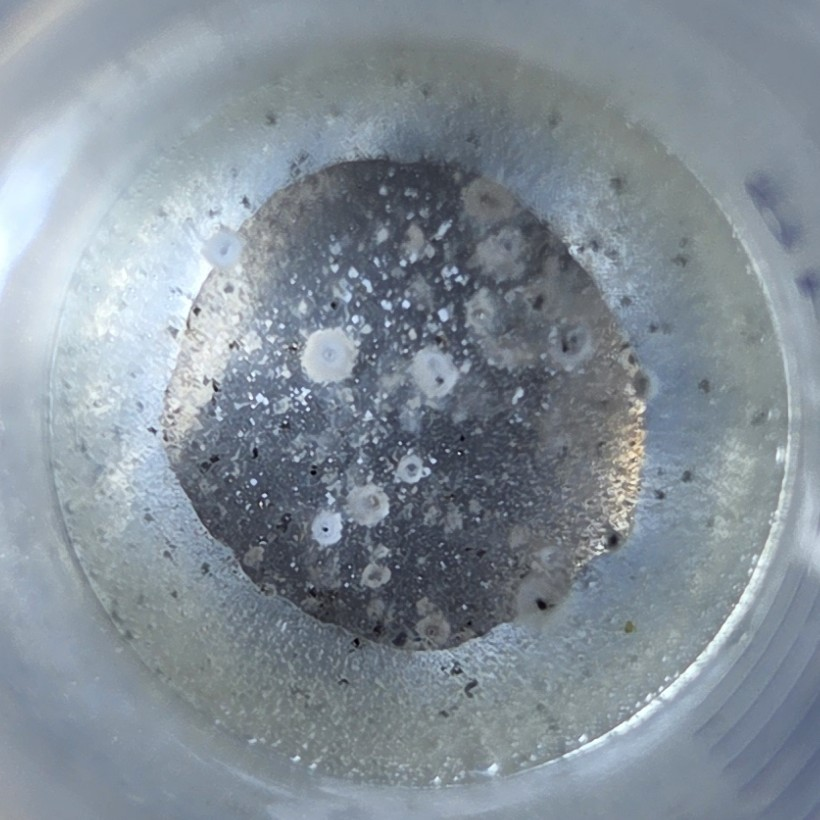
\includegraphics[width=\textwidth]{figs/optical_LDH2/control_72h.jpg}
        \caption{Control}
        \label{fig:optical_ldh2_72h_control}
    \end{subfigure}
    \hfill
    \begin{subfigure}[b]{0.18\textwidth}
        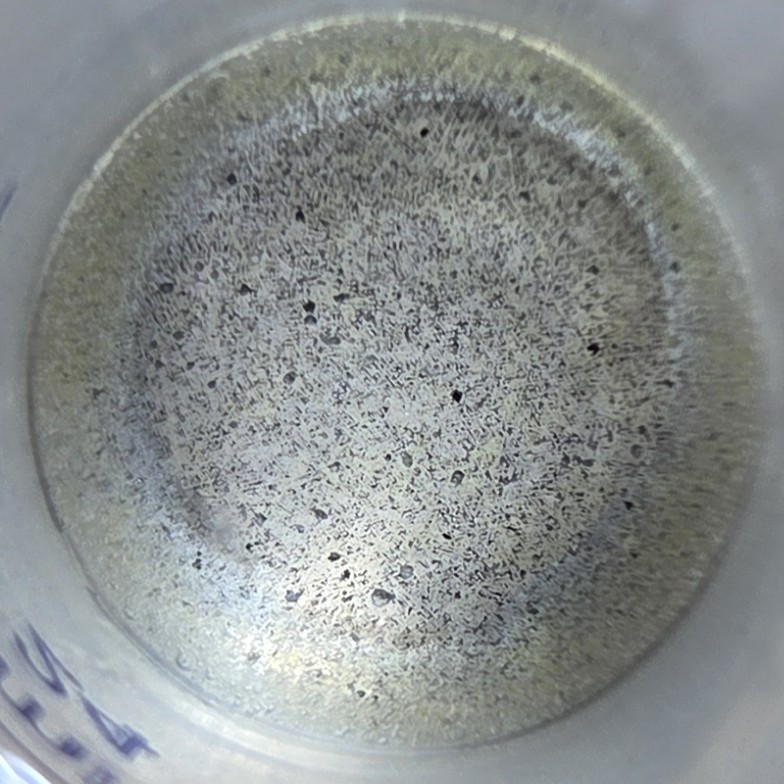
\includegraphics[width=\textwidth]{figs/optical_LDH2/MBT_1_72h.jpg}
        \caption{MBT 1}
        \label{fig:optical_ldh2_72h_1}
    \end{subfigure}
    \hfill
    \begin{subfigure}[b]{0.18\textwidth}
        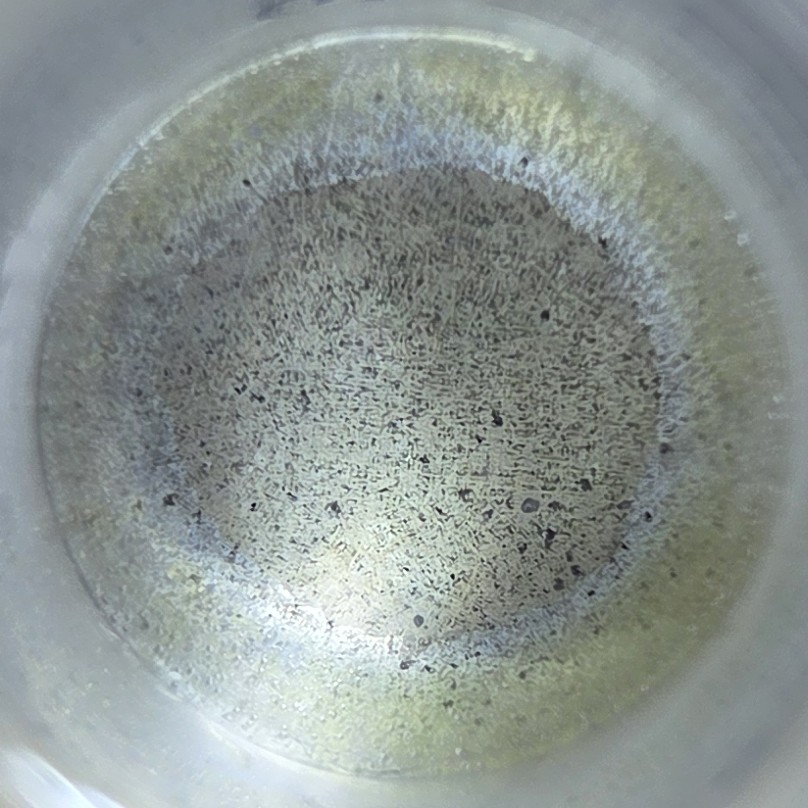
\includegraphics[width=\textwidth]{figs/optical_LDH2/MBT_2_72h.jpg}
        \caption{MBT 2}
        \label{fig:optical_ldh2_72h_2}
    \end{subfigure}
    \hfill
    \begin{subfigure}[b]{0.18\textwidth}
        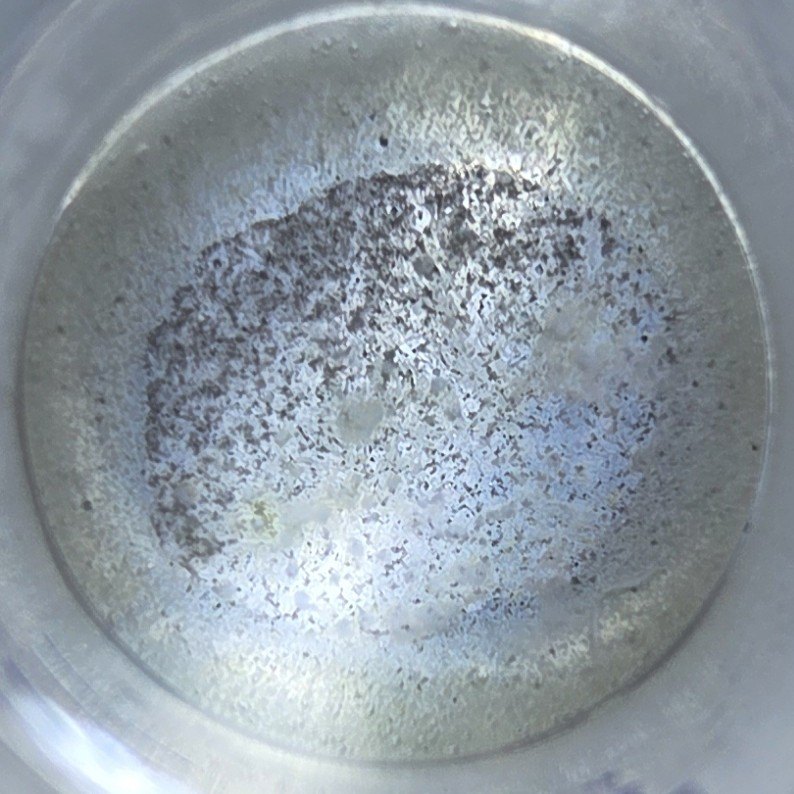
\includegraphics[width=\textwidth]{figs/optical_LDH2/NaVO3_1_72h.jpg}
        \caption{\ce{NaVO3} 1}
        \label{fig:optical_ldh2_72h_3}
    \end{subfigure}
    \hfill
    \begin{subfigure}[b]{0.18\textwidth}
        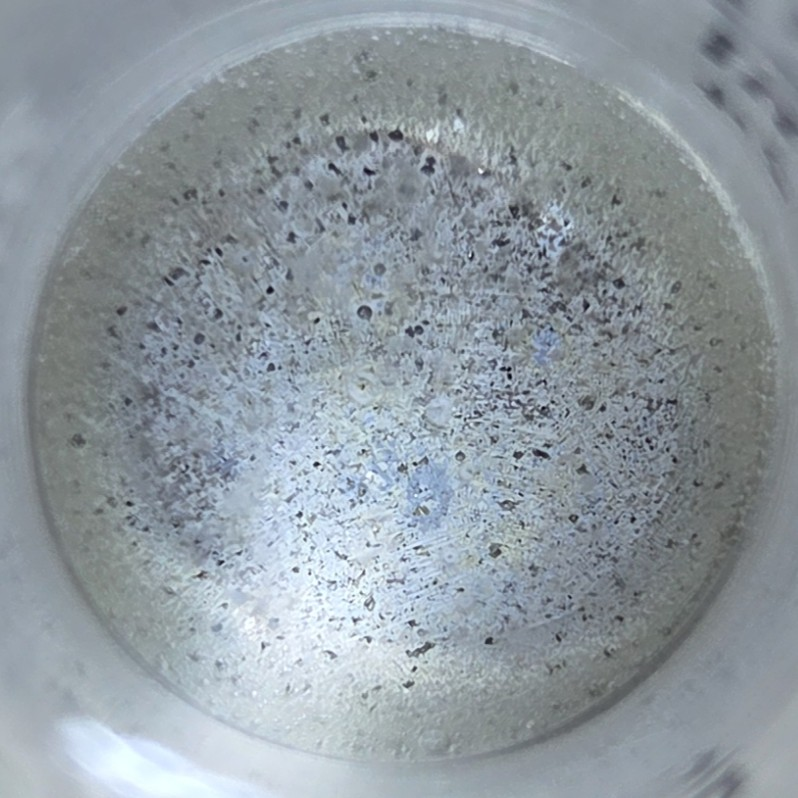
\includegraphics[width=\textwidth]{figs/optical_LDH2/NaVO3_2_72h.jpg}
        \caption{\ce{NaVO3} 2}
        \label{fig:optical_ldh2_72h_4}
    \end{subfigure}

    \vspace{0.3cm}
    \begin{subfigure}[b]{0.18\textwidth}
        
\includegraphics[width=\textwidth]{figs/optical_LDH2/control_after.jpg}
        \caption{Control}
        \label{fig:optical_ldh2_after_control}
    \end{subfigure}
    \hfill
    \begin{subfigure}[b]{0.18\textwidth}
        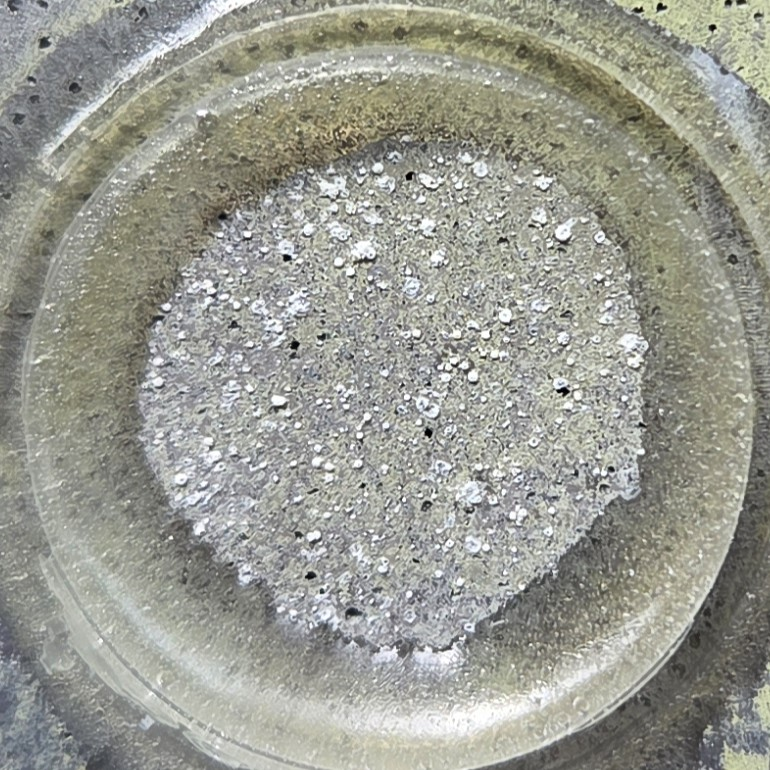
\includegraphics[width=\textwidth]{figs/optical_LDH2/MBT_1_after.jpg}
        \caption{MBT 1}
        \label{fig:optical_ldh2_after_1}
    \end{subfigure}
    \hfill
    \begin{subfigure}[b]{0.18\textwidth}
        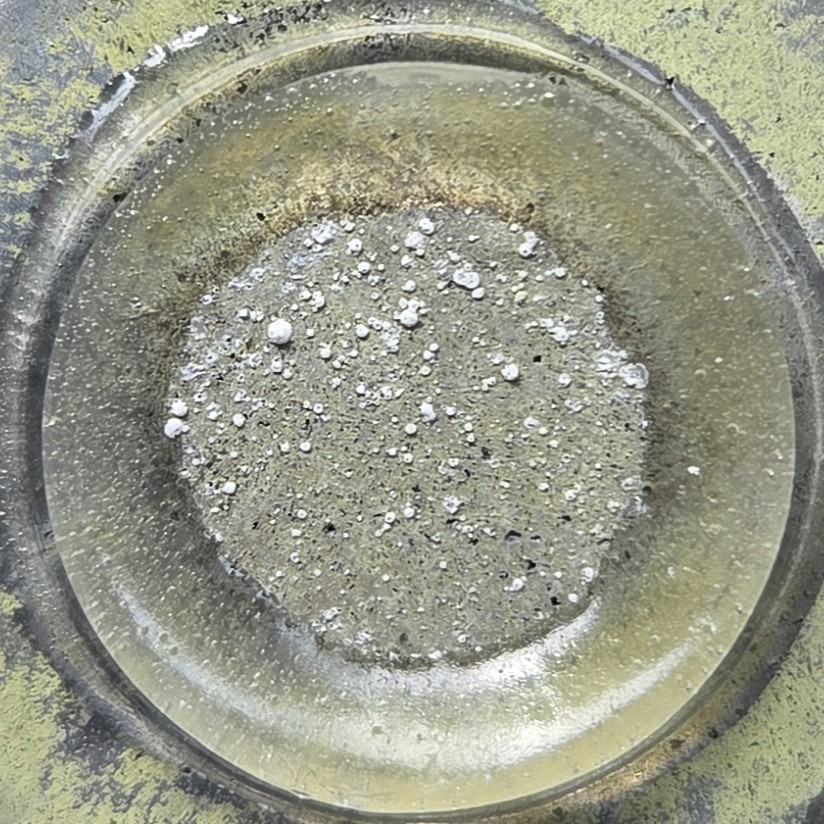
\includegraphics[width=\textwidth]{figs/optical_LDH2/MBT_2_after.jpg}
        \caption{MBT 2}
        \label{fig:optical_ldh2_after_2}
    \end{subfigure}
    \hfill
    \begin{subfigure}[b]{0.18\textwidth}
        
\includegraphics[width=\textwidth]{figs/optical_LDH2/NaVO3_1_after.jpg}
        \caption{\ce{NaVO3} 1}
        \label{fig:optical_ldh2_after_3}
    \end{subfigure}
    \hfill
    \begin{subfigure}[b]{0.18\textwidth}
        
\includegraphics[width=\textwidth]{figs/optical_LDH2/NaVO3_2_after.jpg}
        \caption{\ce{NaVO3} 2}
        \label{fig:optical_ldh2_after_4}
    \end{subfigure}
    \caption{Optical photographs of LDH-2 specimens at three stages of immersion in \qty{0.05}{\molar} \ce{NaCl}. Top row (a)--(e): prior to immersion. Middle row (f)--(j): after \qty{72}{\hour} of immersion. Bottom row (k)--(o): after \qty{168}{\hour} of immersion. (a,f,k)~Control, (b,g,l)~MBT~1, (c,h,m)~MBT~2, (d,i,n)~\ce{NaVO3}~1, (e,j,o)~\ce{NaVO3}~2.}
    \label{fig:optical_ldh2}
\end{figure}

Optical inspection of the LDH-2 specimens at three stages of immersion, presented in Figure~\ref{fig:optical_ldh2}, provides visual confirmation of the electrochemical trends described above. Prior to immersion, the \ce{NaVO3}-intercalated specimens (Figures~\ref{fig:optical_ldh2_before_3} and~\ref{fig:optical_ldh2_before_4}) display visible surface heterogeneities in the LDH film, with areas of incomplete substrate coverage, which may partially account for their comparatively weaker electrochemical performance relative to the MBT-intercalated specimens.

At \qty{72}{\hour} of immersion, a clear differentiation between the inhibitor systems is already apparent, consistent with the electrochemical parameters extracted at this time point. The MBT-intercalated specimens display a homogeneous surface with no visible signs of pitting or generalised corrosion, in agreement with the substantially lower $C_{\text{dl}}$ values recorded for these specimens at \qty{72}{\hour} (20--30~$\mu$F~cm$^{-2}$ compared to approximately 70~$\mu$F~cm$^{-2}$ for the control), indicating that the LDH coating remains largely intact and water uptake has not yet occurred to a significant extent. The \ce{NaVO3}-intercalated specimens, while not exhibiting discrete pits at this stage, already show a diffuse whitish surface appearance indicative of incipient generalised aluminium matrix corrosion, consistent with their $C_{\text{dl}}$ values being comparable to those of the control at this time point. The control specimen, by contrast, already displays significant discrete pitting at \qty{72}{\hour}, confirming that the inhibitor-loaded systems provide measurably superior corrosion protection even at intermediate immersion times.

Following \qty{168}{\hour} of immersion, the control specimen exhibits the most severe surface degradation, characterised by large discrete pits and extensive generalised aluminium matrix dissolution. The MBT-intercalated specimens present the best overall surface condition, with only minor pitting and a generalised yellowish surface deposit, the precise composition of which was not characterised in this work but is likely associated with the surface interaction products of MBT with dissolved metal species. The \ce{NaVO3}-intercalated specimens display an intermediate level of degradation --- superior to the control but inferior to the MBT systems --- with moderate pitting distributed across the surface alongside localised yellowish deposits characteristic of vanadium oxide precipitation at pit sites, confirming that vanadate release and repassivation did occur, albeit insufficiently to fully suppress corrosion progression over the full immersion period. These visual observations are fully consistent with the $R_{\text{ct}}$ and $C_{\text{dl}}$ trends discussed above and corroborate the ranking of inhibitor performance established by the electrochemical analysis.

\begin{figure}[htbp]
    \centering
    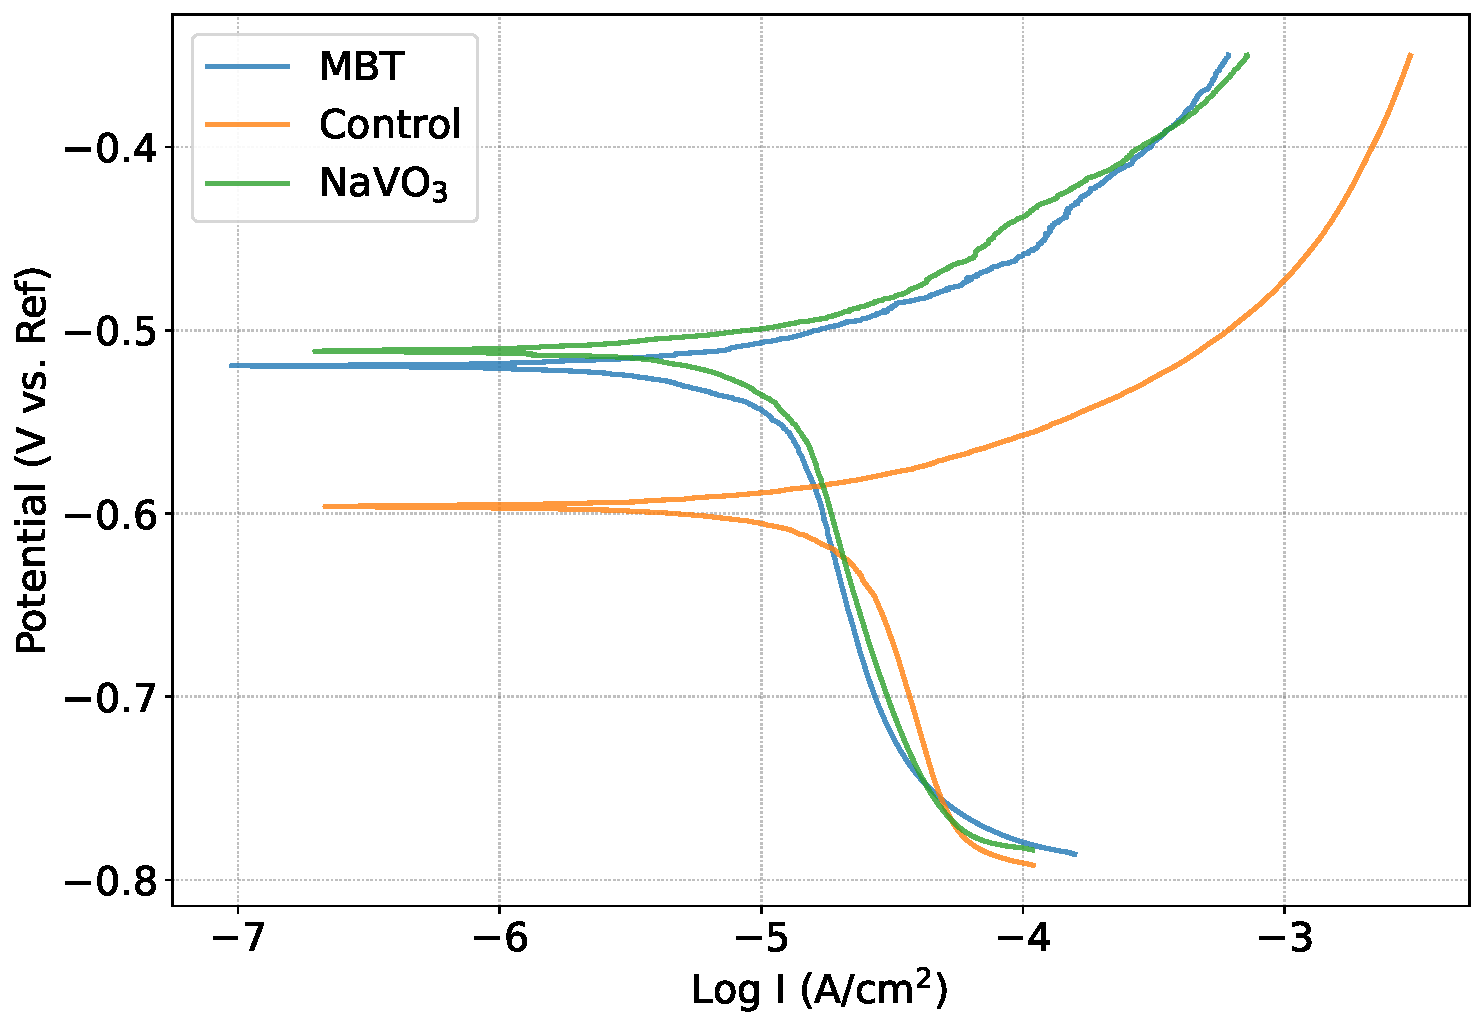
\includegraphics[width=0.5\textwidth]{figs/tafel_curves.pdf}
    \caption{Potentiodynamic polarisation curves for LDH-2 specimens following 
    \qty{168}{\hour} of immersion in \qty{0.05}{\molar} \ce{NaCl}.}
    \label{fig:pdp}
\end{figure}

The potentiodynamic polarisation curves for the LDH-2 specimens following \qty{168}{\hour} of immersion are presented in Figure~\ref{fig:pdp}. The cathodic branches of all three specimens are virtually superimposed, confirming that neither \ce{NaVO3} nor MBT is effective at suppressing the cathodic activity of the Fe--Mn and Cu-rich intermetallic sites that drive oxygen reduction in this system, as discussed in Section~\ref{sec:results_pretreatments}. In contrast, a clear differentiation is observed in the anodic branches, where the inhibitor-intercalated specimens exhibit measurably lower anodic current densities than the control, indicating that both inhibitor systems retard anodic dissolution of the aluminium matrix to a significant extent. The $E_{\text{corr}}$ values of the \ce{NaVO3} and MBT specimens are both shifted in the noble direction relative to the control, consistent with partial anodic inhibition reducing the equilibrium between anodic and cathodic partial reactions.

While the LDH-2 batch represents a clear improvement over LDH-1, the overall corrosion protection performance remains below the target level, attributed primarily to the persistence of Fe--Mn intermetallic particles on the chemically pre-treated surface. Unlike Cu-rich particles, which are the primary targets of vanadate and MBT inhibitors \cite{Tedim2011, Zhang2015}, the Fe--Mn IMPs characteristic of AC46000 are not effectively passivated by either inhibitor system, and their continued cathodic activity sustains localised corrosion that the inhibitor loading within the LDH galleries is insufficient to fully suppress.

\section{Top Coating and Complex Geometries}
\label{sec:results_topcoat}

Following the successful deposition of the inhibitor-intercalated LDH conversion coating, a water-based polyurethane colloidal formulation was applied to both planar and geometrically complex specimens via anodic electrodeposition, as described in Section~\ref{sec:topcoat}. The resulting coating systems were evaluated by optical inspection, cross-sectional SEM-EDS analysis, and Elcometer thickness measurements.

\begin{figure}[htbp]
    \centering
    \begin{subfigure}[b]{0.2\textwidth}
        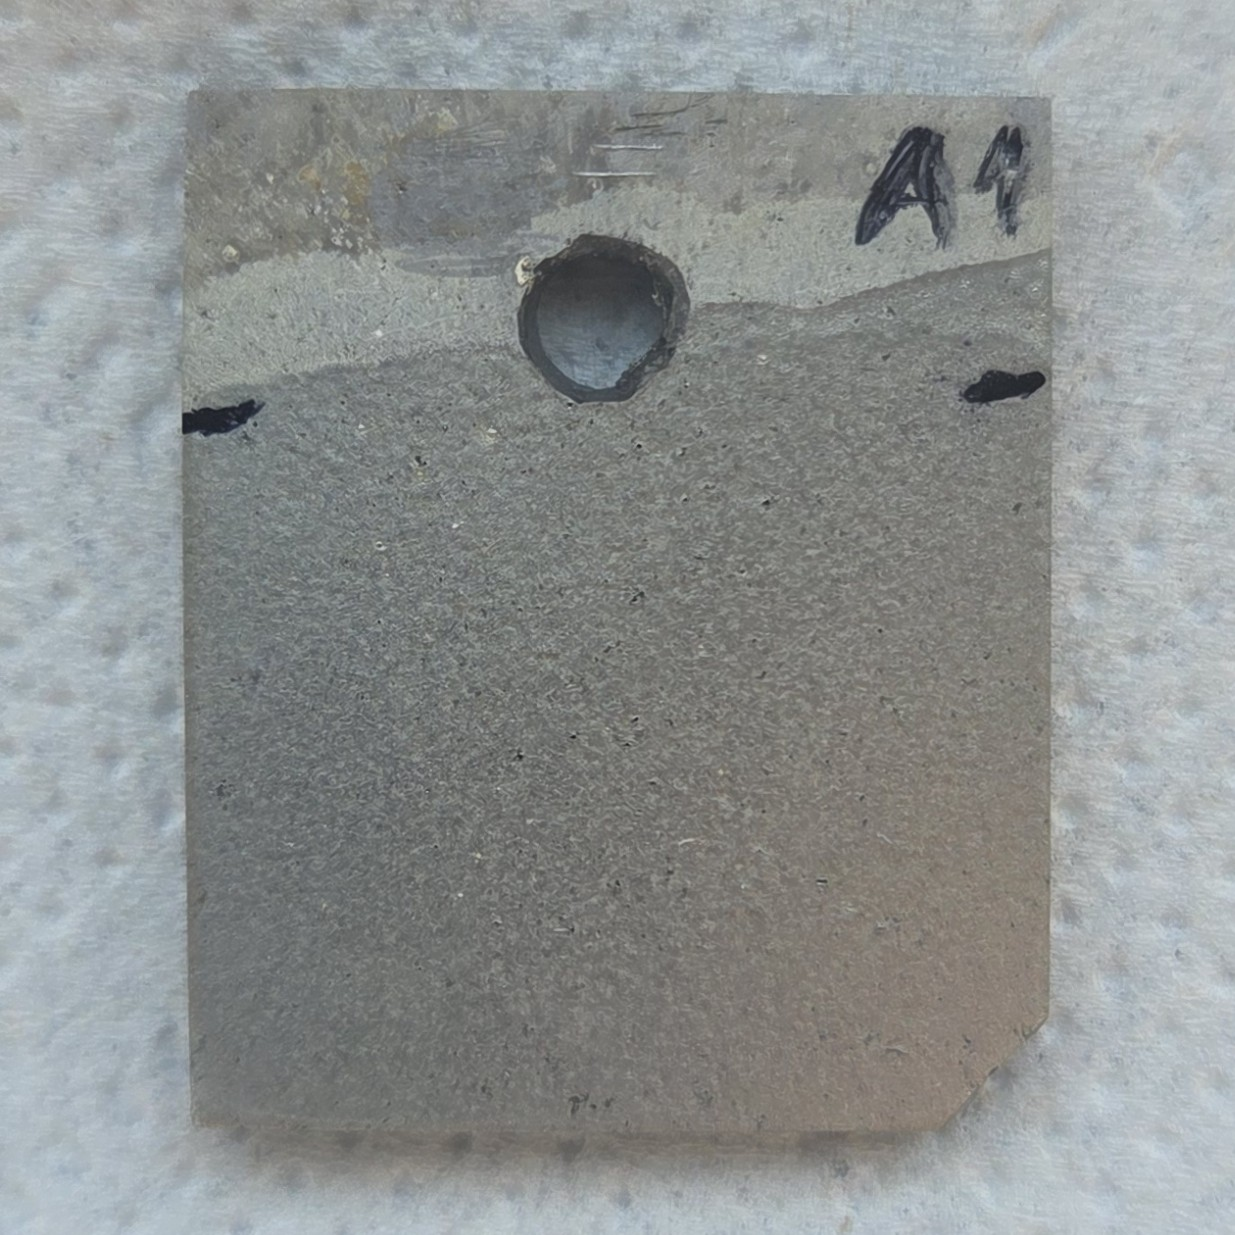
\includegraphics[width=\textwidth]{figs/topcoat/planar_MBT.jpg}
        \caption{Planar MBT}
        \label{fig:topcoat_planar_MBT}
    \end{subfigure}
    \begin{subfigure}[b]{0.2\textwidth}
        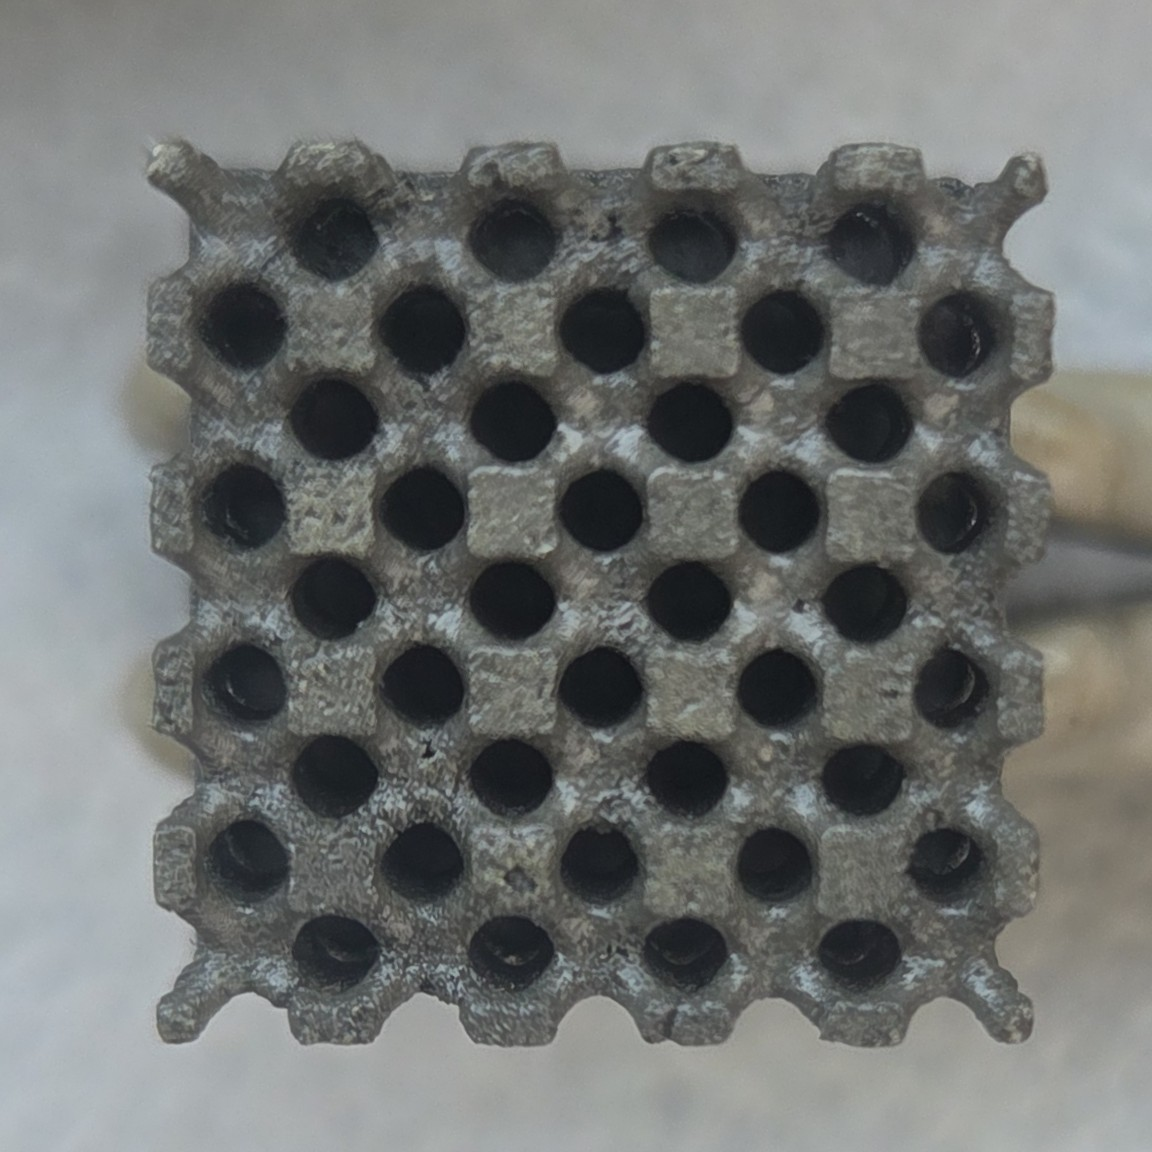
\includegraphics[width=\textwidth]{figs/topcoat/cg_MBT_1.jpg}
        \caption{CG MBT 1}
        \label{fig:topcoat_cg_MBT_1}
    \end{subfigure}
    \begin{subfigure}[b]{0.2\textwidth}
        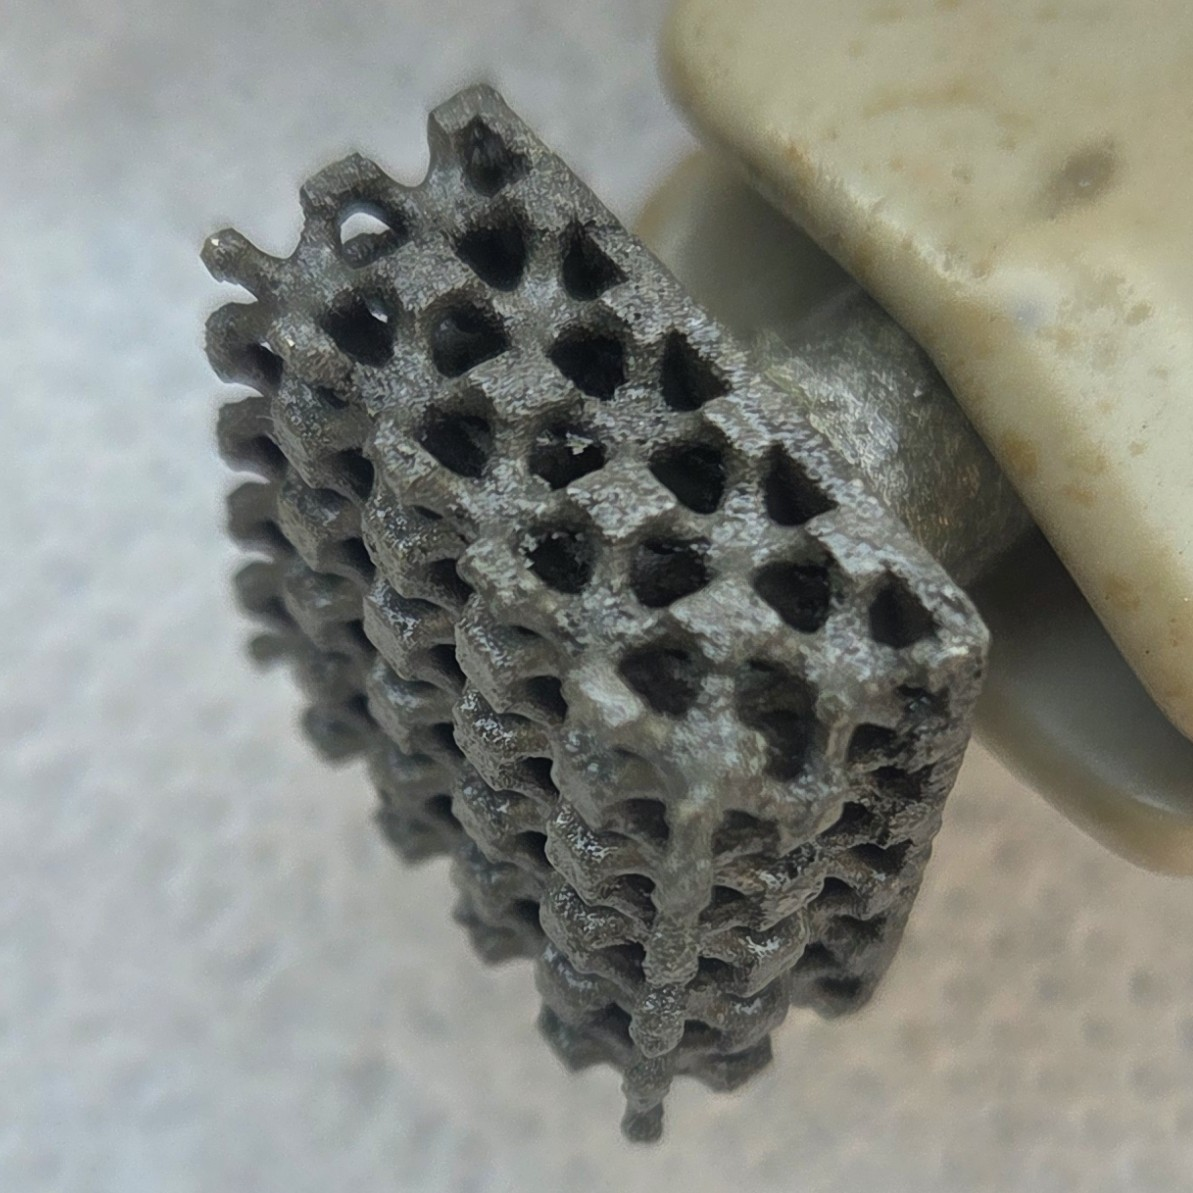
\includegraphics[width=\textwidth]{figs/topcoat/cg_MBT_2.jpg}
        \caption{CG MBT 2}
        \label{fig:topcoat_cg_MBT_2}
    \end{subfigure}
    \\
    \vspace{0.3cm}
    \begin{subfigure}[b]{0.2\textwidth}
        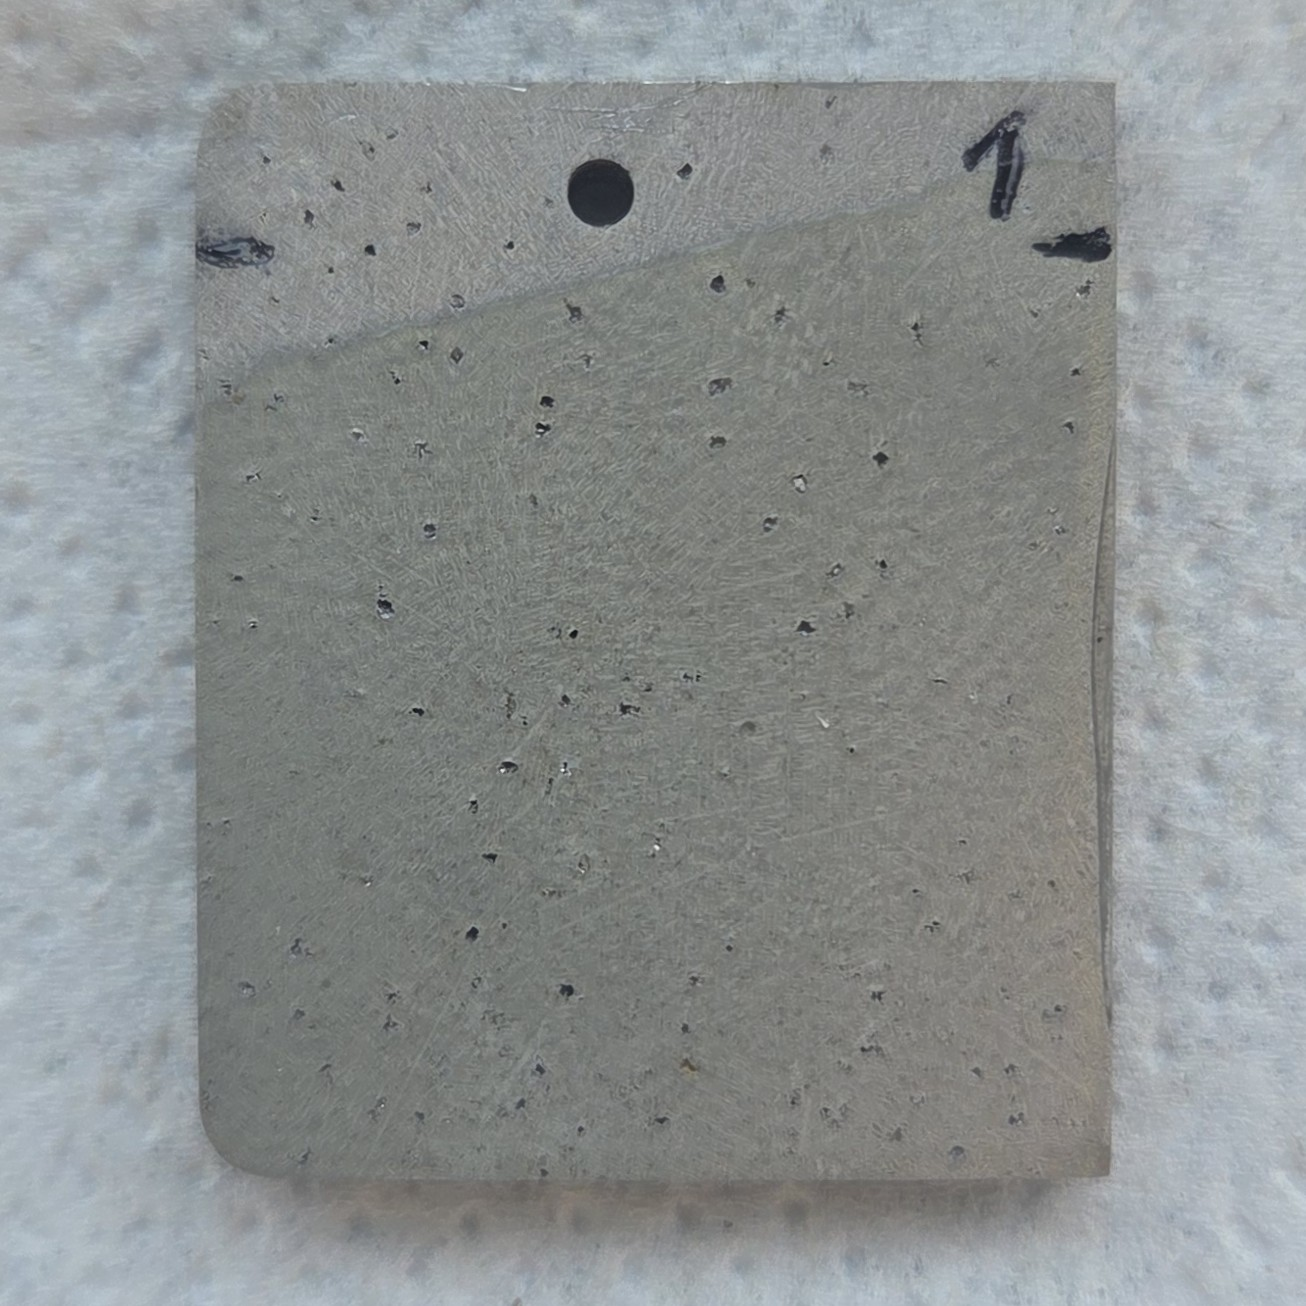
\includegraphics[width=\textwidth]{figs/topcoat/planar_NaVO3.jpg}
        \caption{Planar \ce{NaVO3}}
        \label{fig:topcoat_planar_NaVO3}
    \end{subfigure}
    \begin{subfigure}[b]{0.2\textwidth}
        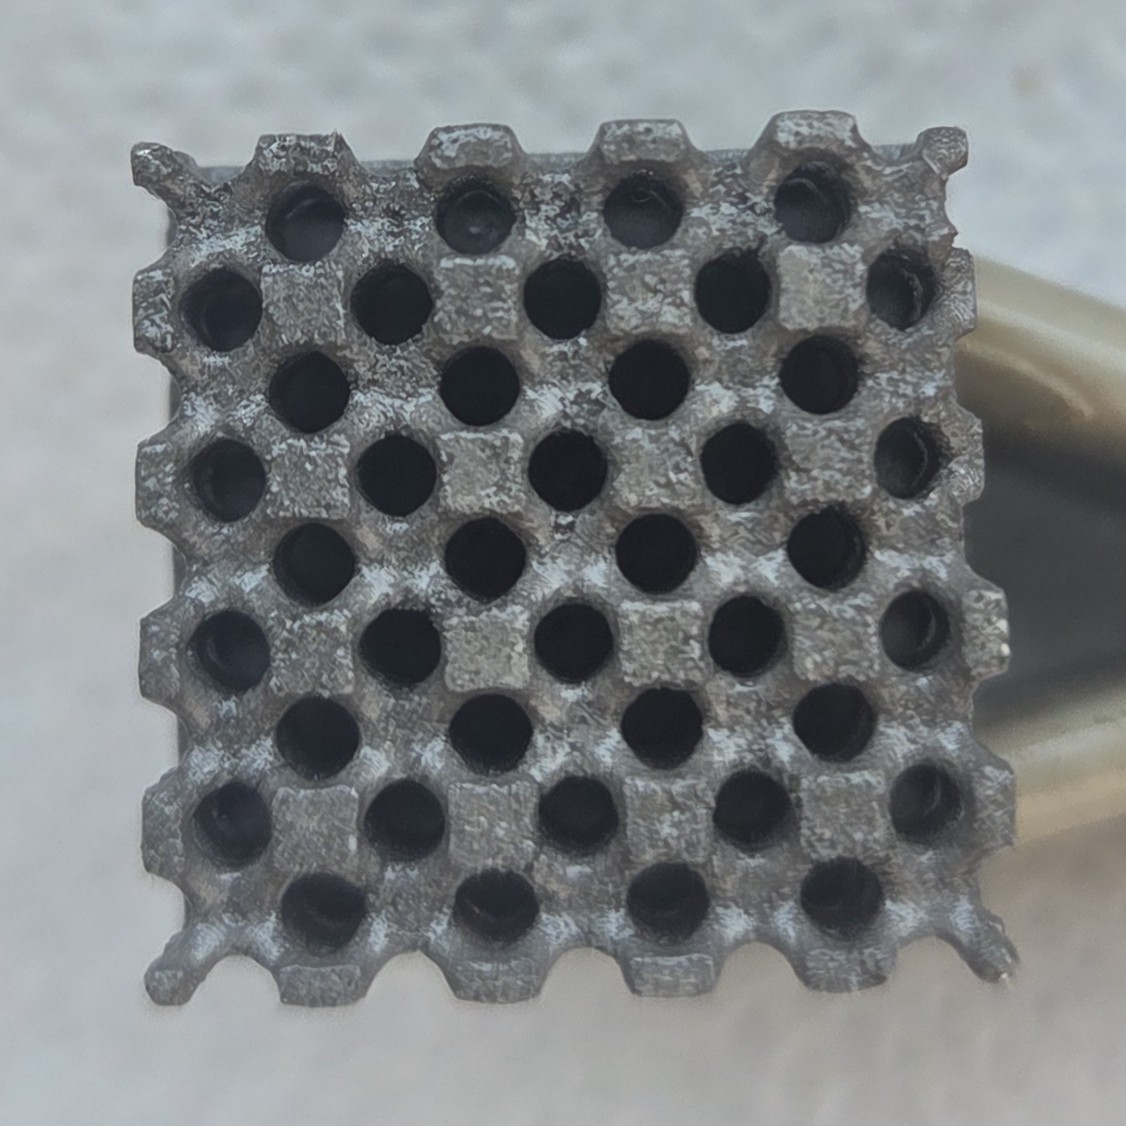
\includegraphics[width=\textwidth]{figs/topcoat/cg_NaVO3_1.jpg}
        \caption{CG \ce{NaVO3} 1}
        \label{fig:topcoat_cg_NaVO3_1}
    \end{subfigure}
    \begin{subfigure}[b]{0.2\textwidth}
        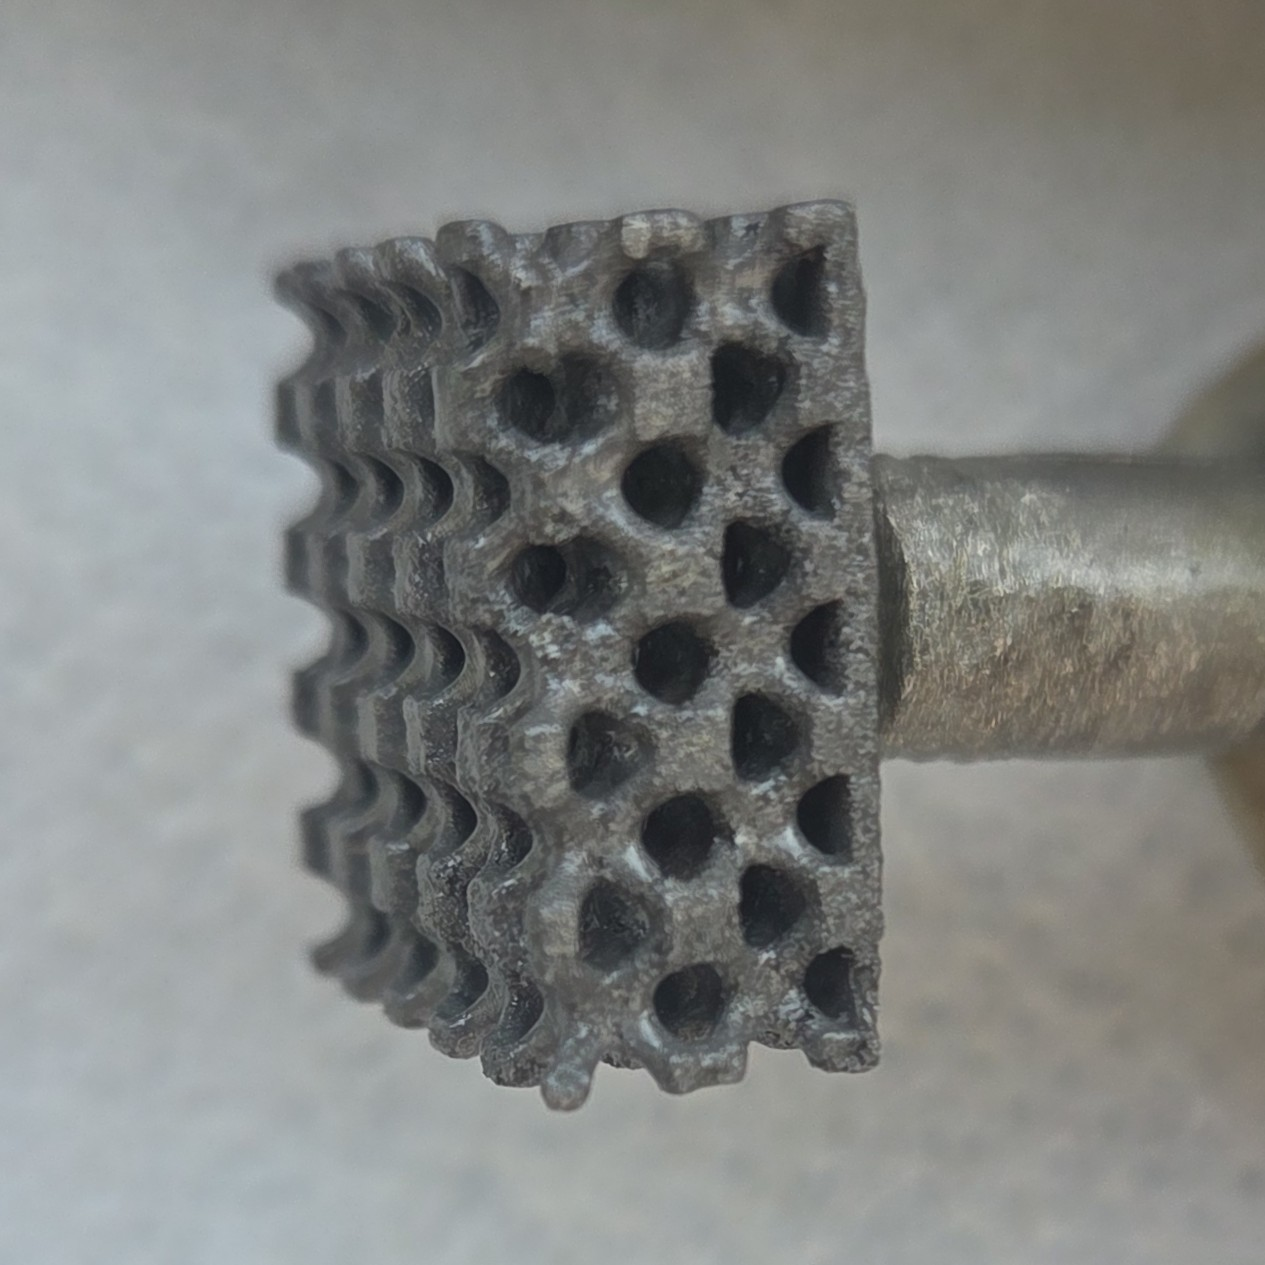
\includegraphics[width=\textwidth]{figs/topcoat/cg_NaVO3_2.jpg}
        \caption{CG \ce{NaVO3} 2}
        \label{fig:topcoat_cg_NaVO3_2}
    \end{subfigure}
    \caption{Optical photographs of polyurethane-coated specimens following 
    anodic electrodeposition and curing. Top row (a)--(c): MBT-intercalated 
    specimens. Bottom row (d)--(f): \ce{NaVO3}-intercalated specimens. 
    Left column: planar substrates. Centre and right columns: geometrically 
    complex substrates.}
    \label{fig:optical_topcoat}
\end{figure}

Optical inspection of the coated specimens, presented in Figure~\ref{fig:optical_topcoat}, confirms that the polyurethane topcoat forms a uniform and continuous film across all specimens for both planar and geometrically complex substrates, demonstrating that the anodic electrodeposition process is capable of conformally coating non-planar geometries. One notable observation is the presence of surface pores visible on the planar \ce{NaVO3} specimen (Figure~\ref{fig:topcoat_planar_NaVO3}), attributed to pre-existing macroscopic porosity in the die-cast substrate rather than to the deposition process itself: the casting process inherently generates gas porosity and shrinkage voids, and where these defects intersect the surface they present cavities of sufficient size that the polyurethane film is unable to bridge them completely.

To further characterise the multilayer system, cross-sections of the coated planar specimens were prepared by cutting and examined by SEM-EDS analysis, and coating thickness was measured using an Elcometer gauge. During the cutting procedure, no delamination was observed at the cut edges, confirming good interfacial adhesion between the polyurethane topcoat and the underlying LDH conversion coating. The cross-sectional SEM-EDS results are presented in Figures~\ref{fig:} to~\ref{fig:}. EDS elemental mapping across the cross-section reveals the spatial distribution of the constituent elements of each layer and provides insight into the degree of interpenetration between the polyurethane topcoat and the LDH film at their interface. Coating thickness measurements are summarised in Table~\ref{tab:thickness}.

[Discussion of SEM-EDS cross-section and thickness results to be added.]

\chapter{Conclusion \& Future Work}

\section{Conclusion}

This work investigated the synthesis, optimisation, and corrosion protection performance of ZnAl--LDH conversion coatings loaded with corrosion inhibitors on the AC46000 die-cast aluminium alloy, with the ultimate aim of validating the system on geometrically complex substrates as a chromate-free alternative for aerospace applications.

A pre-selection of corrosion inhibitors was first conducted by evaluating seven candidate systems via EIS over \qty{168}{\hour} of immersion in \qty{0.05}{\molar} \ce{NaCl}. MBT, \ce{NaVO3}, and L-cysteine were identified as the best-performing inhibitors, demonstrating $R_{\text{ct}}$ values in excess of \qty{100}{\kilo\ohm} and stable $C_{\text{dl}}$ values in the order of \qty{10}{\micro\farad} throughout the immersion period, indicative of active and durable film formation. Sodium molybdate provided negligible protection under free immersion conditions, consistent with its known mechanism of requiring anodic polarisation to form a protective film. BTA and 8-HQ exhibited intermediate and transient protection, failing to maintain stable surface films over extended immersion.

SEM-EDS characterisation of the pre-treated surfaces confirmed that the industrial pre-treatment achieved near-complete removal of Fe--Mn and Cu-rich intermetallic particles, leaving only electrochemically inert Si particles exposed. The chemical pre-treatment achieved partial removal of Fe--Mn particles, while the polished reference retained the full complement of surface IMPs. XRD analysis confirmed successful ZnAl--LDH formation on all substrate conditions, with comparable film density and basal spacing consistent with \ce{NO3^-} intercalation regardless of the pre-treatment applied. EDS analysis of the LDH films further confirmed uniform Zn deposition across both the aluminium matrix and Si phase, with the Zn:Al ratio over the Si particle providing a more faithful estimate of the intrinsic LDH stoichiometry, broadly consistent with the theoretical ZnAl--LDH composition.

XRD analysis of the intercalated systems confirmed successful \ce{NaVO3} intercalation, evidenced by a systematic shift in the (003) basal reflection from $2\theta = 9.86^\circ$ to $9.51^\circ$, corresponding to an expansion of the interlayer gallery height from \qty{4.20}{\angstrom} to \qty{4.53}{\angstrom}. Following immersion, a further shift to $2\theta = 10.35^\circ$ confirmed the exchange of vanadate for chloride anions under service conditions, demonstrating active inhibitor release. Both MBT and L-cysteine caused dissolution of the LDH crystalline structure, attributed to the strong chelating affinity of their thiol groups for \ce{Zn^{2+}} ions in the host layers.

Corrosion performance evaluation was conducted in two batches. The first batch (LDH-1), based on the industrial pre-treatment with \qty{1}{\hour} LDH growth, yielded unsatisfactory results: the control specimen outperformed all vanadate-intercalated LDH specimens, attributed to the exposure of subsurface intermetallic particles during the aggressive industrial etching and LDH synthesis, which initiated pit corrosion that the inhibitor loading was insufficient to suppress. The second batch (LDH-2), employing the milder chemical pre-treatment with an extended \qty{3}{\hour} LDH growth time, demonstrated a clear improvement. MBT-intercalated specimens exhibited the best corrosion protection, with low-frequency impedance approximately one order of magnitude higher than the control at \qty{1}{\hour} and $R_{\text{ct}}$ values substantially elevated at early immersion times. \ce{NaVO3}-intercalated specimens showed intermediate performance, with localised vanadate oxide deposits confirming active inhibitor release. PDP analysis confirmed that neither inhibitor system suppressed cathodic activity at Fe--Mn intermetallic sites, but both reduced the anodic dissolution rate of the aluminium matrix by approximately 50\% relative to the control, as reflected by the halving of $i_{\text{corr}}$. The overall corrosion protection performance of LDH-2 remains below the target level, attributed primarily to the persistence of Fe--Mn intermetallic particles on the chemically pre-treated surface, which are not effectively passivated by either \ce{NaVO3} or MBT under the conditions investigated.

Finally, a water-based polyurethane topcoat was successfully applied to both planar and geometrically complex specimens via anodic electrodeposition. Optical inspection confirmed uniform and continuous film formation across all substrate geometries, and cross-cut testing confirmed good interfacial adhesion between the polyurethane topcoat and the underlying LDH conversion coating, demonstrating the feasibility of the complete multilayer system on industrially representative complex geometries.

\section{Future Work}

Several directions are identified for future investigation to address the limitations of the present work and extend its findings:

\begin{itemize}

    \item \textbf{Inhibitor systems targeting Fe--Mn intermetallics:} The primary limitation identified in this work is the inability of \ce{NaVO3} and MBT to suppress the cathodic activity of Fe--Mn intermetallic particles, which are the dominant cathodic sites in AC46000. Future work should investigate inhibitor systems with demonstrated efficacy against Fe-rich phases, such as cerium-based compounds or benzimidazole derivatives, either as standalone intercalants or in synergistic combination with vanadate.

    \item \textbf{Alternative pre-treatment strategies:} The results demonstrated a fundamental trade-off between IMP removal efficiency and subsurface IMP exposure during LDH synthesis. Future work should investigate milder or more selective pre-treatment formulations capable of removing surface IMPs without inducing deep matrix dissolution, as well as the optimisation of LDH synthesis conditions to minimise the extent of matrix dissolution required for film formation.

    \item \textbf{Optimisation of LDH synthesis parameters:} The influence of synthesis temperature, immersion time, solution concentration, and pH on LDH film density, crystallinity, and coverage homogeneity was not systematically investigated in this work. A parametric study of these variables could identify conditions that maximise inhibitor loading while minimising substrate attack, particularly over Si eutectic phases.

    \item \textbf{Alternative thiol-based inhibitors:} The dissolution of LDH by MBT and L-cysteine, attributed to thiol-mediated zinc chelation, suggests that direct intercalation of thiol-containing inhibitors into ZnAl--LDH is not straightforward. Future work could explore alternative LDH host compositions less susceptible to thiol chelation, such as MgAl--LDH or CaAl--LDH, or investigate surface adsorption of MBT onto pre-formed LDH films as an alternative to interlayer intercalation.

    \item \textbf{Long-term and accelerated corrosion testing:} The corrosion performance evaluation in this work was limited to \qty{168}{\hour} of immersion in \qty{0.05}{\molar} \ce{NaCl}. Future work should include accelerated corrosion tests such as neutral salt spray (NSS) and cyclic corrosion testing to assess the long-term durability of the multilayer system under conditions more representative of the aerospace service environment.

    \item \textbf{Adhesion and mechanical performance of the multilayer system:} While cross-cut testing confirmed good initial adhesion of the polyurethane topcoat, a more comprehensive assessment of the mechanical performance of the complete multilayer system --- including pull-off adhesion strength, flexibility, and resistance to impact and abrasion --- is required to validate its suitability for aerospace applications.

    \item \textbf{Localised electrochemical characterisation:} The use of scanning vibrating electrode technique (SVET) or scanning electrochemical microscopy (SECM) would enable spatially resolved mapping of anodic and cathodic activity at the alloy surface, providing direct experimental evidence of the inhibitor's action at specific IMP sites and complementing the macroscopic EIS and PDP data obtained in this work.

    \item \textbf{Benchmarking against established systems:} A direct performance comparison between the optimised LDH-based multilayer system and established reference coatings, such as TCP conversion coatings or chromate-inhibited primers, under identical test conditions would provide a quantitative assessment of the system's competitiveness and identify the performance gap that remains to be closed.

\end{itemize}





\bibliographystyle{plainnat}
\bibliography{references} 


\end{document}
